\documentclass[10pt, conference, compsocconf]{IEEEtran}
\ifCLASSINFOpdf
  \usepackage[pdftex]{graphicx}
  % declare the path(s) where your graphic files are
  % \graphicspath{{../pdf/}{../jpeg/}}
  % and their extensions so you won't have to specify these with
  % every instance of \includegraphics
  % \DeclareGraphicsExtensions{.pdf,.jpeg,.png}
\else
  % or other class option (dvipsone, dvipdf, if not using dvips). graphicx
  % will default to the driver specified in the system graphics.cfg if no
  % driver is specified.
  \usepackage[dvips]{graphicx}
  % declare the path(s) where your graphic files are
  % \graphicspath{{../eps/}}
  % and their extensions so you won't have to specify these with
  % every instance of \includegraphics
  % \DeclareGraphicsExtensions{.eps}
\fi

\usepackage{listings}
\usepackage{color}
\usepackage{xcolor}
\usepackage{caption}
\usepackage{subcaption}
\usepackage[cmex10]{amsmath}
\usepackage{courier}
\usepackage[T1]{fontenc}
\usepackage{url}
\usepackage{array, booktabs}
\usepackage{todonotes}
\hyphenation{guided-io}
\newcommand{\codeword}{\texttt}
\newcommand{\ra}[1]{\renewcommand{\arraystretch}{#1}}
\renewcommand\IEEEkeywordsname{keywords}
\newcolumntype{M}[1]{>{\centering\arraybackslash}m{#1}}
\begin{document}

\title{Improving Collective I/O Performance Using Non-Volatile Memory Devices}
\author{
%\IEEEauthorblockN{Giuseppe Congiu}
%\IEEEauthorblockA{Emerging Technology Group\\
%Seagate Systems UK Ltd\\
%Havant, United Kingdom\\
%Email: giuseppe.congiu@seagate.com}
%\and
%\IEEEauthorblockN{Sai Narasimhamurthy}
%\IEEEauthorblockA{Emerging Technology Group\\
%Seagate Systems UK Ltd\\
%Havant, United Kingdom\\
%Email: sai.narasimhamurthy@seagate.com}
%\and
%\IEEEauthorblockN{Andr\'{e} Brinkmann}
%\IEEEauthorblockA{Zentrum f\"ur Datenverarbeitung\\
%Johannes Gutenberg-Universit\"{a}t\\
%Mainz, Germany\\
%Email: brinkman@uni-mainz.de}}

\IEEEauthorblockN{Giuseppe Congiu\IEEEauthorrefmark{1}, Sai Narasimhamurthy\IEEEauthorrefmark{1}, Tim S\"u\ss{}\IEEEauthorrefmark{2}, Andr\'e Brinkmann\IEEEauthorrefmark{2}}
\IEEEauthorblockA{\IEEEauthorrefmark{1}Emerging Technology Group Seagate Systems Ltd Havant, United Kingdom\\
Email: \{giuseppe.congiu, sai.narasimhamurthy\}@seagate.com}
\IEEEauthorblockA{\IEEEauthorrefmark{2}Zentrum f\"ur Datenverarbeitung Johannes Gutenberg-Universit\"{a}t Mainz, Germany\\
Email: \{t.suess, brinkman\}@uni-mainz.de}}

\maketitle

% What is the abstract word limit for this conference?
\begin{abstract}
Collective I/O is a parallel I/O technique designed to deliver high performance data access to scientific applications running on high-end computing clusters. In collective I/O, write performance is highly dependent upon the storage system response time and limited by the slowest writer. The storage system response time in conjunction with the need for global synchronisation, required during every round of data exchange and write, severely impacts collective I/O performance. Future Exascale systems will have an increasing number of processor cores, while the number of storage servers will remain relatively small. Therefore, the storage system concurrency level will further increase, worsening the global synchronisation problem. Nowadays high performance computing nodes also have access to locally attached solid state drives, effectively providing an additional tier in the storage hierarchy. Unfortunately, this tier is not always fully integrated. In this paper we propose a set of MPI-IO hints extensions that enable users to take advantage of fast, locally attached storage devices to boost collective I/O performance by increasing parallelism and reducing global synchronisation impact in the ROMIO implementation. We demonstrate that by using local storage resources, collective write performance can be greatly improved compared to the case in which only the global parallel file system is used, but can also decrease if the ratio between aggregators and compute nodes is too small.
\end{abstract}
\begin{IEEEkeywords}
MPI-IO; Collective I/O; Non-Volatile Memory; HPC;
\end{IEEEkeywords}
\vspace{-1mm}
\chapter{Introduction} \label{chapt: introduction}
Today \textit{high performance computing} (HPC) has penetrated both industry and science domains and is effectively employed in the design and development of new products~\cite{Isaac2013} as well as the study of 
complex natural phenomena ranging from high-energy physics~\cite{Chatrchyan2011} to space weather~\cite{Markidis2010}~\cite{Deca2013} and earth science~\cite{Sobhaninejad2011}. Codes running on HPC clusters need 
to process large amounts of data that frequently do not fit into the available system memory and thus need to be stored out-of-core into an external storage system. These codes have large demand for storage capacity 
that, due to their low cost, is frequently satisfied by means of \textit{hard disk drives} (HDDs). 

Although HDDs can offer high capacity at low cost, their access performance is limited by the mechanical parts used to store and retrieve information on the magnetic media. The gap between hard disk access time and 
CPU compute capabilities imposes a performance gap on applications that have to spend a large portion of their run-time waiting on data transfers between out-of-core storage (HDDs) to in-core \textit{dynamic random
access memory} (DRAM)~\cite{CarnsHABLLR11}~\cite{ChenR10}. 

In order to alleviate this performance gap, designers have built distributed storage systems in which many hard disks can be accessed concurrently through a high-performance network and corresponding parallel file system 
softwares~\cite{Braam02}~\cite{SchmuckH02}~\cite{CarnsLRT}~\cite{Mcpeek2002} to efficiently manage them; such systems are optimized for large sequential I/O transfers that exploit the characteristics of the underlying storage media. 
To further reduce the I/O latency file systems use a DRAM cache to buffer frequently accessed data that, in this way, can be served faster from memory instead of fetching it from remote disks.

Prefetching is a well known technique that allows to anticipate I/O needs by preemptively fetching data from disks into the cache before it is referenced by the application. In order to effectively hide disk 
access time to applications, prefetching has to be performed at the right moment and for the right amount of data. Because the amount of memory dedicated to caching is limited, prefetching too much data or
prefetching it too early might cause more urgently needed data to be removed from the cache, forcing the application to fetch it again from disk. Similarly, prefetching too little data or prefetching it too late 
might only partially hide disk latency or add no benefit if requested data is already in the cache; even worse, delayed prefetching might cause data to be re-fetched from disk although no longer needed. If performed 
appropriately prefetching can boost application performance completely hiding I/O latency. %however, many scientific codes are write intensive and do only little reading.

Jobs running on HPC cluster also have to be protected from the failure of hardware components and soft-errors by periodically writing their computational context to stable storage (process commonly known as checkpointing)
~\cite{Schroeder2006}~\cite{Schroeder2007}; 
while reads are limited to the loading of initial configuration parameters at the beginning of the simulation or to restore the computational context after a system crash and restart. The computational context is 
represented by large multi-dimensional variables which value is determined by the collaboration of the application's processes running concurrently on different nodes of the cluster. When transferring program 
variables from memory to disk the layout of data is changed to adapt the multi-dimensional domain to the single-dimensional representation on the device (i.e., sequence of blocks). This conversion causes a mismatch 
between memory and storage representations that results into a large number of small non-contiguous disk requests which degrades the overall I/O performance~\cite{Nieuwejaar1996}~\cite{Simitci1998}. 

To address the mismatch between memory and storage layout additional software components, called I/O middlewares, have been added to the I/O stack. I/O middlewares can transparently adapt the I/O behaviour of the 
application to the storage system by converting the original access pattern into an intermediate representation that is presented to the parallel file system. The intermediate representation is built keeping into 
consideration the characteristics of the storage hardware and extract maximum performance from it~\cite{ThakurC96}~\cite{Bent2009}~\cite{Moody2010_2}~\cite{Frings2009}~\cite{Lofstead2008}.

Storage devices like \textit{solid state drives} (SSDs) offer another opportunity for reducing the I/O gap. SSDs based on \textit{flash} technology are block based and provide better I/O throughput at higher cost
tag compared to HDDs. Solutions using SSDs in combination with I/O middlewares can be adopted to implement an additional, faster, storage tier between DRAM and disks that buffer bursts of writes generated by
checkpointing activity~\cite{Liu2012}. These block based buffers can effectively absorb the intense I/O activity of applications, hiding to them the latency of slower disk based tiers. Buffered data is kept in the SSD until
it is full or when the user explicitly requests to flush it to its final location on disk; however, control is returned to the application as soon as data is persisted into the SSD buffer, allowing it to proceed 
with its tasks. 

More recently, the emergence of new storage and memory devices like \textit{storage class memories} (SCMs)~\cite{Wang2013}~\cite{Zhang2015}, providing access times comparable to DRAM, opens up a new range of possibilities 
to implement storage systems in memory. \textit{Non volatile main memory} (NVMM) implemented using SCM devices can be exploited as persistent storage media to implement a new class of file systems. These file systems will be 
based on totally different assumptions compared to current disk based implementations. For example, classical file systems use a buffer cache to consolidate writes in memory before transferring data to the storage device; this 
design choice is forced by the geometry of hard disks in which accesses are more efficient for large contiguous blocks of data instead of small non-contiguous requests. With the new devices the buffer cache only adds an extra 
memory copy that does not bring any benefit to access performance. In this case, file systems can bypass the buffer cache and write directly to the NVMM.

\section{Contributions}
In the depicted scenario the contribution of this work is two fold. First, we present Mercury~\cite{Congiu2017}, a transparent guided I/O framework able to optimize file read patterns in scientific applications, 
allowing users and administrators to control the I/O behavior of their applications without modifying them. Mercury is especially helpful for converting numerous small read requests into a few larger requests using 
a technique called data sieving. The immediate effect of this optimization is the increase of the application perceived I/O bandwidth, the reduction of the number of I/O requests reaching the remote back-end storage 
devices and, ultimately, the reduction of the running time of the application. Additionally, we also present a \textit{virtual file system} (VFS) modification of the Linux kernel that allows Mercury to forward prefetching 
hints to the Lustre file system. Second, we present an optimization for parallel write operations that exploits SSDs in HPC compute nodes~\cite{Congiu2016}; we demonstrate that the use of SSDs as additional persistent 
cache layer on file system clients can speed up parallel write performance to a shared file in MPI-IO. We have integrated SSDs support into the ROMIO middleware using additional MPI-IO hints and service routines, and 
implemented a ROMIO driver for the BeeGFS file system, which can autonomously handle the local SSDs.

\section{Remainder}
The remainder of this thesis is organized as follows: Chapter~\ref{chapt: background} reviews the technical background on high performance storage systems, current and emerging storage technologies, caching and
prefetching, and I/O middleware solutions employed to improve checkpointing patterns; Chapter~\ref{chapt: prefetching} presents the Mercury middleware design and implementation, outlining the modifications required to
the Linux kernel to enable forwarding of prefetch calls to the Lustre parallel file system; Chapter~\ref{chapt: checkpointing} presents our solution to integrate SSDs into MPI-IO using ROMIO; Chapter~\ref{chapt: evaluation}
presents experimental results for read and write intensive I/O patterns using, respectively, Mercury and our extended ROMIO implementation; and finally Chapter~\ref{chapt: conclusion} presents conclusions.

%\section{Introduction to HPC I/O}

%\section{Memory Technologies}

%\section{Caching}

%\section{Middlewares}

%\section{Contributions}

%\section{Remainder}

%!TEX root = ../main.tex
\section{Background on Guided I/O Interfaces}
\label{sec: background}
In this section we describe in detail the POSIX advice provided by the Linux kernel as well as the GPFS hints. Some of the specifics presented in this section will be useful to understand our design choices explored in Section~\ref{sec: concept}.  

\subsection{The POSIX Advice API}
\label{subsec: posix_advice_api}
The Linux kernel allows users to control page cache functionalities through the \texttt{posix\_fadvise()} system call: $$\textit{\textbf{int} posix\_fadvise(\textbf{int} fd, \textbf{off\_t} offset, \textbf{off\_t} len, \textbf{int} advice)}$$ This system call takes four input parameters: a valid file descriptor representing an open file, starting offset and length of the file region the advice will apply to, and finally the type of advice. The implementation provides five different types of advice, that reflect different aspects of caching. 

\begin{table}[h]
    \caption{Values for \textit{advice} in the \textit{posix\_fadvise()} system call}
\centering
\resizebox{0.85\textwidth}{!}{\begin{minipage}{\textwidth}
\begin{tabular}{ | l | l |}
\hline\hline
\normalsize & \\
\normalsize Advice & \normalsize Description \\[0.5ex]
\hline
 \normalsize & \\
 \normalsize\ttfamily POSIX\_FADV\_SEQUENTIAL & \normalsize file access pattern is sequential \\[0.5ex]
 \normalsize\ttfamily POSIX\_FADV\_RANDOM & \normalsize file access pattern is random \\[0.5ex]
 \normalsize\ttfamily POSIX\_FADV\_NORMAL & \normalsize reset file access pattern to normal \\[0.5ex]
 \normalsize\ttfamily POSIX\_FADV\_WILLNEED & \normalsize a file region will be needed \\[0.5ex]  
 \normalsize\ttfamily POSIX\_FADV\_DONTNEED & \normalsize a file region will not be needed \\[0.5ex]
 \normalsize\ttfamily POSIX\_FADV\_NOREUSE & \normalsize file is read once (not implemented) \\[0.5ex]
\hline
\end{tabular}
\end{minipage}}
\label{table: advice_table}
\end{table}  

The first two advice in Table~\ref{table: advice_table} have an impact on spatial locality of elements of the cache. \texttt{POSIX\_FADV\_SEQUENTIAL} can be used to advise the kernel that a file will be accessed sequentially. As result the kernel will double the maximum read-ahead window size in order to have a greedier read-ahead algorithm. \texttt{POSIX\_FADV\_RANDOM}, on the other hand, can be used when a file is accessed randomly and has the effect of completely disabling read-ahead, therefore only ever reading the requested data. Finally, \texttt{POSIX\_FADV\_NORMAL} can be used to cancel the previous two advice-messages and reset the read-ahead algorithm to its defaults. These three advice types apply to the whole file, the offset and length parameters are ignored for these `modes'.

Two of the remaining three advice types have an impact on the temporal locality of cache elements. \texttt{POSIX\_FADV\_WILLNEED} can be used to advise the kernel that the defined file region will be accessed soon, and therefore the kernel should prefetch the data and make it available in the page cache. \texttt{POSIX\_FADV\_DONTNEED} has the opposite effect, making the kernel release the specified file region from the cache, on the condition that the corresponding pages are clean (dirty pages are not released). Finally, the implementation for \texttt{POSIX\_FADV\_NOREUSE} is not provided in the kernel. %Table~\ref{table: advice_table} summarizes all the advice types just described.

One important aspect of \texttt{posix\_fadvise()} is that it is a synchronous system call. This means that every time an application invokes it, it blocks and returns only after the triggered read-ahead operations have completed. This represents a big limitation especially if we consider \texttt{POSIX\_FADV\_WILLNEED} that may need to prefetch an arbitrarily large chunk of data. In this scenario the application may be idle for a long period of time while the data is being retrieved by the file system.

%\subsection{POSIX Advice in the Linux Kernel}
%\label{subsec: posix_advice_kernel}

\subsection{The GPFS Hints API}
\label{subsec: gpfs_hints_api}
Similarly to POSIX advice, GPFS provides users with the ability to control page pool functions through the \texttt{gpfs\_fcntl()} subroutine: $$\textit{\textbf{int} gpfs\_fcntl(\textbf{int} fileDesc, \textbf{void}* fcntlArgP)}$$ The subroutine takes two inputs: the file descriptor of the open file that hints will be applied to, and a pointer to a data structure residing in the application's address space. The indicated data structure contains all the information regarding what hints should be sent to GPFS. Specific hints are described by means of additional data structures that are contained in the main struct. Table~\ref{table: hints_table} summarizes all the available hints data structures and reports the corresponding description for each of them.

\begin{table}[h]
    \caption{Data structures provided by GPFS to describe different hints}
\centering
\resizebox{0.85\textwidth}{!}{\begin{minipage}{\textwidth}
\begin{tabular}{ | l | p{4.4cm}|}
\hline\hline
\normalsize & \\
\normalsize Hint data structure & \normalsize Description \\[0.5ex]
\hline
 \normalsize & \\
 \normalsize\ttfamily gpfsAccessRange\_t & \normalsize defines a region of the file that needs to be accessed \\ [0.5ex]
 \normalsize\ttfamily gpfsFreeRange\_t & \normalsize defines a region of the file that needs to be released \\ [0.5ex]
 \normalsize\ttfamily gpfsMultipleAccessRange\_t & \normalsize defines multiple regions of the file that needs to be accessed \\ [0.5ex]
 \normalsize\ttfamily gpfsClearFileCache\_t & \normalsize releases all the page pool buffers held by a certain file \\ [0.5ex]  
\hline
\end{tabular}
\end{minipage}}
\label{table: hints_table}
\end{table}  

Hints are not mandatory and GPFS can decide to accept or ignore them depending on specific conditions. Let us consider the multiple access range hint as an example (\texttt{gpfsMultipleAccessRange\_t} in table~\ref{table: hints_table}). The data structure corresponding to this hint is reported in Listing~\ref{mar}. \\
\\
\\

\lstset{
        captionpos=b,
        language=C,
        keywordstyle=\color{blue}\footnotesize\ttfamily,
        breaklines=true,
        basicstyle=\footnotesize\ttfamily,
        caption={Multiple access range hint data structure},
        label=mar
}
\begin{lstlisting}[frame=single]
#define GPFS_MAX_RANGE_COUNT 8
#define MAX_RANGE_COUNT GPFS_MAX_RANGE_COUNT

typedef struct 
{
    int              structLen;      
    int              structType;     
    int              accRangeCnt;    
    int              relRangeCnt;    
    gpfsRangeArray_t accRangeArray[MAX_RANGE_COUNT];
    gpfsRangeArray_t relRangeArray[MAX_RANGE_COUNT];

} gpfsMultipleAccessRange_t; 
\end{lstlisting}

\texttt{gpfsMultipleAccessRange\_t} contains two range arrays instead of just one: \texttt{accRangeArray}, used to define \texttt{accRangeCnt} blocks of the file that GPFS has to prefetch, and \texttt{relRangeArray} used to define \texttt{relRangeCnt} blocks of the file previously requested using \texttt{accRangeArray} and that are no longer needed. Unlike posix\_fadvise the user has to manage the list of blocks for which hints have been sent, updating whether they are still needed. Indeed, if the accessed blocks are not released, GPFS will stop accepting new hints once the maximum internal number of prefetch requests has been reached. %The same applies to file regions accessed through \texttt{gpfsAccessRange\_t} that need to be released once they are no longer needed using \texttt{gpfsFreeRange\_t}.



%!TEX root = ../main.tex
\section{Concept \& Design}
\label{sec: concept}
The first part of this section presents the concept, design and the implementation of the MERCURY prototype. The second part describes the Linux kernel modifications that allow Lustre to work with our solution through the posix\_fadvise interface.

The I/O software stack of MERCURY is depicted in Figure~\ref{figure: softwarestack}. Besides the standard I/O libraries we add two software components, an \textit{Assisted I/O library} (AIO), used to intercept I/O calls issued by applications and an \textit{Advice Manager} (AM) process that receives messages sent from the \textit{Assisted I/O library} and generates POSIX advice and GPFS hints. The library is preloaded by the runtime linker before other libraries through the \texttt{LD\_PRELOAD} mechanism and uses UNIX domain sockets to communicate with the \textit{Advice Manager}. In the case of GPFS hints \textit{libgpfs} provides the correct hints API to the \textit{Advice Manager}, other file systems will use the posix\_fadvise syscall.

\begin{figure}[!htb]
  \centering
  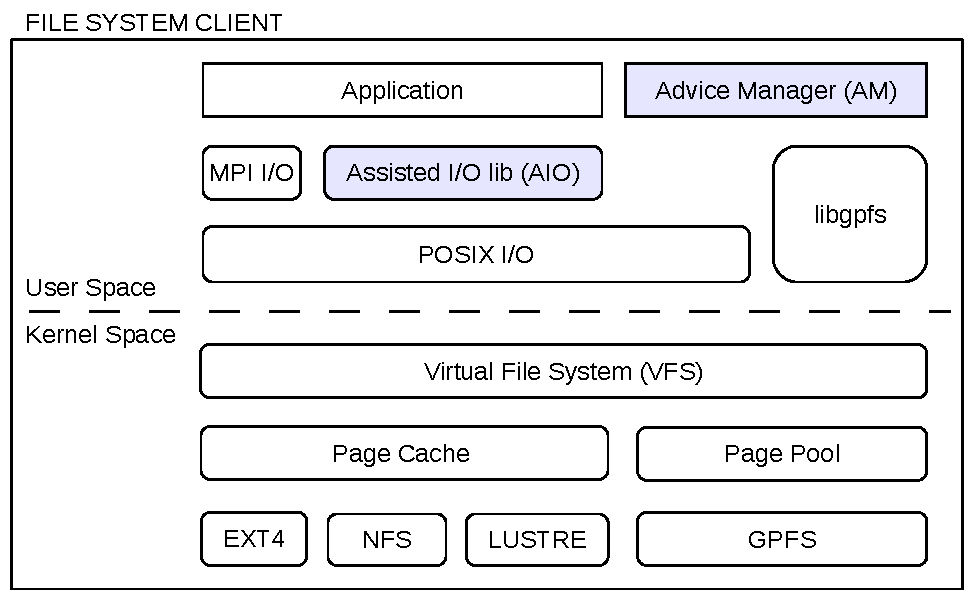
\includegraphics[width=\columnwidth]{advice_paper/figures/softwarestack}
  \caption{MERCURY I/O software stack. \textit{Assisted I/O library} and \textit{Advice Manager} communicate through UNIX domain sockets. %The AM binds its socket to the local file system pathname \texttt{/tmp/channel}, while the IL connects its socket to the same pathname; exactly in the same way they would bind and connect to an IP address if they were located on different nodes in the network. Unix domain sockets are used to pass ancillary data as well as custom messages between the two software entities. 
  Data can reside in a local Linux file system, in Lustre or in GPFS.}
  \label{figure: softwarestack}
\end{figure}

The proposed architecture adds two major contributions. First of all, it allows us to use the Linux advice API as well as the GPFS hints API asynchronously through the \textit{Advice Manager}. This means that we can effectively overlap I/O and computation phases in target applications. Secondly, it enables us to generate POSIX advice and GPFS hints transparently, without the need to modify the application. The information required by the \textit{Advice Manager} is extracted from observations of the application's I/O behaviour~\footnote{How this can be done effectivelly and in a generalized way is itself a research topic and is therefore left as part of future works.} during a set of preliminary runs and then written to a configuration file to be used in following runs.

In the rest of this section we describe the different aspects of our design including the interprocess communication between the two software entities and the prefetching request generation using the \texttt{posix\_fadvise()} system call or the \texttt{gpfs\_fcntl()} function.

\subsection{Interprocess Communication}
\label{subsec: interprocess_comm}
We now describe how interprocess communication is implemented and how messages sent from the \textit{Assisted I/O library} are handled by the \textit{Advice Manager}. Figure~\ref{figure: architecture} depicts the architecture of the two software components introduced by our design. The \textit{Advice Manager} is made up of three smaller modules: a \textit{Request Manager} (RM) that receives requests sent by the \textit{Assisted I/O library}, a \textit{Register Log} (RL) that keeps track of which files are currently handled by the \textit{Advice Manager}, and an \textit{Advisor Thread} (AT) that receives read requests from the \textit{Request Manager} through a queue and issues POSIX advice and GPFS hints.

In order to enable asynchronous prefetching we delegate the task of sending synchronous hints or advice to the \textit{Advice Manager}. When an application issues an open call for a file, the \textit{Assisted I/O library} intercepts it, performs the open and then sends a message to the \textit{Advice Manager}. The message contains a string of the form: \texttt{"\textbf{Register} \textit{pid} \textit{pathname} \textit{fd}"}, plus additional ancillary information explained later. This string tells the \textit{Request Manager} to register the pid of the process opening the file with pathname and file descriptor number, in the register log. As a consequence the \textit{Request Manager} performs two operations, first it asks the \textit{Request Log} to register the new file. From this point on, future read calls for the file will be monitored by the \textit{Advice Manager}. Second, it creates a new \textit{Advisor Thread} that will take care of generating POSIX advice or GPFS hints depending on which file system the file resides in. I/O calls coming from the application are never blocked by the \textit{Assisted I/O library}. The reason is that the \textit{Advice Manager} can become congested by too many requests coming from different processes and we do not want to reflect this on the behaviour of the application.  %The register operation is described by the flow diagram shown in Figure~\ref{figure: register_operation}.

\begin{figure}[!htb]
  \centering
  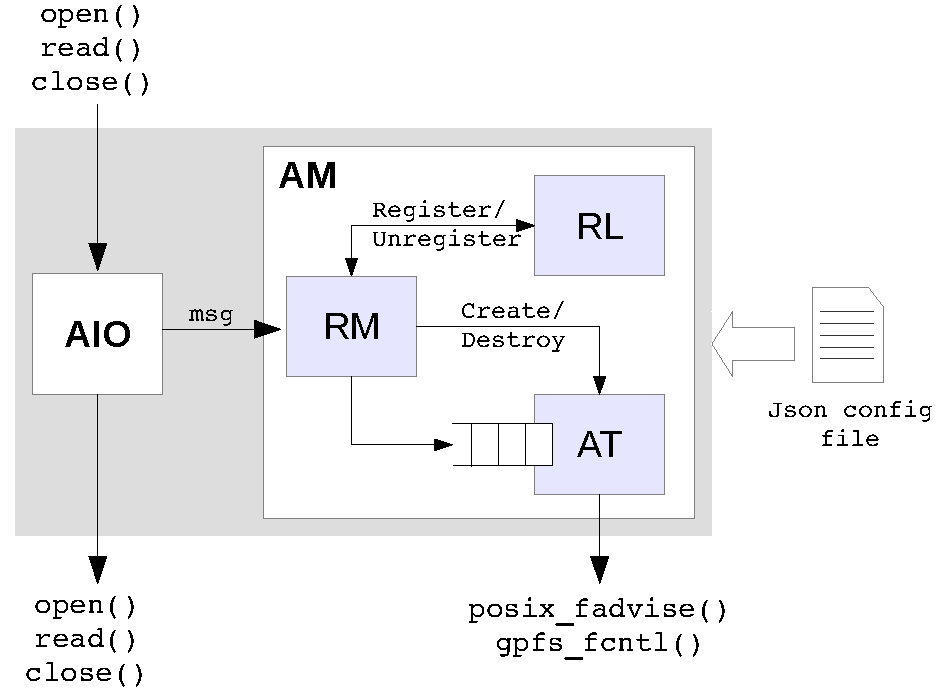
\includegraphics[width=\columnwidth]{advice_paper/figures/architecture}
  \caption{Detailed architecture for the \textit{Advice Manager} (AM) component. This can be further divided into three blocks: \textit{Request Manager} (RM), \textit{Register Log} (RL), and \textit{Advisor Thread} (AT).}
  \label{figure: architecture}
\end{figure}

Both POSIX advice and GPFS hints affect an open file, identified by its file descriptor number. For the \textit{Advice Manager} to send advice or hints on behalf of the application, it needs to share the open file with the application. When sending messages from the \textit{Assisted I/O library} to the \textit{Advice Manager} we use \texttt{sendmsg()}. Besides normal data, this system call allows the transfer of ancillary (or control) information. One use of such information is to send a remote process a 'file descriptor'~\cite{StevensR13} via a UNIX domain socket~\cite{UnixSock}. These numbers are just an index into the kernel's list of a process's open files. When sending a file descriptor using \texttt{sendmsg()}, the kernel copies a new reference to the open file descriptor, and adds it to the receiving process's open files list. The \textit{Advice Manager} receives a new file descriptor number, (which will likely be different to the number sent), which points to a file descriptor shared with the application. This allows us to send hints or advice for the shared file.

\subsection{File Data Prefetching}
\label{subsec: data_prefetching}
POSIX advice and GPFS hints are issued using the \textit{Advisor Thread} created by the \textit{Request Manager} during the register operation (Figure~\ref{figure: architecture}). When an application performs a read operation for an open file, the \textit{Assisted I/O library} sends to the \textit{Advice Manager} a message containing a string of the form: \texttt{"\textbf{Read} \textit{pid} \textit{fd} \textit{off} \textit{len}"}. This string includes the pid of the process, the application's file descriptor number for the file, the offset within the file and the length of the request. The pid and the file descriptor number are used by the \textit{Request Manager} module only to identify the corresponding \textit{Advisor Thread}. When the correct thread has been identified the \textit{Request Manager} pushes the offset and the length of the read request into a queue. This queue is accessed by the \textit{Advisor Thread} that uses the read information to trigger prefetch requests using the local file descriptor and keeps track of all the prefetched data using a block cache data structure. %Figure~\ref{figure: read_operation} shows the flow diagram for the read operation. 

The \textit{Advisor Thread} uses \texttt{posix\_fadvise()} and \texttt{gpfs\_fcntl()} to generate prefetch requests for the underlying file systems (Figure~\ref{figure: architecture}). For files residing in local file systems and Lustre, the \texttt{POSIX\_FADV\_WILLNEED} advice from Table~\ref{table: advice_table} is used to bring the data into the kernel page cache. For files residing in GPFS the \texttt{accRangeArray} in the \texttt{gpfsMultipleAccessRange\_t} data structure in Listing~\ref{mar} is used to define which blocks of the file should be brought into the GPFS internal cache (page pool). 
The size of the file regions to prefetch is defined in a Json\footnote{Open standard format that uses human-readable text to transmit data objects consisting of attribute-value pairs (http://www.rfc-editor.org/rfc/rfc7159.txt).} configuration file, loaded at startup by both the \textit{Advice Manager} and the \textit{Assisted I/O library}. This is the only point of configuration for the user and it contains, besides other information, a list of files and directories that the \textit{Assisted I/O library} should monitor. An example configuration file is shown below. 
\lstset{
        captionpos=b,
        language=python,
        keywordstyle=\color{blue}\footnotesize\ttfamily,
        breaklines=true,
        basicstyle=\footnotesize\ttfamily,
        caption={Example of Json configuration file.},
        label=config
}
\begin{lstlisting}[frame=single]
{
    "File": [
    {
        "Path": "/path/to/target/file",
        "BlockSize": 4194304,
        "CacheSize": 8,
	"ReadAheadSize": 4,
        "WillNeed": [
        {
            "Offset": 0,
            "Length": 0
        }]
    }],
    "Directory": [
    {
        "Path": "/path/to/target/dir",
        "Random": [
        {
            "Offset": 0,
            "Length": 0
        }]
    }]
}
\end{lstlisting}
As it can be seen in Listing~\ref{config} the structure of the configuration file is very simple. It allows users to define which files POSIX advice or GPFS hints should be applied to by setting the `Path' field to the full file path and the regions of the file that are likely to be accessed in terms of offset and length. In the case of POSIX advice users can also define directories to which a global advice should be applied (e.g. randomly accessed files in the directory). Additionally, when indicating a `WillNeed' advice users can directly control the caching behaviour of the \textit{Advisor Thread} block cache. In particular, they can define the granularity of the prefetch request (`BlockSize'), how many blocks can be fitted into the \textit{Advisor Thread} cache (`CacheSize') and how many blocks of data should be read ahead starting from the current accessed block (`ReadAheadSize'). % and in general the configuration file can contain precise information describing the I/O behavior of the application. %In conclusion, by providing configuration files that can match file names, file sizes or even file regions advice and hints should be applied to, administrators or automatized tools can dynamically change the I/O prefetch patterns in order to best fit their needs.
%TODO: is there a citation available for advice on directories?
Clearly the example in Listing~\ref{config} is not exhaustive. More complex configuration files can be generated by administrators (or automatic tools) to dynamically change the I/O patterns of applications in order to best adapt them to the underlying storage system. %For example there may be a preferred block size for files stored in a particular file system

%\begin{algorithm}[h]
% \KwData{sequence of prefetch ranges: \textit{config}, current request offset and length: \{\textit{off}, \textit{len}\}}
% \KwResult{a prefetch request vector: \textit{prefetch}} 
% \While{true}{
%  $off \leftarrow request\ offset$\;
%  $len \leftarrow request\ length$\;
%  \eIf{understand}{
%   go to next section\;
%   current section becomes this one\;
%   }{
%   go back to the beginning of current section\;
%  }
% }
% \caption{GPFS Prefetching Algorithm in the Advisor Thread.}
%\end{algorithm}
The replacement policy for the block cache in the \textit{Advisor Thread} uses an LRU algorithm. In order to prefetch data, the open file is divided into blocks of size `BlockSize' and entire blocks are loaded/released into/from memory as the application progresses. In the case of GPFS the \texttt{accRangeArray} hint is used to prefetch up to `ReadAheadSize' blocks ahead starting from the block touched by the current request. When the number of blocks in the cache has reached `CacheSize', if more blocks are requested, older blocks will be released using the \texttt{relRangeArray} hint to make space for the new ones. In the case of POSIX advice, the behaviour is the same but blocks are loaded into memory using the \texttt{POSIX\_FADV\_WILLNEED} advice and released using the \texttt{POSIX\_FADV\_DONTNEED} advice. The hints interface is automatically selected by the \textit{Advice Manager} at runtime depending on the file system hosting the target file. 
%The only exception is when the prefetch region is bigger than 16MB. In this case the file range is broken down into smaller ranges of 4MB and each of them is prefetched separately. This prevents a very large `WillNeed' section from flooding the page cache at one time (e.g. if the all data of a big file has to be prefetched sequentially). 
%By keeping track of what data has been already prefetched the \textit{Advisor Thread} can also avoid new coming requests triggering the prefetch of the same data. 
%During the time between an open and a close operation the \textit{Advisor Thread} also avoids multiple reads triggering advice and (or) hints for the same block in the file by keeping track of all the currently prefetched blocks. If a new read requests a block already prefetched the read will be ignored. When a block is no longer needed the \textit{Advisor Thread} releases it using either \texttt{POSIX\_FADV\_DONTNEED} or the \texttt{relRangeArray} in Listing~\ref{mar}. 

The \textit{Advisor Thread} block cache also provides a very basic level of coordination among processes accessing the same file. In fact, different \textit{Advisor Thread} instances hinting the same file on behalf of different processes share the same block cache. Blocks requested by one process will appear in the block cache and future accesses to those blocks by other processes will not trigger new prefetching requests.

%At the moment the prefetching algorithm used by the \textit{Advisor Thread} is very simple. It assumes that file ranges in a \texttt{WillNeed} section of the configuration file are accessed in sequential order by the application. In the case of GPFS the \texttt{accRangeArray} is used to prefetch up to \texttt{GPFS\_MAX\_RANGE\_COUNT} blocks ahead of the current request. When the application requests data that is \texttt{GPFS\_MAX\_RANGE\_COUNT/2} blocks away from the last prefetched block, another eight blocks of data are prefetched. On the other hand requested blocks that are no longer needed are released in groups of \texttt{GPFS\_MAX\_RANGE\_COUNT/2} using the \texttt{relRangeArray}. In the case of POSIX advice the algorithm is the same but instead of blocks it considers file ranges contained in the \texttt{WillNeed} section as a single prefetch unit for \texttt{POSIX\_FADV\_WILLNEED}. By keeping track of what data in the file has been already prefetched the \textit{Advisor Thread} can prevent new requests from triggering a prefetch of the same data. %During the time between an open and a close operation the \textit{Advisor Thread} also avoids multiple reads triggering advice and (or) hints for the same block in the file by keeping track of all the currently prefetched blocks. If a new read requests a block already prefetched the read will be ignored. When a block is no longer needed the \textit{Advisor Thread} releases it using either \texttt{POSIX\_FADV\_DONTNEED} or the \texttt{relRangeArray} in Listing~\ref{mar}. 
%\todo[inline]{this should be replaced or extended by a formal description of the algorithm ...}

In general the configuration file can be used to describe any of the advice listed in Table~\ref{table: advice_table} and the hints listed in Table~\ref{table: hints_table}. To define a new scenario, we may consider a file region accessed sequentially for which the \texttt{POSIX\_FADV\_SEQUENTIAL} advice type could be used, and another region accessed randomly for which the \texttt{POSIX\_FADV\_RANDOM} advice type could be used. In this case, the configuration file would contain a list of file regions, specifying which type of advice messages are suitable. The right advice will be selected according to which part of the file is being accessed currently. This feature allows us to overcome another limitation of the Linux advice implementation that has been mentioned in Section~\ref{subsec: posix_advice_api}, namely, the first three advice types apply to the whole file since the implementation in the kernel completely disregards the byte ranges specified by the user.
 
Finally, when the application closes the file the \textit{Assisted I/O library} sends to the \textit{Advice Manager} a message containing a string of the form: \texttt{"\textbf{Unregister} \textit{pid} \textit{fd}"}. This string includes the pid of the process and the file descriptor number of the file to be closed. In response to this request the \textit{Request Manager} tells the \textit{Register Log} to unregister the file and destroys the \textit{Advisor Thread}, it also closes its shared copy of the file.

\subsection{POSIX Advice integration with Lustre}
\label{subsec: posix_advice_lustre}
Lustre is a high performance parallel file system for Linux clusters. It works in kernel space and takes advantage of the available page cache infrastructure. Additionally, it extends POSIX read and write operations with distributed locks to provide data consistency across the whole cluster. Even though Lustre makes use of the Linux kernel page cache, the previously described POSIX advice syscall has no effect on Lustre. The reason can be understood by looking at Figure~\ref{figure: kernel}. This reports the simplified call graph for the Lustre read operation in the file system client. To simplify the explanation, the figure is divided into four quadrants. Along the x-axis we have the native kernel functions (e.g. \texttt{generic\_file\_aio\_read}), separated by the Lustre specific functions (e.g. \texttt{lustre\_generic\_file\_read}). Along the y-axis we have page operations (e.g. \texttt{find\_get\_page}) separated by the file operations (e.g. \texttt{generic\_file\_aio\_read}). 

We can notice that Lustre extends the kernel code with additional file and page operations through the Lustre Lite component. These are the functions used by the kernel to fill the file operations table and the address space operations table. The \texttt{posix\_fadvise()} system call in the kernel translates into \texttt{fadvise64()}. In the case of \texttt{POSIX\_FADV\_WILLNEED} this function directly invokes \texttt{force\_page\_cache\_readahead()} which has no effect on \texttt{ll\_readpage()}. Other advice such as \texttt{POSIX\_FADV\_\{NORMAL,SEQUENTIAL,RANDOM\}} are disabled in Lustre by setting the kernel read-ahead window size to zero. This is done so that lustre will not speculatively try to gain a highly-contended lock to fulfil an optimistic read-ahead request.

\begin{figure}[!htb]
  \centering
  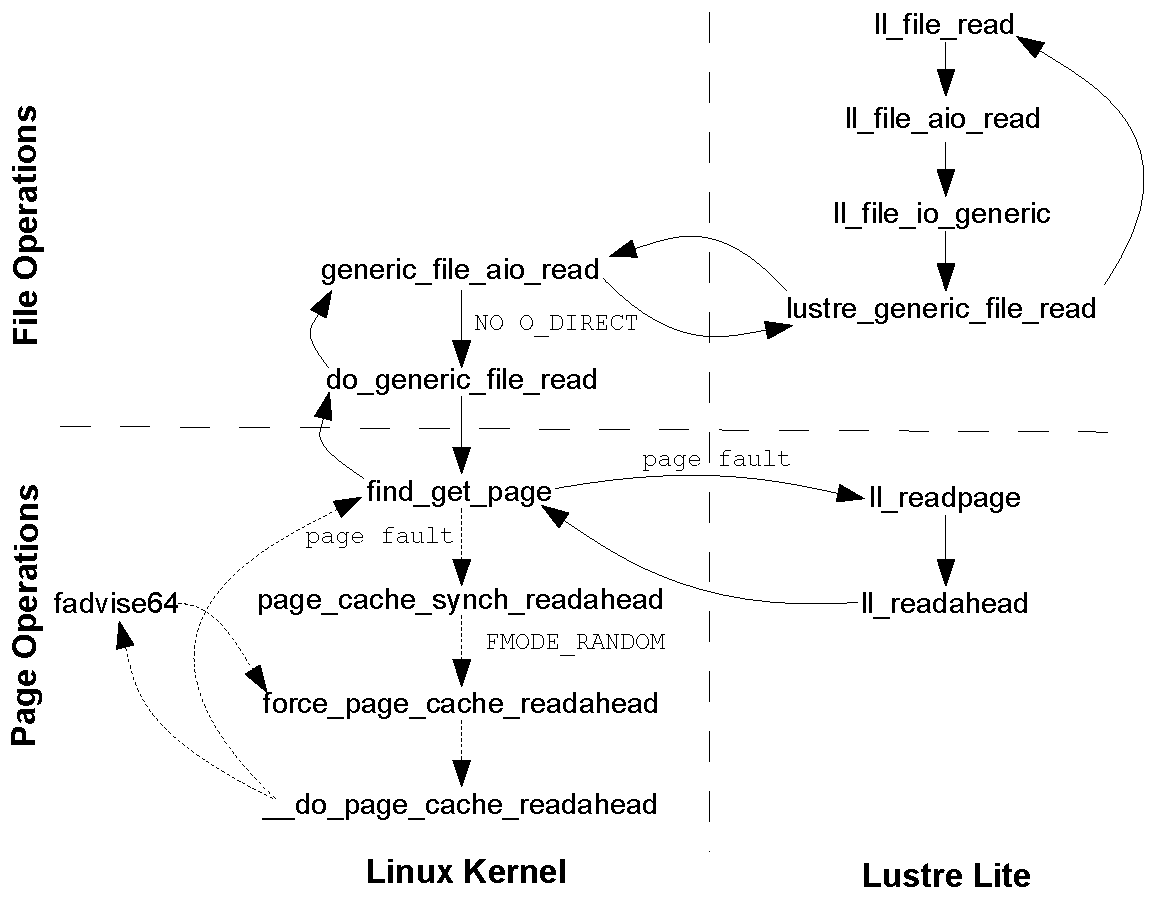
\includegraphics[width=\columnwidth]{advice_paper/figures/kernel}
  \caption{Simplified function call graph for the read operation in Lustre. For page operations in the Linux kernel the picture also shows the call graph typically followed by local reads as well as the call graph for the \texttt{POSIX\_FADV\_WILLNEED} advice in the \texttt{posix\_fadvise()} implementation (dashed line).}
  \label{figure: kernel}
\end{figure}

% This paragraph could be explained more clearly - you are effectivly filling the file system cache, on the assumption that it is the page-cache, instead of filling the page cache. This allows file systems that don't interface directly with the page cache to work.
In order to enable \texttt{POSIX\_FADV\_WILLNEED} in Lustre we modified the call graph of \texttt{fadvise64()} presented in Figure~\ref{figure: kernel} to invoke the \texttt{aio\_read()} operation in the file operations table for the open file and block until all the data has been read into the page cache. In this way we can force the kernel to invoke the corresponding file read operation in Lustre, acquiring locks as appropriate. Of course this mechanism still works with local file systems which eventually will end up calling \texttt{force\_page\_cache\_readahead()} as in the original version.

To prevent the new generated read from altering the read-ahead state of normal read operations, in \texttt{fadvise64()} we create a new \texttt{struct file} using the \texttt{dentry\_open()} routine and set the access mode flag (\texttt{f\_mode}) of the new file to \texttt{FMODE\_RANDOM} (which is exactly what the \texttt{POSIX\_FADV\_RANDOM} advice message does to disable read-ahead for random accessed files). This mechanism works perfectly with local file systems but has no effect on Lustre's read-ahead algorithm which is independent from the Linux kernel read-ahead. Therefore, \texttt{POSIX\_FADV\_WILLNEED} in the case of Lustre prefetches a bit more data than requested. This is acceptable for now but a future implementation will also modify the Lustre code to make sure the behaviour is the same in both cases.

Finally, our kernel patch does not require any user buffer to be provided with the new read operation. To avoid data being copied to user space we pass a null pointer to the \texttt{aio\_read()} routine. Additionally we defined a new \texttt{ki\_flag} for the kernel I/O control block (\texttt{kiocb}), that we called \texttt{KIF\_FORCE\_READ\_AHEAD}. This new flag is checked in the \texttt{generic\_file\_aio\_read()} routine and if set the \texttt{do\_generic\_file\_read()} routine is invoked with a pointer to the \texttt{file\_read\_actor\_dummy()} routine. \texttt{file\_read\_actor()} is normally the routine responsible for copying the data from the page cache to the user space buffer. Since in our case there is no user space buffer, the dummy routine just returns success.

%!TEX root = ../main.tex
\section{Evaluation}
\label{sec: results}
To evaluate the proposed MPI-IO hints we use three popular I/O benchmarks frequently adopted to profile collective I/O performance in other research works: coll\_perf\footnote{Collective I/O benchmark distributed with the MPICH package.}, Flash-IO and IOR.
Minor changes to the source code of the three benchmarks have been made to adapt them to our needs. For example, coll\_perf and Flash-IO do not support writing to multiple files and the emulation of computing delays. Thus, we modified them to reproduce the workflow shown in Figure~\ref{figure: workflow3}. The number of written files and a compute delay are now parameters that can be passed from the command line. In all our tests we used 512 MPI processes distributed over 64 nodes (8 procs/node), fixed the file stripe size to 4~MB and the stripe count to 4. Moreover, for simplicity, we also fixed the size of the cache synchronisation buffer (i.e. \codeword{ind\_wr\_buffer\_size}) to 512~KB, which corresponds to the standard independent I/O buffer size. On the other hand, we varied the collective I/O parameters, i.e., the number of aggregators (from 8 to 64) and the collective buffer size (from 4~MB to 64~MB). For every combination of these parameters (<aggregators>\_<coll\_bufsize>) each benchmark writes four files of the same size (32~GB) with a compute delay of 30 seconds, which is in most cases enough to hide the synchronisation time. We compute the bandwidth as the average bandwidth over the four collective write operations (Equation~\ref{formula: abw}). The different  contributions within the collective I/O write path shown in Figure~\ref{figure: coll_io_impl} are extracted from the ROMIO layer using MPE profiling~\cite{mpe}.
Whenever the compute delay is not enough to hide synchronisation (e.g. when a small number of aggregators is used), the remaining synchronisation time is added to the total write time, thus reducing the bandwidth.

\subsection{Testbed}
\label{subsec: testbed}
Our testbed is a research cluster designed and developed in the context of the DEEP/-ER~\cite{deep}\cite{deep-er} projects (Dynamic Exascale Entry Platform/-Extended Reach). The DEEP/-ER cluster has 2048 cores distributed over 128 computing nodes (dual socket Sandy Bridge architecture). The storage system is composed of 6 Dell PowerEdge R520 servers equipped with 2 Intel Xeon Quad-core CPUs and 32~GB of memory and run the BeeGFS file system from Fraunhofer ITWM~\cite{fhgfs} (formerly known as FhGFS). The servers are connected to a SGI JBOD with 45 2TB SAS drives through a SAS switch using two 4x ports at 6~GB/s, for a total of four 8+2 RAID6 storage targets and 2 RAID1 targets for metadata and management data (1 drive is left as spare). One of the six I/O servers is dedicated as metadata server, one as management server and the remaining four as data I/O servers.
Additionally, every compute node is equipped with 32~GB of RAM memory and a 80~GB SATA SSD containing the operating system plus an additional 30~GB ext4 partition (mounted under `/scratch') for general purpose storage. This partition, in our case, is used to locally cache collective writes. Finally, all the computing nodes are connected through an Infiniband QDR network and use ParaStation MPI~\cite{parastation} (PSMPI) version 5.1.0-1 as message passing library.

\subsection{Coll\_perf}
\label{subsec: coll_perf}
In our coll\_perf configuration every process writes one 64~MB block being part of a tridimensional distributed array to a shared file, thus generating a strided pattern. For every experiment, in which we vary the number of aggregators and the collective buffer size, we measure the coll\_perf perceived write bandwidth in three different cases: \textit{1}) when writing directly to the global file system (BW Cache Disabled), \textit{2}) when writing to the cache (BW Cache Enabled) and afterwards flushing its content to the global file system asynchronously, and \textit{3}) when writing to the cache without flushing its content to the global file system (TBW Cache Enable). The last case provides the theoretical bandwidth achievable when the cache synchronisation cost is completely hidden. Additionally, our coll\_perf experiments do not include the last write phase contribution (Figure~\ref{figure: workflow3}). In fact, for the last write the cache synchronisation cost cannot be hidden since there is no following compute phase. We will show the effect that the last write has on the average bandwidth of the IOR benchmark at the end of this evaluation.

Figure~\ref{figure: collperf-bw} shows the write bandwidth for the three cases previously discussed.
\begin{figure}[b!]
  \centering
  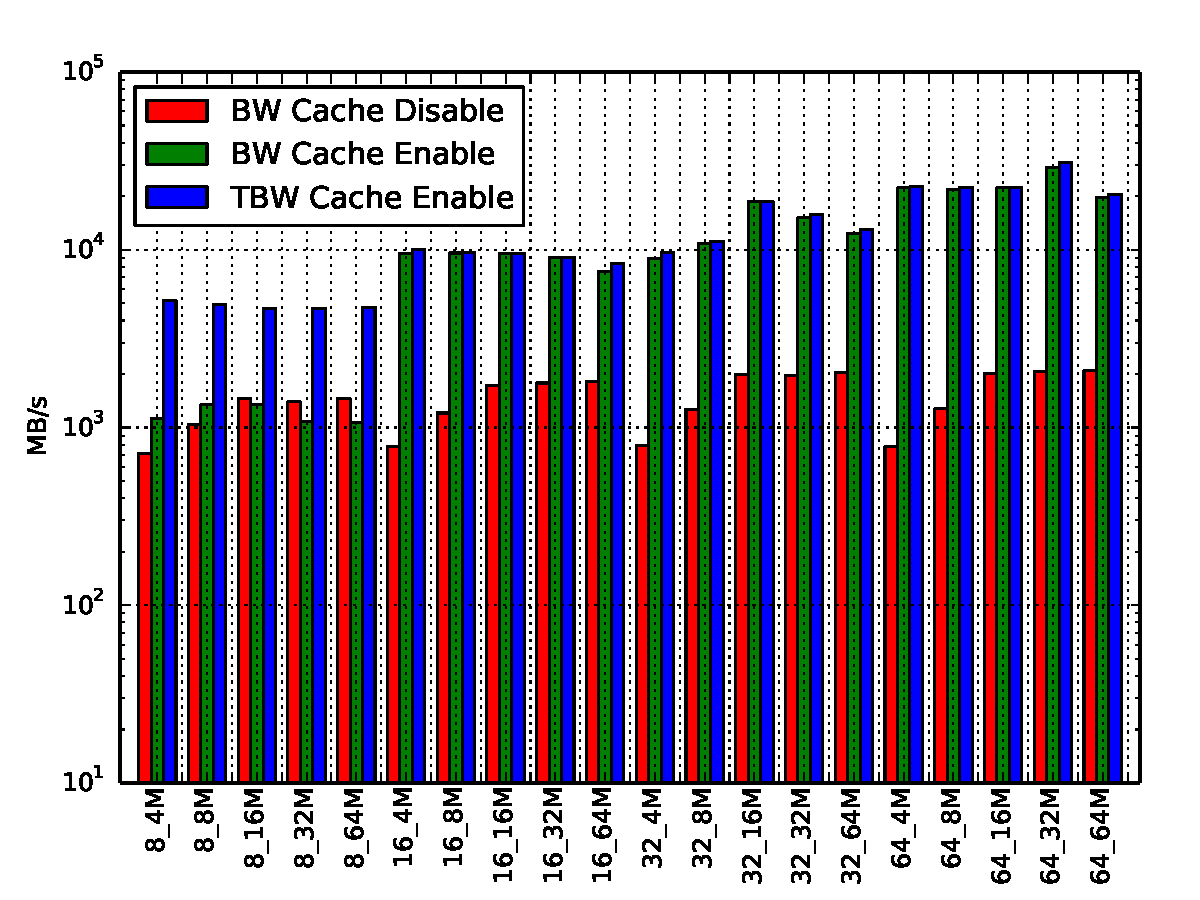
\includegraphics[width=0.95\columnwidth]{figures/coll_perf_32GB_30sec_bw}
  \caption{coll\_perf perceived bandwidth for all combinations of <aggregators>\_<coll\_bufsize>.} % The figure also shows the theoretical bandwidth (TBW) when the cache is not flushed.}
  \label{figure: collperf-bw}
\end{figure}
First of all, we can observe that for most of the experiments the aggregate bandwidth when using the cache is higher than the bandwidth measured when using only the global file system. In particular, we can reach a peak performance of about 20~GB/s, compared to the 2~GB/s of the standard case (BW Cache Disabled), which gives a ten fold improvement. Second, when the number of aggregators is equal to 8, we notice a reduced performance, as the synchronisation cost cannot be completely hidden.

\begin{figure}[b!]
  \centering
  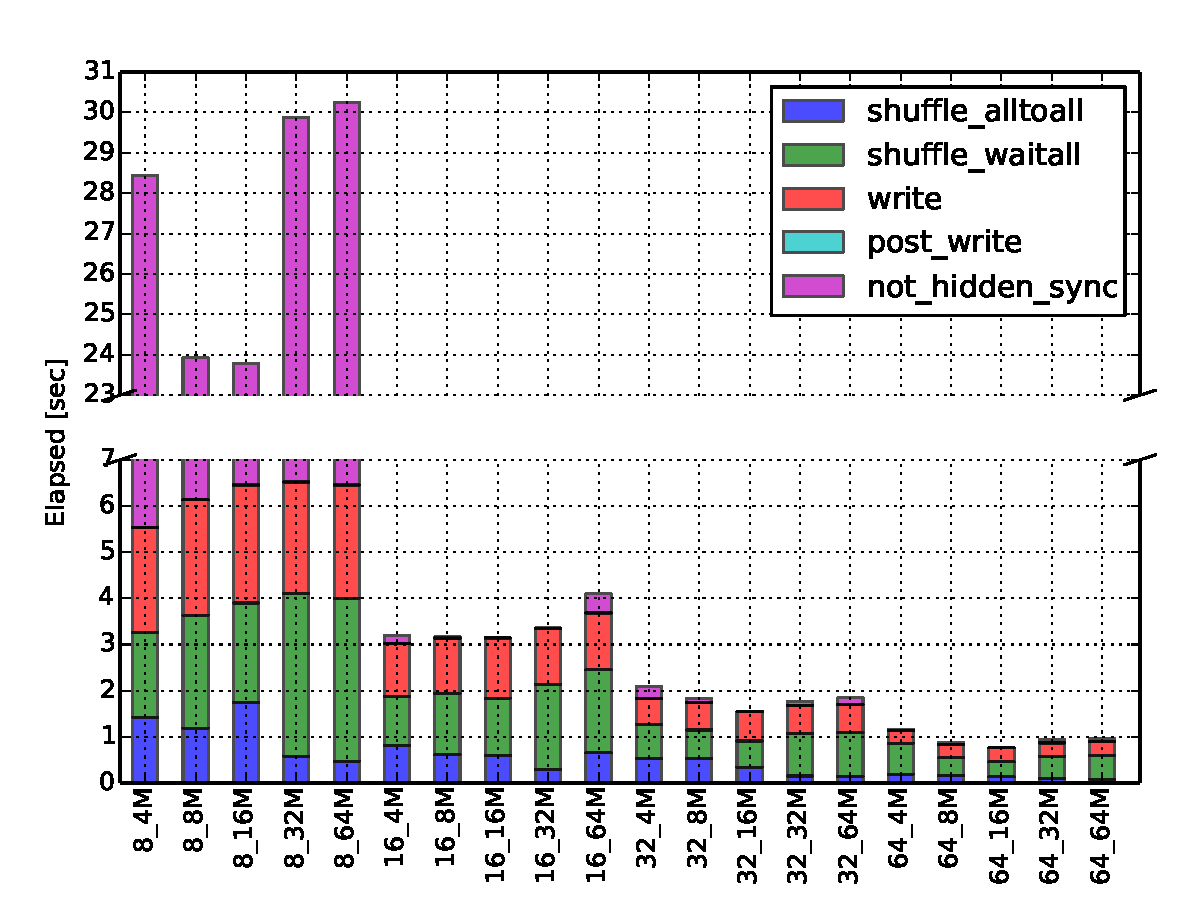
\includegraphics[width=0.95\columnwidth]{figures/coll_perf_32GB_30sec_elapsed_enable}
  \caption{coll\_perf collective I/O contribution breakdown when cache is enabled.} % When the number of aggregators is 8 we clearly see the effect of synchronisation.}
  \label{figure: collperf-elaps-enable}
\end{figure}
The effect of the non-hidden cache synchronisation (not\_hidden\_sync) is shown in Figure~\ref{figure: collperf-elaps-enable}. This figure presents the collective I/O performance breakdown for all the components shown in Figure~\ref{figure: coll_io_impl}. As we can see, although the theoretical bandwidth (TBW Cache Enable) peaks at 4~GB/s (Figure~\ref{figure: collperf-bw}), the measured bandwidth (BW Cache Enable) can be even worse than the standard case (BW Cache Disable). This happens because the cache data cannot be flushed to the global file system quickly enough. In all the other experiments, the perceived and theoretical bandwidth are well aligned.

\begin{figure}[htb]
  \centering
  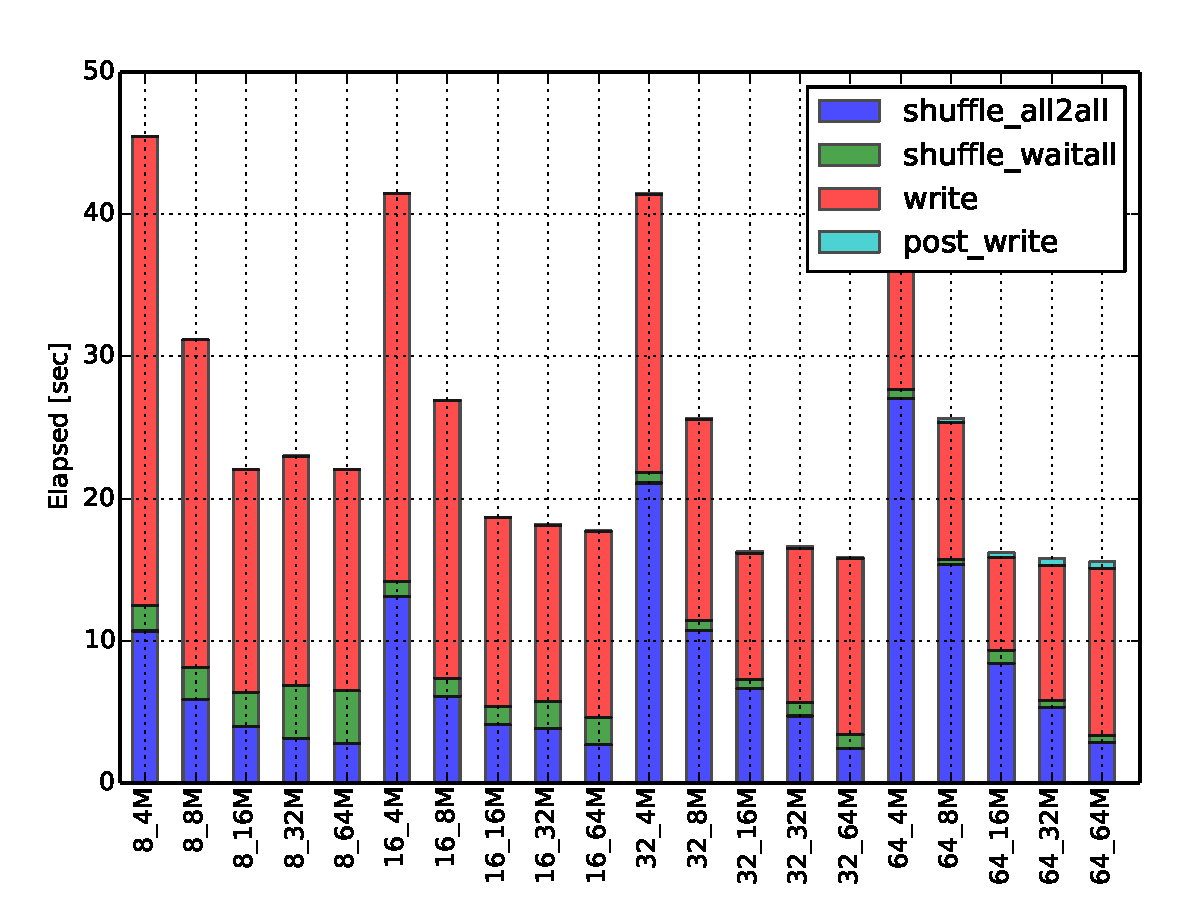
\includegraphics[width=0.95\columnwidth]{figures/coll_perf_32GB_30sec_elapsed_disable}
  \caption{coll\_perf collective I/O contribution breakdown when cache is disabled.}
  \label{figure: collperf-elaps-disable}
\end{figure}

As already said in the previous sections, our SSDs based approach can also help to reduce the global synchronisation cost in the extended two phase I/O algorithm at the base of collective I/O.
In fact, by comparing Figures~\ref{figure: collperf-elaps-enable} and~\ref{figure: collperf-elaps-disable}, we see that the global synchronisation costs in collective I/O, represented by \codeword{MPI\_Alltoall()} (shuffle\_all2all) and \codeword{MPI\_Allreduce()} (post\_write) are consistently reduced when using the cache.

Finally, we observe that most of the times, when using the cache, larger collective buffers do not produce large performance improvements. This means that we can achieve good performance with small buffers and thus reduce the memory pressure of collective write operations on compute nodes.

\subsection{Flash-IO}
\label{subsec: flash}
Flash-IO is the I/O kernel of the Flash application. Flash is a block-structured adaptive mesh hydrodynamics code. The computational domain is divided into blocks which are distributed across the processors. Typically a block contains 16 zones in each coordinate direction (x,y,z) and a perimeter of guard cells (presently 4 zones deep) to hold information from the neighbors. The application writes three files using the parallel HDF5 library: a checkpoint file, a plot file without corner data and a plot file with corner data. The checkpoint file is the biggest of the three and consumes the majority of the I/O time. In our configuration the checkpoint file contains 80 blocks/process and each of the 16 zones/block contains 24 variables encoded with 8bytes (768~KB/proc/block). Therefore, the total size is slightly bigger than 30~GB (including metadata).

\begin{figure}[t!]
  \centering
  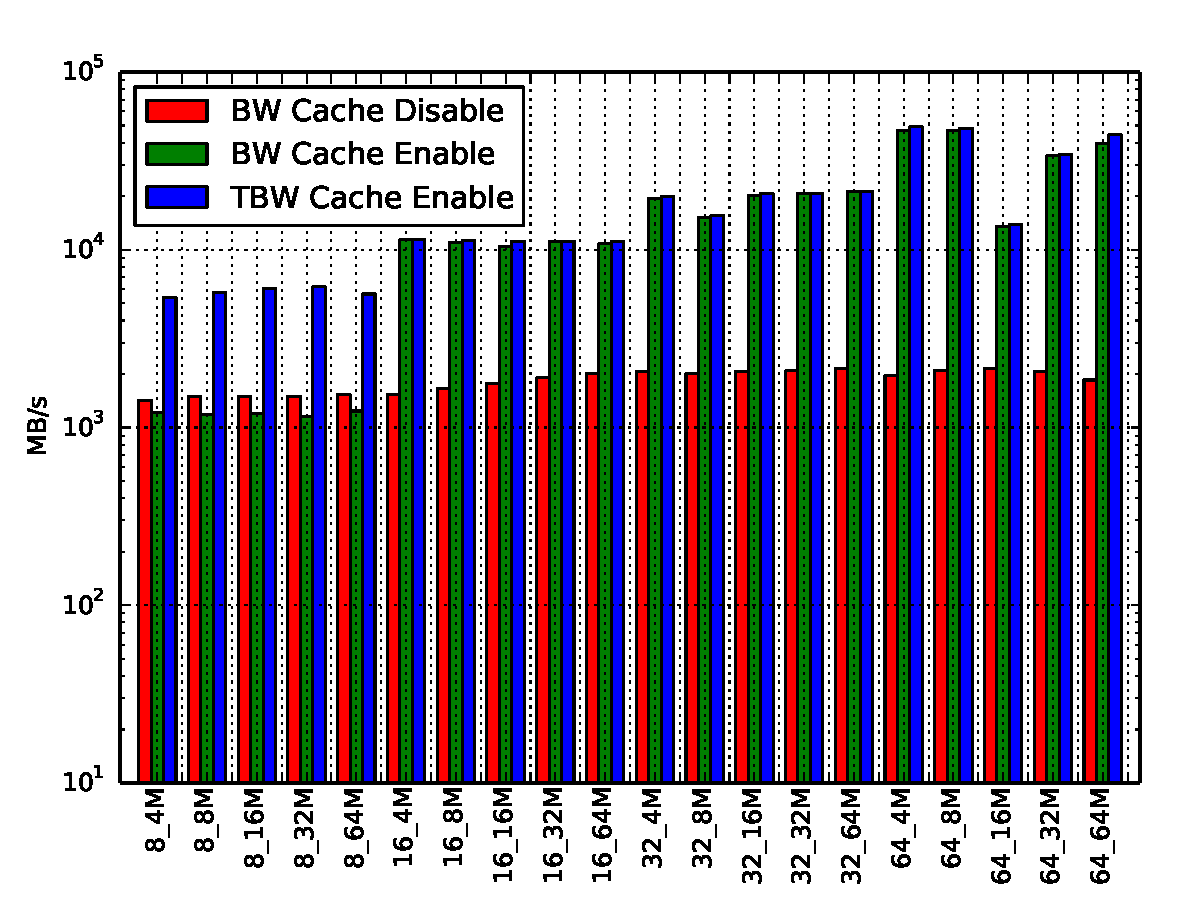
\includegraphics[width=0.95\columnwidth]{figures/flash_32GB_30sec_bw}
  \caption{Flash-IO perceived bandwidth for all combinations of <aggregators>\_<coll\_bufsize>.} %The figure also shows the theoretical bandwidth (TBW) when the cache is not flushed.}
  \label{figure: flash-bw}
\end{figure}

Figure~\ref{figure: flash-bw} shows the write bandwidth perceived by Flash-IO for all the experiments performed in the different cases under study. Similarly to coll\_perf, when the cache is enabled we can hide the cache synchronisation cost for most of the experiments. Once again, like in the previous case, when the number of aggregators is equal to 8 we have a mismatch between the perceived and the theoretical bandwidth. For Flash-IO the peak bandwidth is about 40~GB/s when using 64 aggregators and 4~MB collective buffer size, against the 2~GB/s measured when writing directly to the parallel file system.
\begin{figure}[htb]
  \centering
  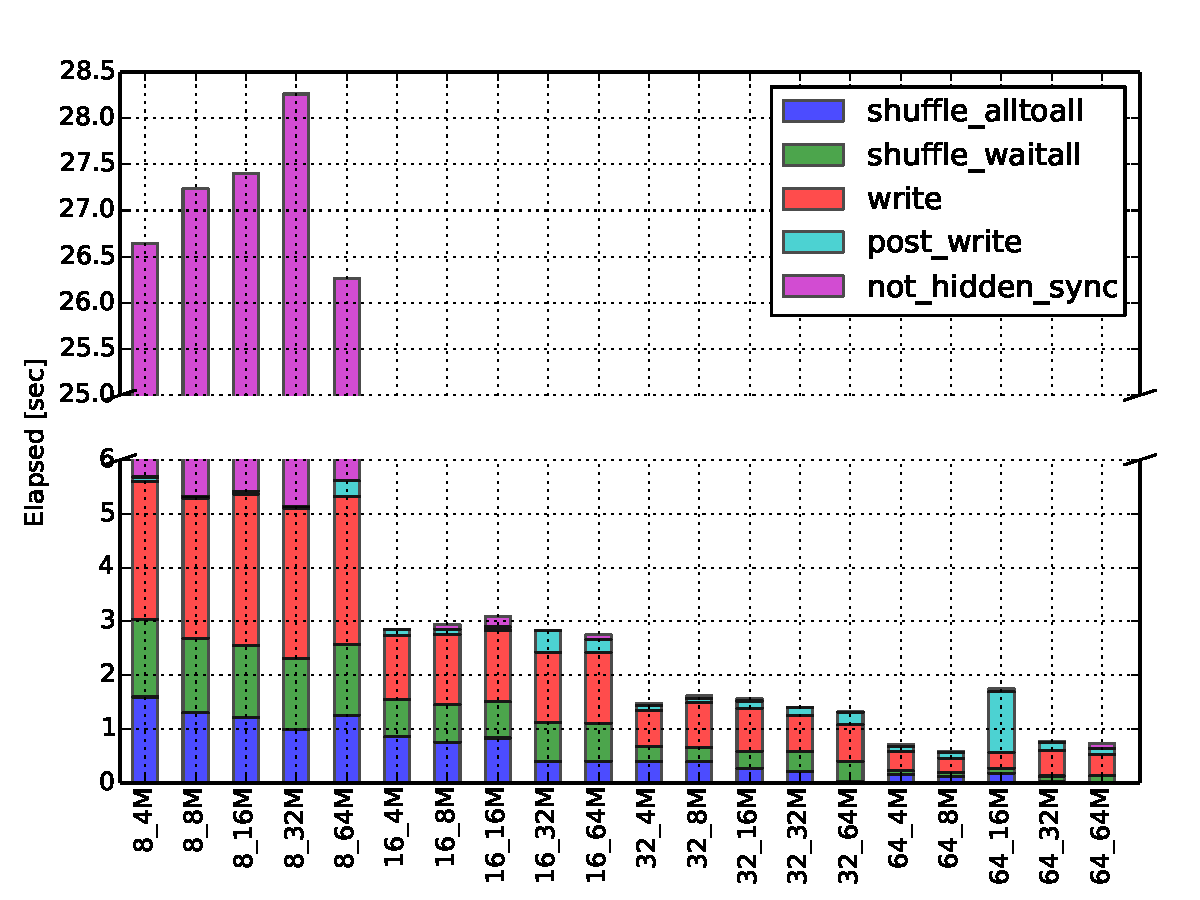
\includegraphics[width=0.95\columnwidth]{figures/flash_32GB_30sec_elapsed_enable}
  \caption{Flash-IO collective I/O contribution breakdown when cache is enabled.}
  \label{figure: flash-elaps-enable}
\end{figure}

Figure~\ref{figure: flash-elaps-enable} shows the effect of cache usage on the different collective I/O performance contributions. We can clearly see that when the number of aggregators is equal to 8 the cache synchronisation cannot be completely hidden, causing the bandwidth mismatch previously observed in Figure~\ref{figure: flash-bw}. Furthermore, like in the coll\_perf case the global synchronisation contributions can be reduced when using the cache, and so can the memory pressure on the compute nodes.
\begin{figure}[htb]
  \centering
  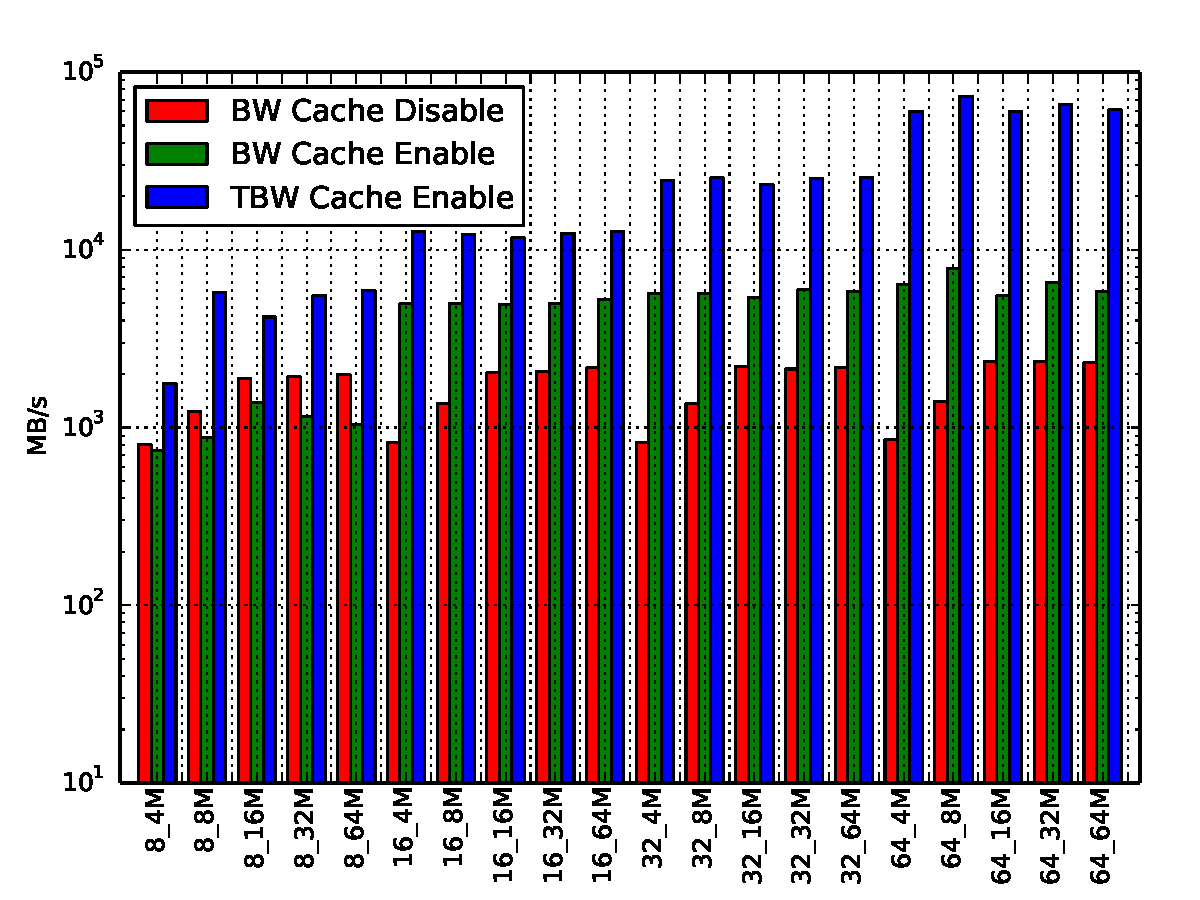
\includegraphics[width=0.95\columnwidth]{figures/ior_32GB_30sec_bw}
  \caption{IOR perceived bandwidth for all combinations of <aggregators>\_<coll\_bufsize>.} %The figure also shows the theoretical bandwidth (TBW) when the cache is not flushed.}
  \label{figure: ior-bw}
\end{figure}
Nevertheless, for the 64 aggregators and 16~MB collective buffer size configuration the global synchronisation overhead associated to \codeword{MPI\_Allreduce()} (post\_write) has a larger value. The outlier causes a strong reduction in the write bandwidth, although we can still achieve more than 10~GB/s. This indicates that the effect of global synchronisation when using the cache can be even more severe, due to the much higher bandwidth achievable compared to the standard global file system approach.

\subsection{IOR}
\label{subsec: ior}
We tested IOR when writing collectively to a shared file. Each of the 512 MPI processes writes one 8~MB block of data for each of the 8 segments, that is, a 32~GB file during every test.
%\todo[inline]{remove standard deviation explanation and focus on the last part where the real reason for reduced performance is exposed. explain that add one additional read and one additional write is making things worse when using a small number of SSD/aggregators. improve figures adding bars for synchronization cost separately. add a reference to the statement that large systems might not be able to write concurrently to all the available I/O targets.}
%\todo[inline]{reading data back from the cache: illustrate problems related to additional metadata information required (example ADIOS does this using a custom binary format). describe this in related or future work.}
As for the previous two benchmarks, Figure~\ref{figure: ior-bw} shows the write bandwidth perceived by IOR. Nevertheless, unlike the previous benchmarks, in IOR we also take into account the non-hidden synchronisation cost coming from the last write phase. In this case, the peak bandwidth when using the cache can reach about 6~GB/s versus the 2~GB/s of the standard collective write to the global file system. We can also see that the theoretical bandwidth is aligned with the figures presented for coll\_perf and Flash-IO. In fact, although we can hide cache synchronisation costs for the three intermediate write phases in IOR, the fourth write phase will limit the peak performance.

Figures~\ref{figure: ior-elaps-enable} shows the collective I/O cost breakdown for all the time contributions. 
\begin{figure}[htb]
  \centering
  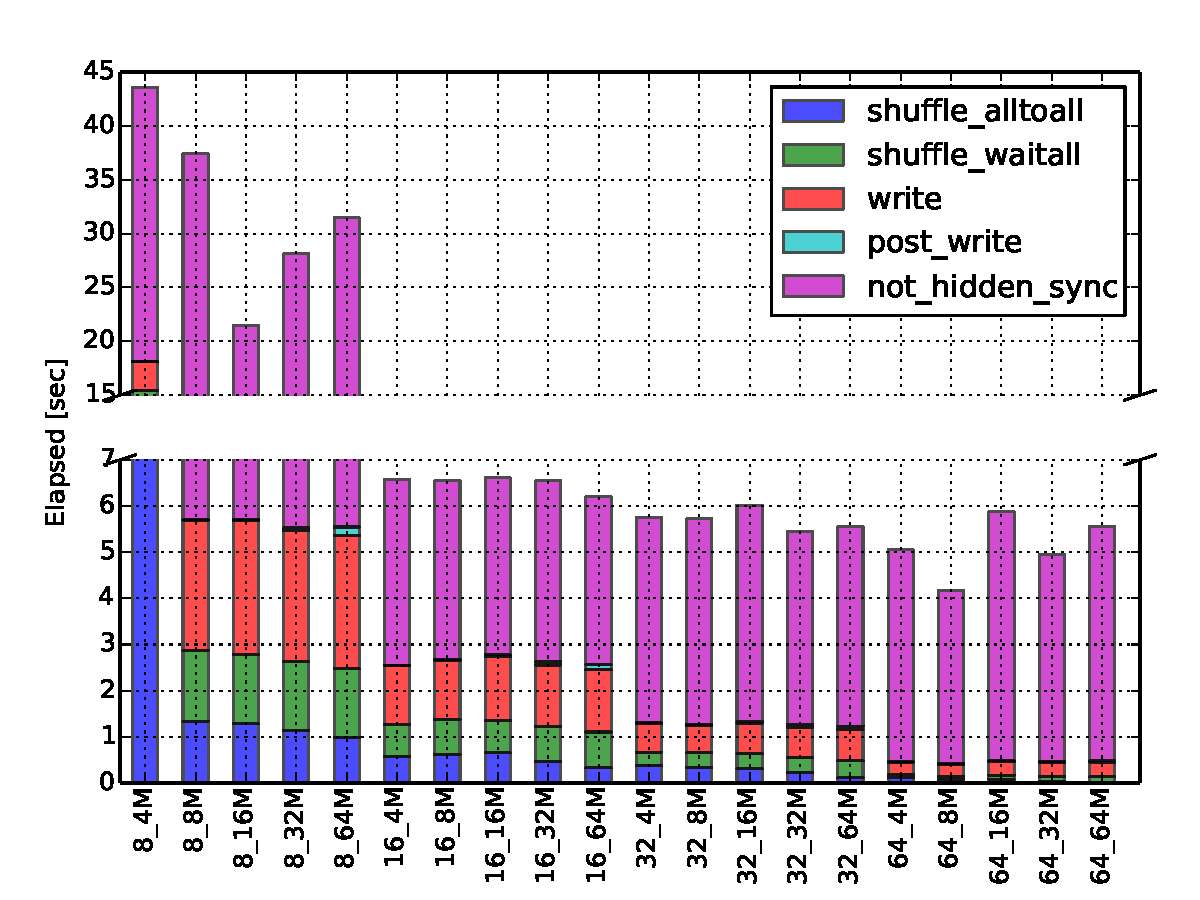
\includegraphics[width=0.95\columnwidth]{figures/ior_32GB_30sec_enable}
  \caption{IOR collective I/O contribution breakdown when cache is enabled.}
  \label{figure: ior-elaps-enable}
\end{figure}
In this figure we can clearly observe the not\_hidden\_sync term preventing IOR from achieving higher performance. This is added to the other time contributions and corresponds to the term $T_s(k)-C(k+1)$ reported in Equation~\ref{formula: bw}. In our specific case, $k = 4$ and $C(4+1) = 0,$ meaning that the total write time is accounting for the whole $T_s(4)$ term.


%\chapter{Evaluation} \label{chapt: evaluation}
In this chapter we present results for the Mercury middleware and the MPI-IO hints extensions for collective I/O proposed in previous chapters. For Mercury we consider a high energy physics code.
This application is representative of a class of HPC analysis applications that are becoming more and more common in workloads of leadership class systems. Our goal is to demonstrate that through
user guided I/O prefetching even a non-optimized application can improve its I/O utilization (and thus performance) of the file system.
For our ROMIO improvements we consider a range of collective I/O benchmarks that include synthetic and real application kernels. We run every benchmark with the baseline collective I/O implementation
in ROMIO and discuss in detail all the ext2ph performance implications; then we enable our NVM based optimization and show how the same performance implications can be mitigated or completely
cancelled when taking the global parallel file system out of the ext2ph critical I/O path.

\section{I/O Prefetching in ROOT}
Our target real world application is written using `ROOT', an object-oriented framework widely adopted in the experimental high energy physics community to build software 
for data analysis. The application runs on the Mogon cluster at the data processing center of the University of Mainz (ZDV), in Germany. It analyzes particle data read from 
an input file structure using the `ROOT' format (structured file format).

\begin{figure*}[!htb]
  \centering
  \begin{subfigure}[t]{0.7\textwidth}
    \centering
    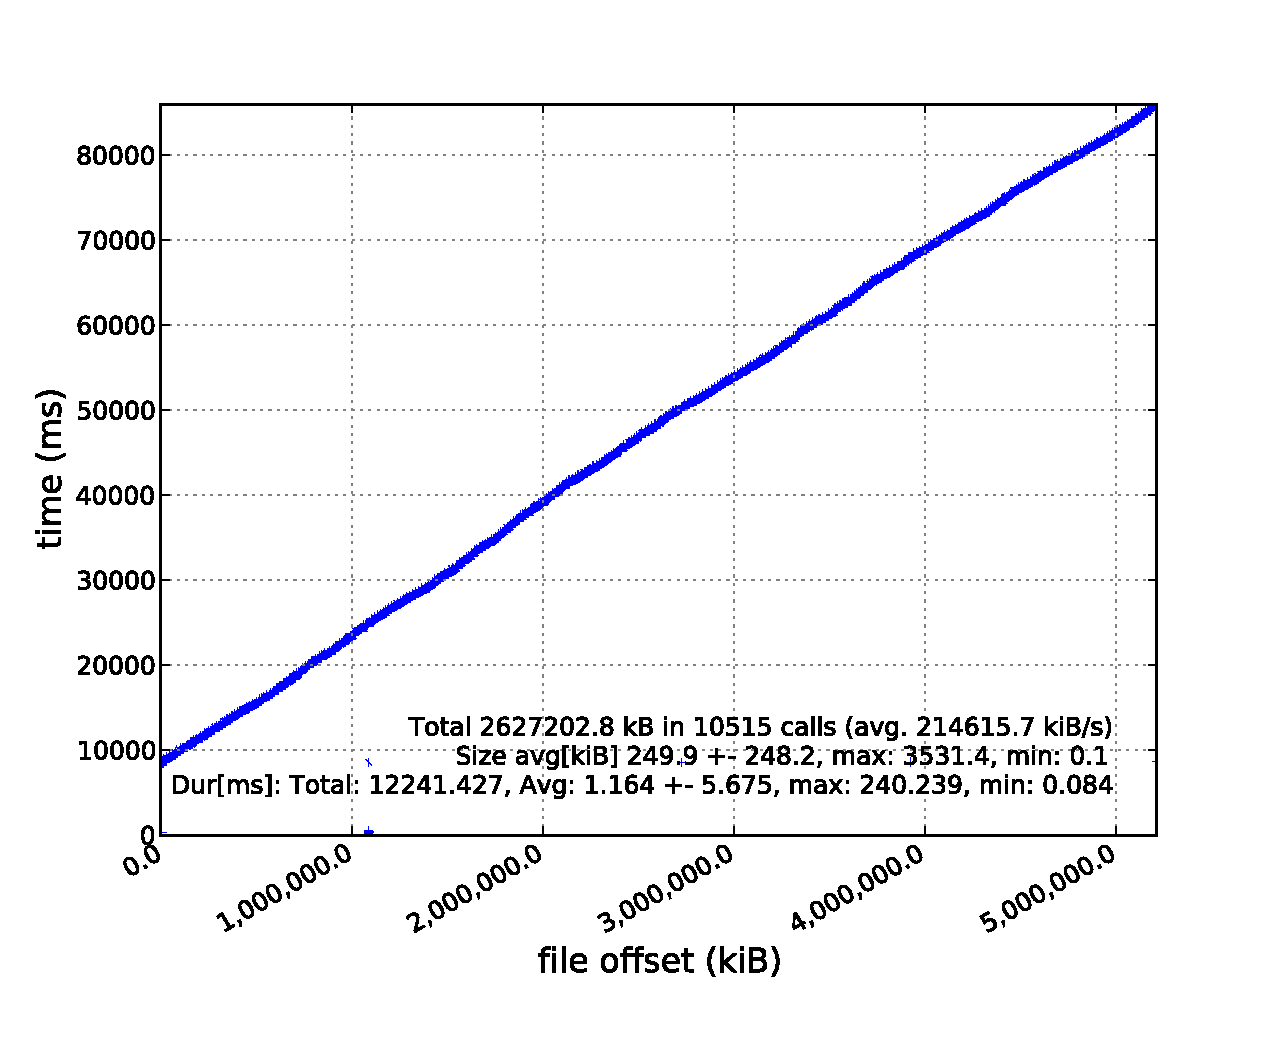
\includegraphics[width=\textwidth]{figures/iopat_profile}
    \caption{\textit{}}
    \label{figure: iopat_profile}
  \end{subfigure}
  \begin{subfigure}[t]{0.7\textwidth}
    \centering
    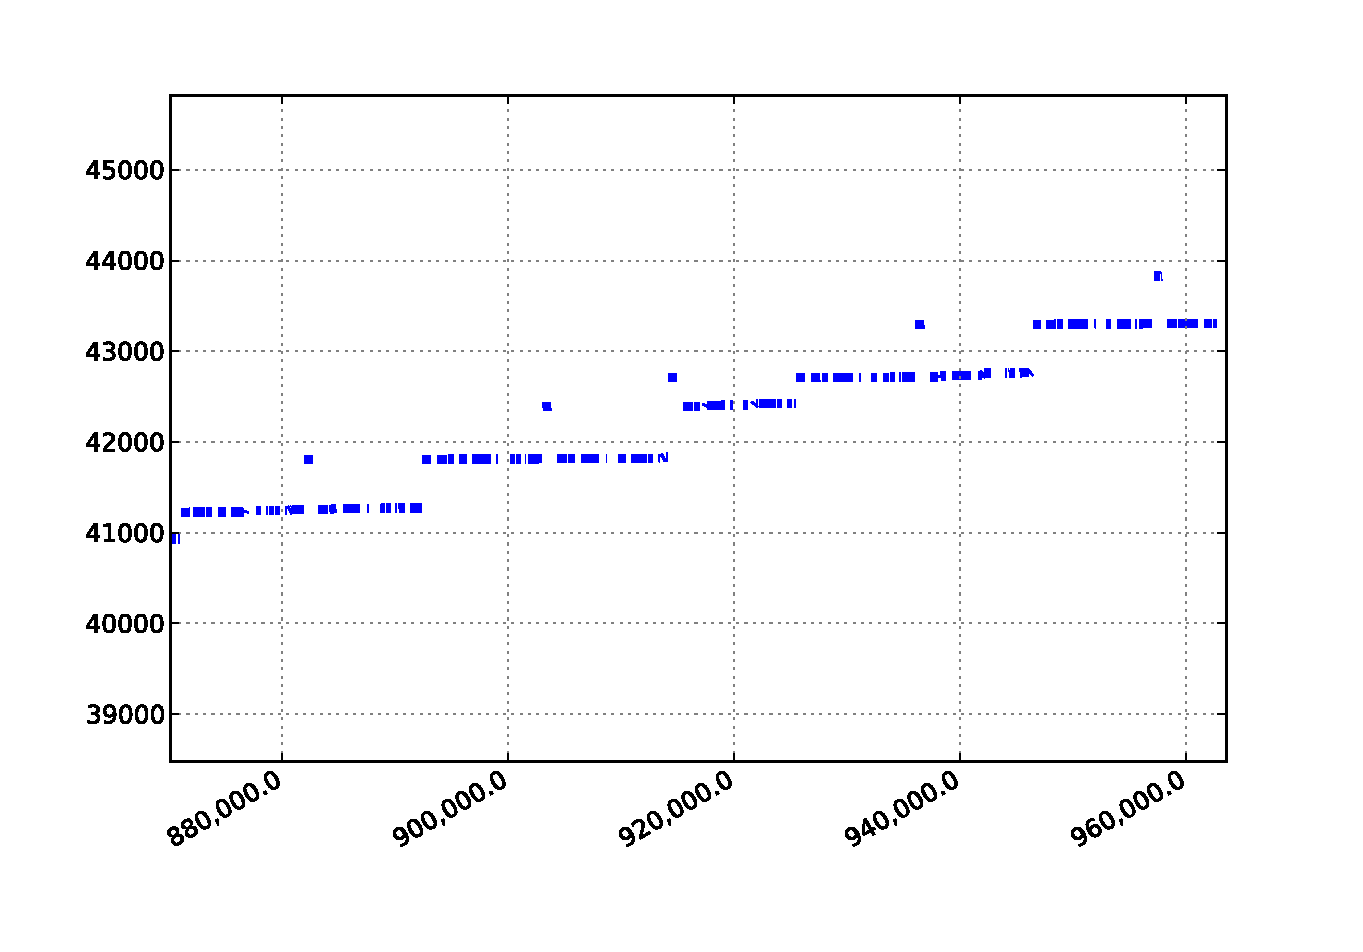
\includegraphics[width=\textwidth]{figures/00050_zoom}
    \caption{\textit{}}
    \label{figure: iopat_zoom}
  \end{subfigure}
  \caption{I/O read profile of the target application under analysis (\ref{figure: iopat_profile}), extracted from the the GPFS file system in the test cluster, and zoomed 
  window (\ref{figure: iopat_zoom}) showing the actual pattern details.}
  \label{figure: iopattern_with_statistics}
\end{figure*}

First of all we characterized the application's I/O pattern for a target file using traces and statistics extracted through several tools such as \textit{strace}, \textit{ioapps}\footnote{\url{https://code.google.com/p/ioapps}.} 
and GPFS's \textit{mmpmon} monitoring tool. 
Figure~\ref{figure: iopattern_with_statistics} shows the I/O pattern along with some additional statistics. As it can be seen, in this specific case (5 GB file), the application issues a total of 
10515 \texttt{read()} system calls to read about 2.6 GB of total data. The average request size is 250 KB and the time spent waiting for I/O is 12 seconds, when running on the test cluster. 

At a first glance the general I/O behaviour of the application looks sequential, most of the accesses to the file follow an increasing offset. Nevertheless, adjacent reads are separated by gaps 
(a strided read pattern). In a few cases this gap becomes negative, meaning that the application is moving backwards in the file to read some data previously left behind (as reported in 
Figure~\ref{figure: iopat_zoom}).

After a detailed I/O pattern analysis we could divide the target file into contiguous non-overlapping ranges. Within these ranges reads happen to have increasing offset. Even though the general 
I/O pattern of the application for different files looks similar\footnote{Due to space limits we do not report the comparison between different files.}, the size of the non-overlapping ranges may 
change significantly. This general behaviour can be modelled using Mercury through a configuration file in which a `WillNeed' hint covers the whole file from beginning to end (i.e., `Offset' and `Length' equal to 
0). The backwards seeks can be accounted for using the `CacheSize' parameter to keep previously accessed blocks in cache. In this way we effectively emulate a sliding window that tracks the application's 
I/O behaviour. This would not be possible by just using a, e.g., \texttt{POSIX\_FADV\_WILLNEED} advice on the whole file before starting the application like shown by Figure~\ref{figure: fadvise_comparison}. 
The reason is that even if the file fits entirely into the cache, we would have a large number of valuable pages, possibly from other applications, discarded from the cache to load data that will be accessed at the end of 
the application. Additionally, if the file size is bigger than the cache size we would have the file system discarding blocks at the beginning of the file as the blocks at the end are preloaded, 
effectively forcing the application to access these blocks from the I/O servers instead of the cache. With our approach, on the other hand, we keep in the cache only a small, controlled number of 
blocks (the ones currently accessed), while the older blocks are discarded since no longer needed.

\begin{figure}[!htb]
  \centering
  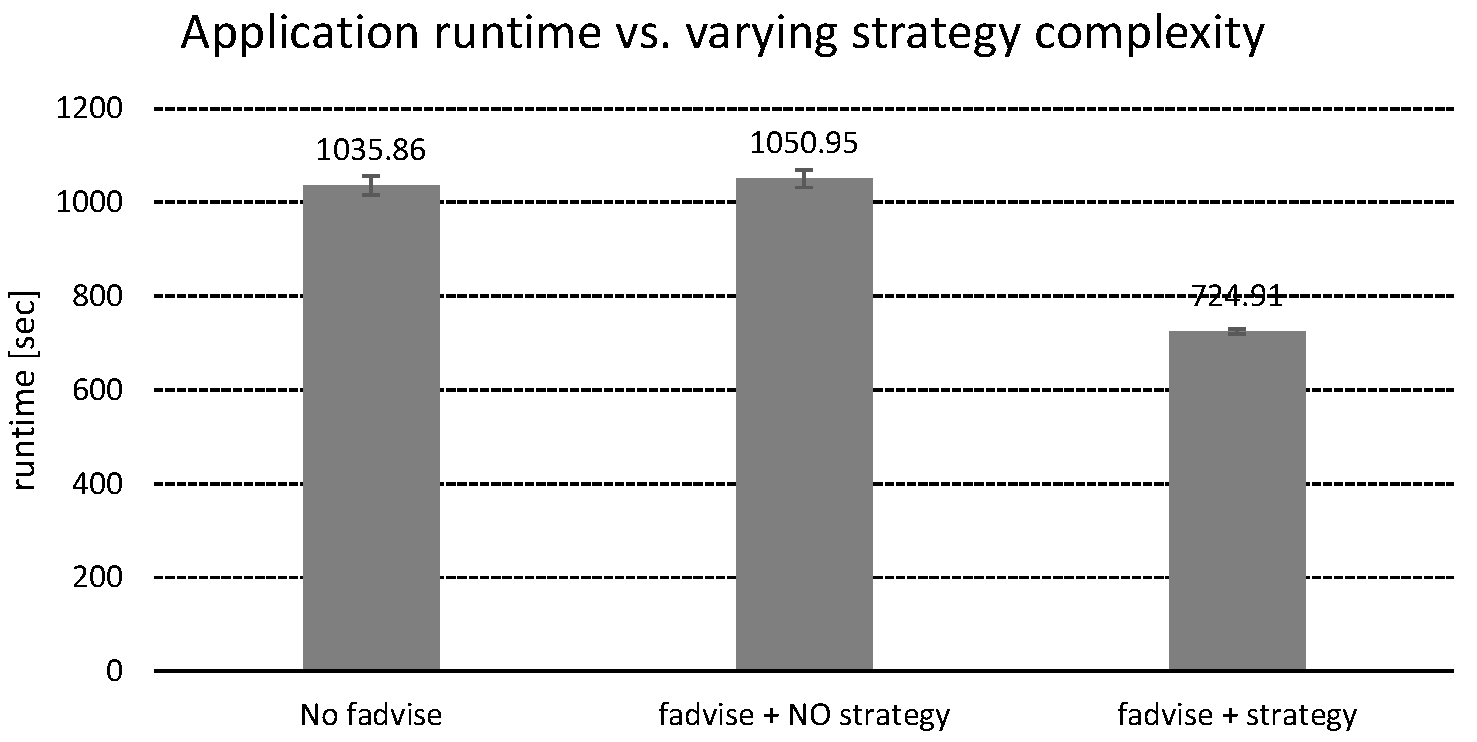
\includegraphics[width=0.8\textwidth]{figures/test_fadvise_no_border}
  \caption{Comparison between different usage stategies of posix\_fadvise for an input file of 55 GB residing in an ext4 file system. The first bar represents the case in which no advice is used, 
  the second bar represents the case in which a POSIX\_FADV\_WILLNEED is issued for the whole file at the beginning of the application and the third bar represents the case in which POSIX\_FADV\_WILLNEED 
  is issued using Mercury.}
  \label{figure: fadvise_comparison}
\end{figure} 

To assess the impact of our Mercury prototype on the application and file systems performance we considered the application execution time and the number of reads accounted for by the respective file systems. 
We conducted our experiments without file system hints and then with file system hints issued transparently to the application by the \textit{Advice Manager}. Furthermore, we ran each experiment three 
times and calculated average, minima and maxima for each metric. In order to avoid caching affecting our measurements, extra care was taken to clean all the relevant caches for the different file systems. 
For ext4 and Lustre this was accomplished by using the command line: $$echo\ 3 > /proc/sys/vm/drop\_caches$$ on the file system clients. Additionally, for Lustre this command was also executed on the
\textit{object storage servers} (OSSs) to avoid the server side cache to be retained. In the case of GPFS, the file system client's page pool was cleaned using the clean file cache hint in Table~\ref{table: hints_table}, 
the GPFS \textit{network shared disks} (NSDs)\footnote{GPFS name for I/O servers.} servers do not cache any data. 


\subsection{Testbed}
Our testbed is composed by a test cluster of seven nodes, mainly intended to evaluate the proposed Linux kernel modifications with the Lustre file system. The reason 
for using a smaller cluster instead of the Mogon system is that it was not possible to disrupt the production cluster, affecting hundreds of users, by re-installing 
the operating system kernel. In order to make realistic comparisons between Lustre and GPFS, the test cluster also has a GPFS file system on comparable hardware. 

Both file systems have a single disk server each, one Dell R710 acts as GPFS network shared disk (NSD) server and another as Lustre object storage server. The R710 are equipped 
with two quadcore E5620 @2.4 GHz and 24 GB main memory. For storage, both disk servers share a MD3200 array with 2 controllers and 4 MD1200 expansion shelves for a total 
of 60 2 TB drives. The Storage is formatted in 4 15 dynamic disk pools. This is the LSI/Netapp type of declustered RAID, which distributes the 8+2 RAID6 stripes evenly 
over all 15 disks for better rebuild performance. The disk block size is set to 128 KB, which results in a RAID stripe size of 1 MB. The four disk pools are then split 
on the Array into LUNs, one of the LUNs from each disk pool is then used for GPFS and another one from each pool is used for Lustre. This results in comparable resources 
for both file systems and tests do not interfere with each other, as long as only one file system is tested at a time. 

While the GPFS filesystem embeds the metadata with the data, Lustre needs a separate Metadata Server (MDS). This is hosted by a SuperMicro server equipped with one quadcore Xeon 
E3-1230 @3.3 GHz and 16 GB of main memory, as metadata target (MDT) it uses a 120 GB SSD Intel 520. Four other machines of the same type, equipped with an eight core E3-1230 @3.3 
GHz processor and 16 GB of main memory, work as compute nodes and file system clients. All machines, servers and clients, are equipped with Intel X520DA 10 Gigabit adapters and 
connected to a SuperMicro SSE-X24S 24 ports 10 Gigabit switch. Both, the GPFS and Lustre file systems are formatted with a block size of 4 MB.

\subsection{Performance Results}
To measure the performance improvements that our Mercury prototype can deliver to the application's run-time we conducted two set of tests. In the first test we varied the size of the input file from 5 to 95 GB. 
This is mainly aimed to study the behaviour of the `ROOT' application using different input file sizes and how our solution behaves when the file becomes bigger than the available cache space. In the second 
test we varied the number of `ROOT' instances running simultaneously from 1 to 8. By doing so we study the interaction of multiple processes accessing the file system and how these can benefit from the prefetching 
hints generated by Mercury. Figures~\ref{figure: run-time_1} and~\ref{figure: run-time_2} report the results for the described experiments. All the tests where performed using a `BlockSize' of 4 MB, a `CacheSize' of 
8 blocks, a `ReadAheadSize' of 4 blocks, and a `WillNeed' hint covering the whole file (i.e., with `Offset' and `Length' equal to 0), resulting in each process consuming up to 32 MB of cache space and 512 MB in total 
for 8 application instances. 

The `WillNeed' on the whole file causes the \textit{Advisor Thread} to issue up to 4 (`ReadAheadSize') prefetching requests for blocks of 4 MB sequentially, starting from the current accessed 
block. This has the same effect of data sieving in ROMIO, optimizing the access size and allowing the application to read the requested data randomly from the cache instead of the file system. The produced effect is 
particularly beneficial in the case of Lustre and ext4, as it can be seen in Figures~\ref{figure: ext4_1} and~\ref{figure: lustre_1}. In these cases we measure reductions in the execution time of up to 50\%, with respect 
to the normal case. For GPFS we can still observe an improvement, but this is more contained compared to the other file systems (Figure~\ref{figure: gpfs_1}). The reductions in the execution time measured in GPFS are on 
average up to 10\%, with respect to the normal case. The reason is that the default prefetching strategy in GPFS works better that traditional read-ahead. In fact, by disabling the prefetching in GPFS we observed reductions 
in the execution time comparable to the other file systems (not reported here).

%\begin{figure}[!htb]
%  \centering
%  \begin{subfigure}[t]{0.48\textwidth}
%    \centering
%    \includegraphics[width=\textwidth]{figures/ext4/runtime}
%    \caption{\textit{}}
%    \label{figure: ext4_1}
%  \end{subfigure}
%  \begin{subfigure}[t]{0.48\textwidth}
%    \centering
%    \includegraphics[width=\textwidth]{figures/gpfs/runtime}
%    \caption{\textit{}}
%    \label{figure: gpfs_1}
%  \end{subfigure}
%  \begin{subfigure}[t]{0.48\textwidth}
%    \centering
%    \includegraphics[width=\textwidth]{figures/Lustre/runtime}
%    \caption{\textit{}}
%    \label{figure: lustre_1}
%  \end{subfigure}
%  \caption{Running time of the ROOT application for the three file systems under study using different input file sized (\ref{figure: ext4_1},~\ref{figure: gpfs_1} and~\ref{figure: lustre_1}).}
%  \label{figure: run-time_1}
%\end{figure}
%
%\begin{figure}[!htb]
%  \centering
%  \begin{subfigure}[b]{0.48\textwidth}
%    \centering
%    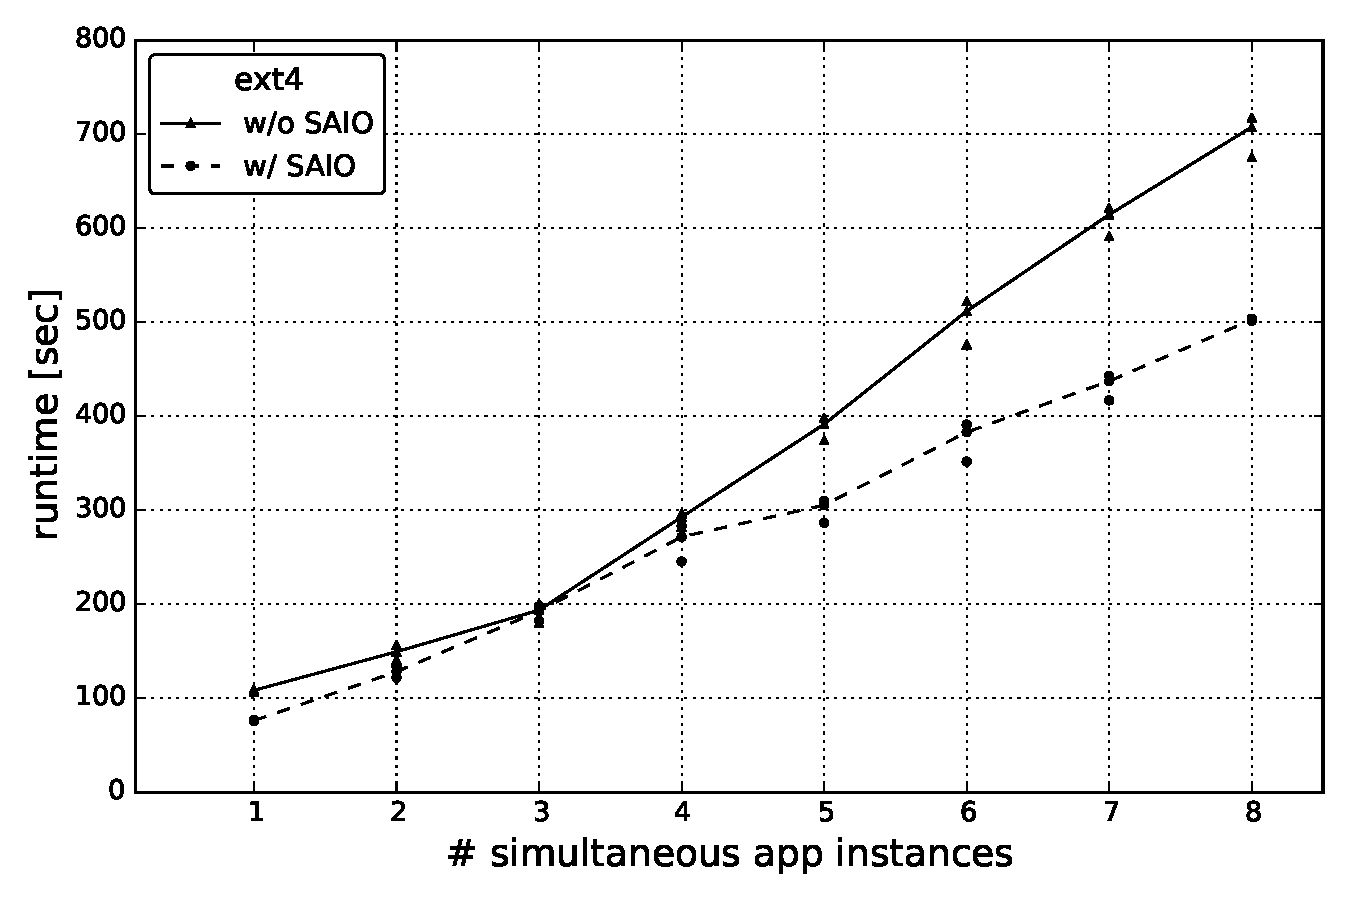
\includegraphics[width=\textwidth]{figures/simult_instance_ext4_test_cluster}
%    \caption{\textit{}}
%    \label{figure: ext4_2}
%  \end{subfigure}
%  \begin{subfigure}[b]{0.48\textwidth}
%    \centering
%    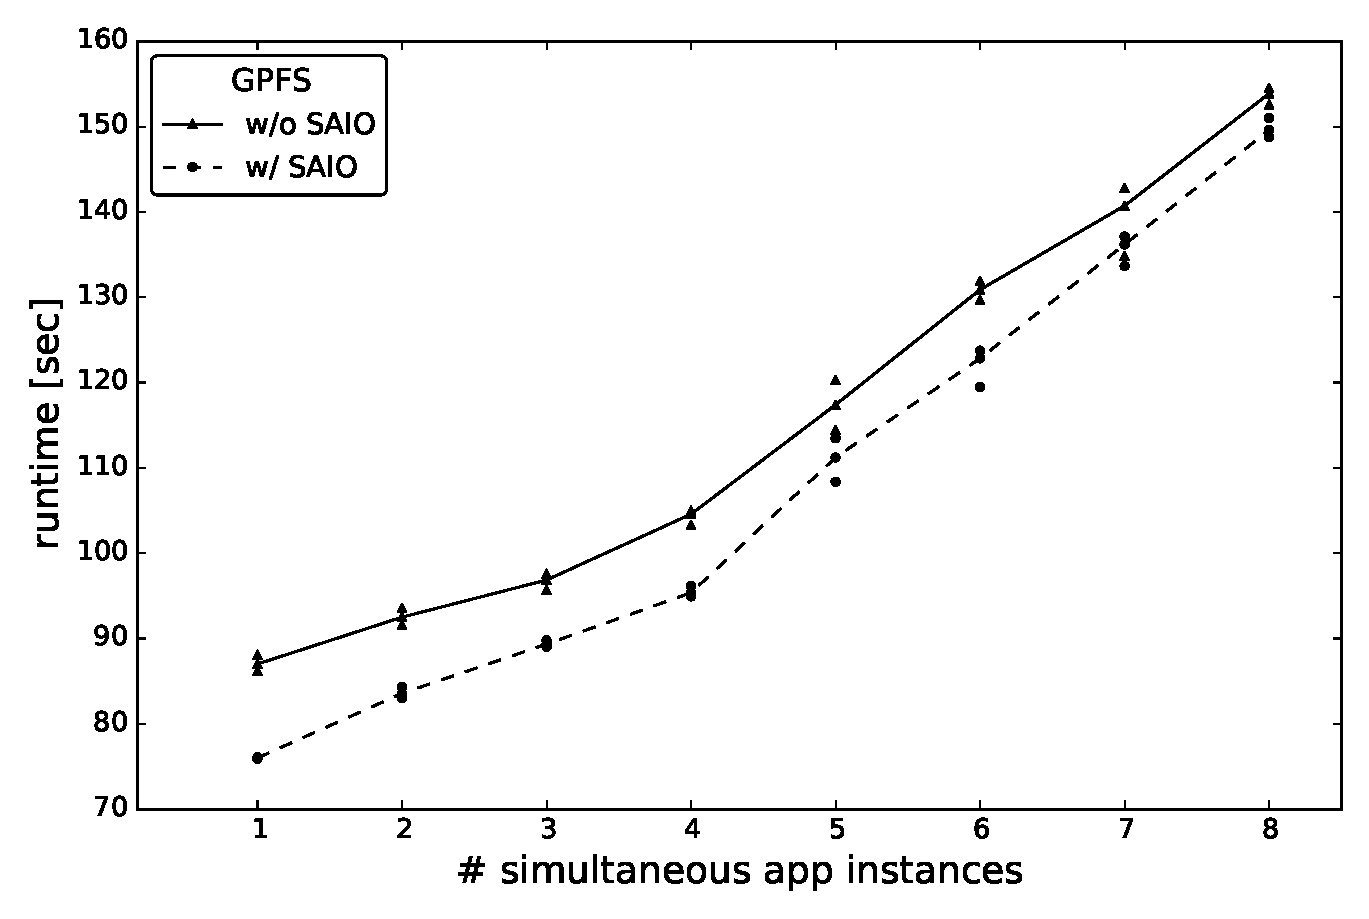
\includegraphics[width=\textwidth]{figures/simult_instance_gpfs_test_cluster}
%    \caption{\textit{}}
%    \label{figure: gpfs_2}
%  \end{subfigure}
%  \begin{subfigure}[b]{0.48\textwidth}
%    \centering
%    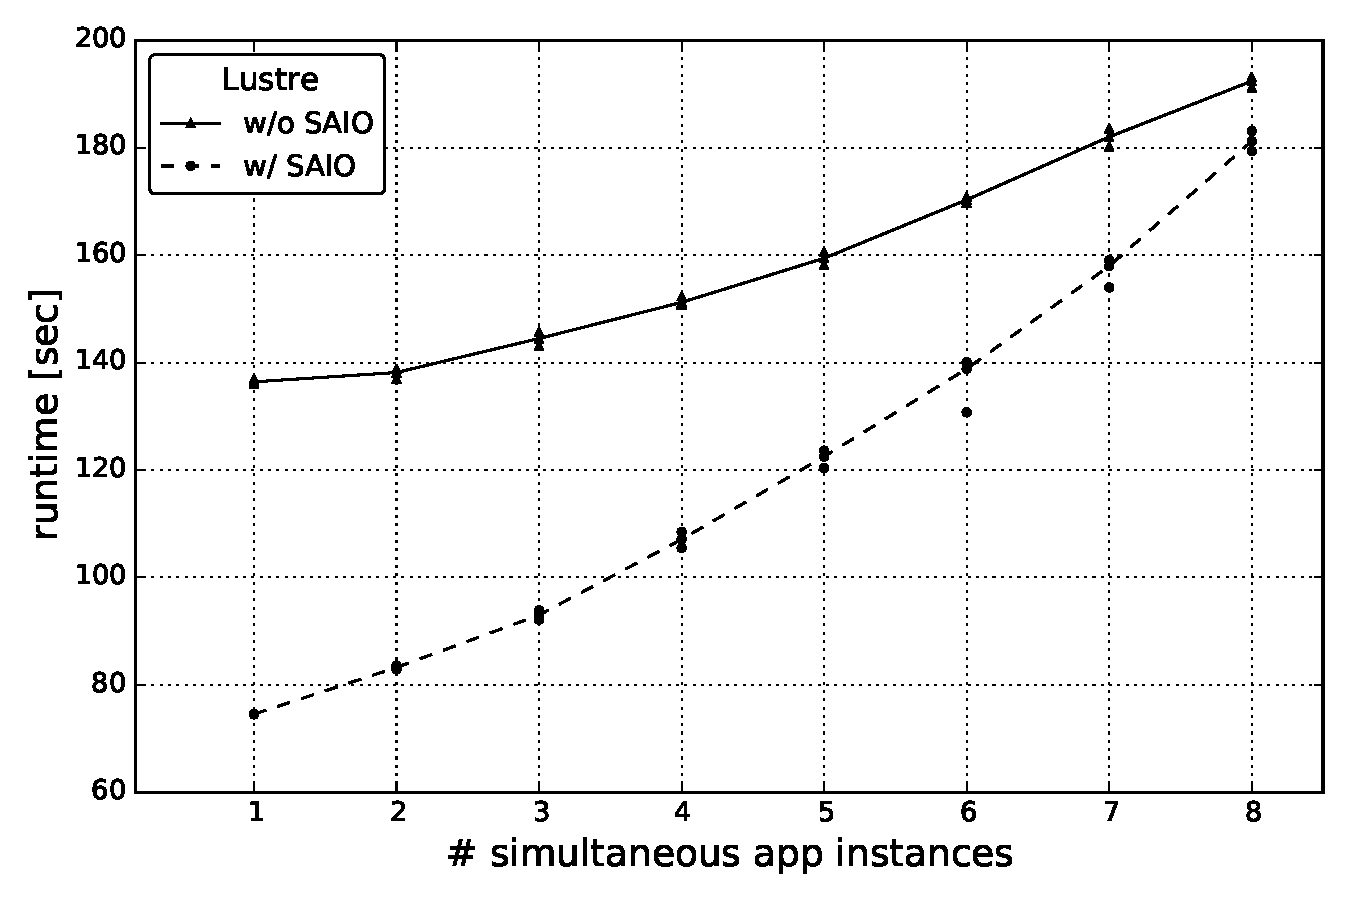
\includegraphics[width=\textwidth]{figures/multiple_simult_procs_Lustre_testcluster}
%    \caption{\textit{}}
%    \label{figure: lustre_2}
%  \end{subfigure}
%  \caption{Running time of the ROOT application for the three file system under study using different of application instances accessing a file of 5 GB (\ref{figure: ext4_2},~\ref{figure: gpfs_2} and~\ref{figure: lustre_2}).}
%  \label{figure: run-time_2}
%\end{figure}
%
%\begin{figure}[!htb]
%  \centering
%  \begin{subfigure}[t]{0.48\textwidth}
%    \centering
%    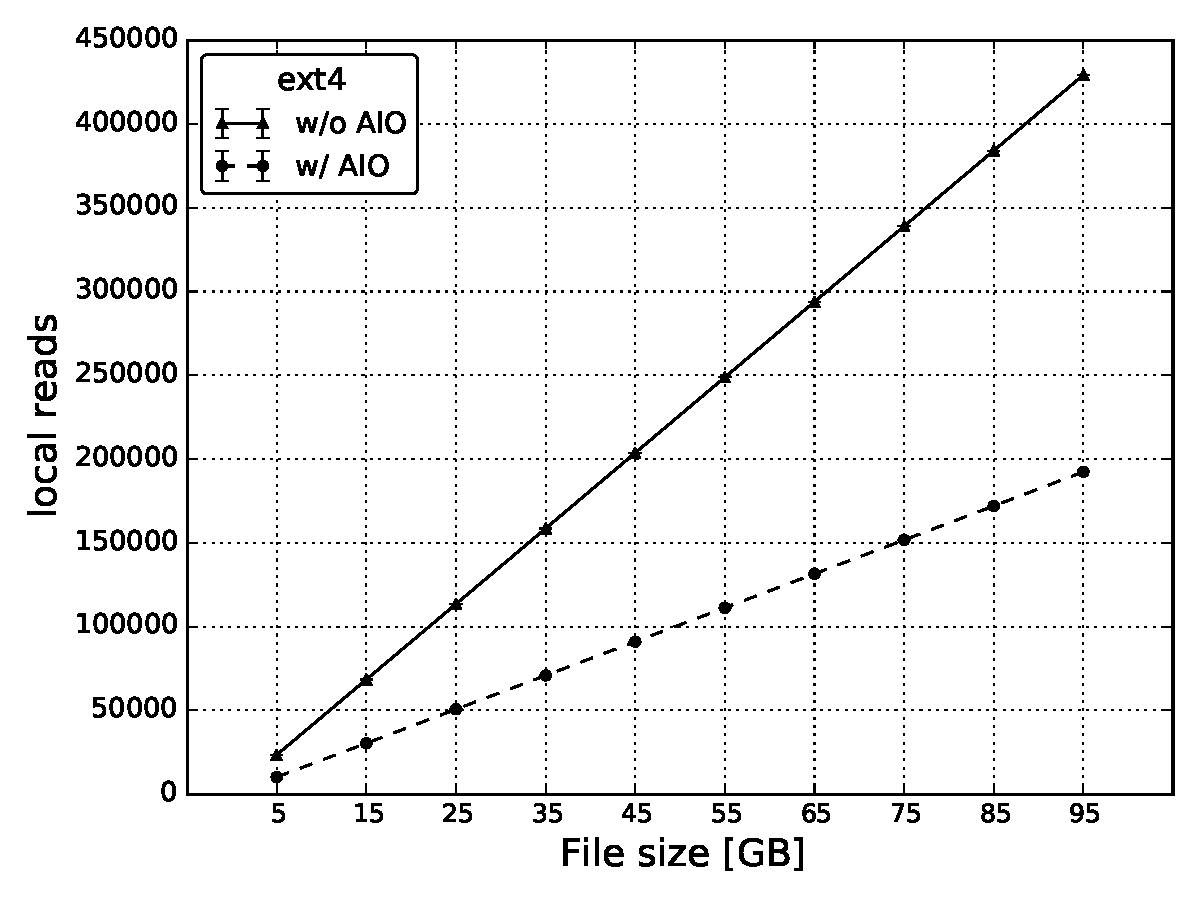
\includegraphics[width=\textwidth]{figures/ext4/reads}
%    \caption{\textit{}}
%    \label{figure: ext4_3}
%  \end{subfigure}
%  \begin{subfigure}[t]{0.48\textwidth}
%    \centering
%    \includegraphics[width=\textwidth]{figures/gpfs/server_reads}
%    \caption{\textit{}}
%    \label{figure: gpfs_3}
%  \end{subfigure}
%  \begin{subfigure}[t]{0.48\textwidth}
%    \centering
%    \includegraphics[width=\textwidth]{figures/Lustre/server_reads}
%    \caption{\textit{}}
%    \label{figure: lustre_3}
%  \end{subfigure}
%  \caption{Reads processed by local ext4, GPFS and Lustre I/O servers for various input file sizes (\ref{figure: ext4_3},~\ref{figure: gpfs_3} and~\ref{figure: lustre_3}).}
%  \label{figure: read_1}
%\end{figure}
%
%\begin{figure}[!htb]
%  \centering
%  \begin{subfigure}[b]{0.48\textwidth}
%    \centering
%    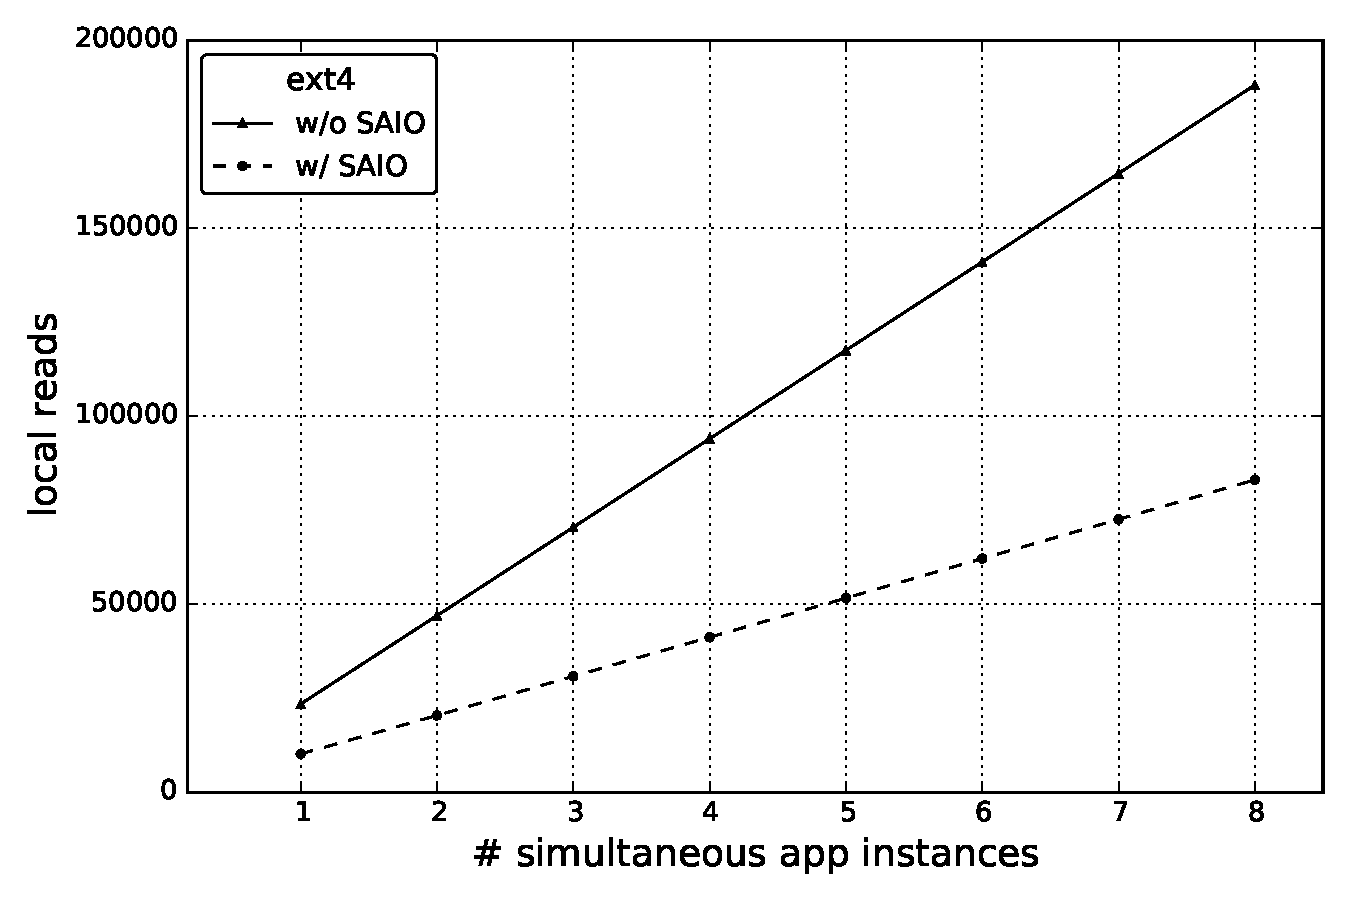
\includegraphics[width=\textwidth]{figures/reads_simult_instance_ext4_test_cluster}
%    \caption{\textit{}}
%    \label{figure: ext4_4}
%  \end{subfigure}
%  \begin{subfigure}[b]{0.48\textwidth}
%    \centering
%    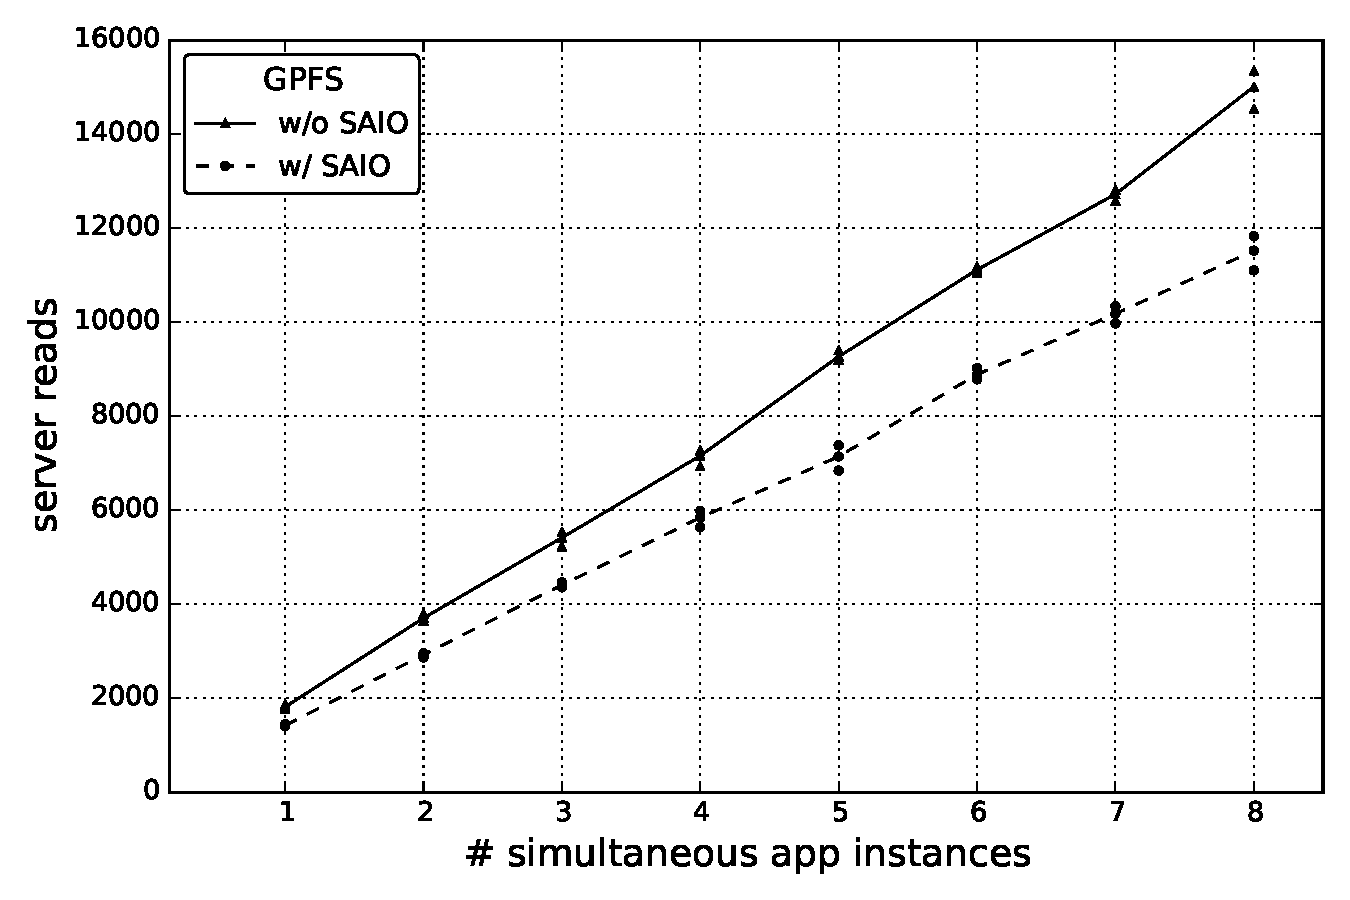
\includegraphics[width=\textwidth]{figures/reads_simult_instance_gpfs_test_cluster}
%    \caption{\textit{}}
%    \label{figure: gpfs_4}
%  \end{subfigure}
%  \begin{subfigure}[b]{0.48\textwidth}
%    \centering
%    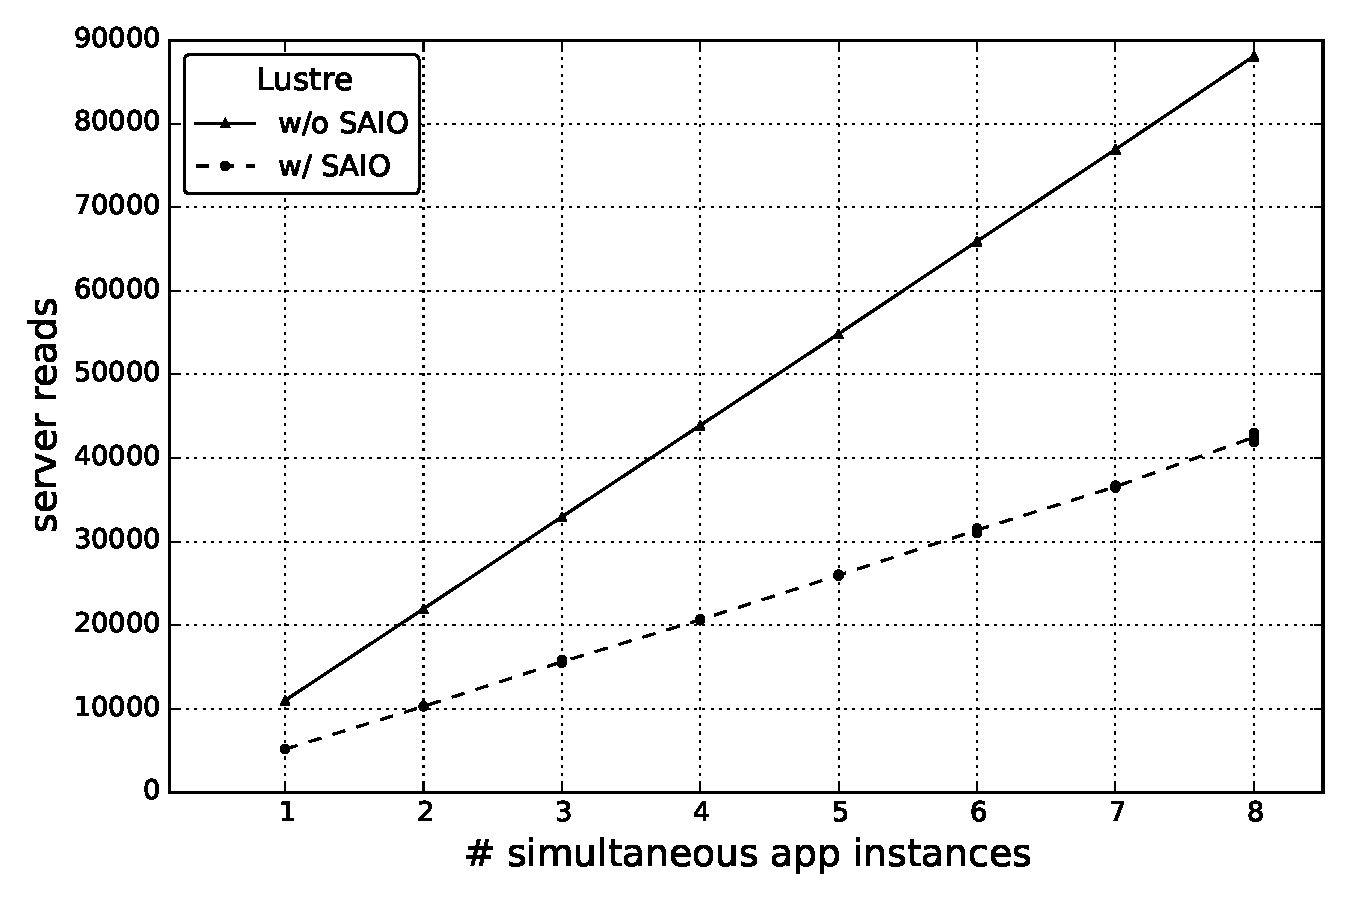
\includegraphics[width=\textwidth]{figures/reads_multiple_simult_procs_Lustre_testcluster}
%    \caption{\textit{}}
%    \label{figure: lustre_4}
%  \end{subfigure}
%  \caption{Reads processed by local ext4, GPFS and Lustre I/O servers for multiple instances of ROOT accessing a file of 5 GB (\ref{figure: ext4_4},~\ref{figure: gpfs_4} and~\ref{figure: lustre_4}).}
%  \label{figure: read_2}
%\end{figure}

\begin{figure*}[]
  \centering
  \begin{subfigure}[]{0.70\textwidth}
    \centering
    \includegraphics[width=\textwidth]{figures/ext4/runtime}
    \caption{\textit{}}
    \label{figure: ext4_1}
  \end{subfigure}
  \begin{subfigure}[]{0.70\textwidth}
    \centering
    \includegraphics[width=\textwidth]{figures/gpfs/runtime}
    \caption{\textit{}}
    \label{figure: gpfs_1}
  \end{subfigure}
  \begin{subfigure}[]{0.70\textwidth}
    \centering
    \includegraphics[width=\textwidth]{figures/Lustre/runtime}
    \caption{\textit{}}
    \label{figure: lustre_1}
  \end{subfigure}
  \caption{Running time of the ROOT application for the three file systems under study using different input file sized (\ref{figure: ext4_1},~\ref{figure: gpfs_1} and~\ref{figure: lustre_1}).}
  \label{figure: run-time_1}
\end{figure*}

\begin{figure*}[]
  \centering
  \begin{subfigure}[]{0.70\textwidth}
    \centering
    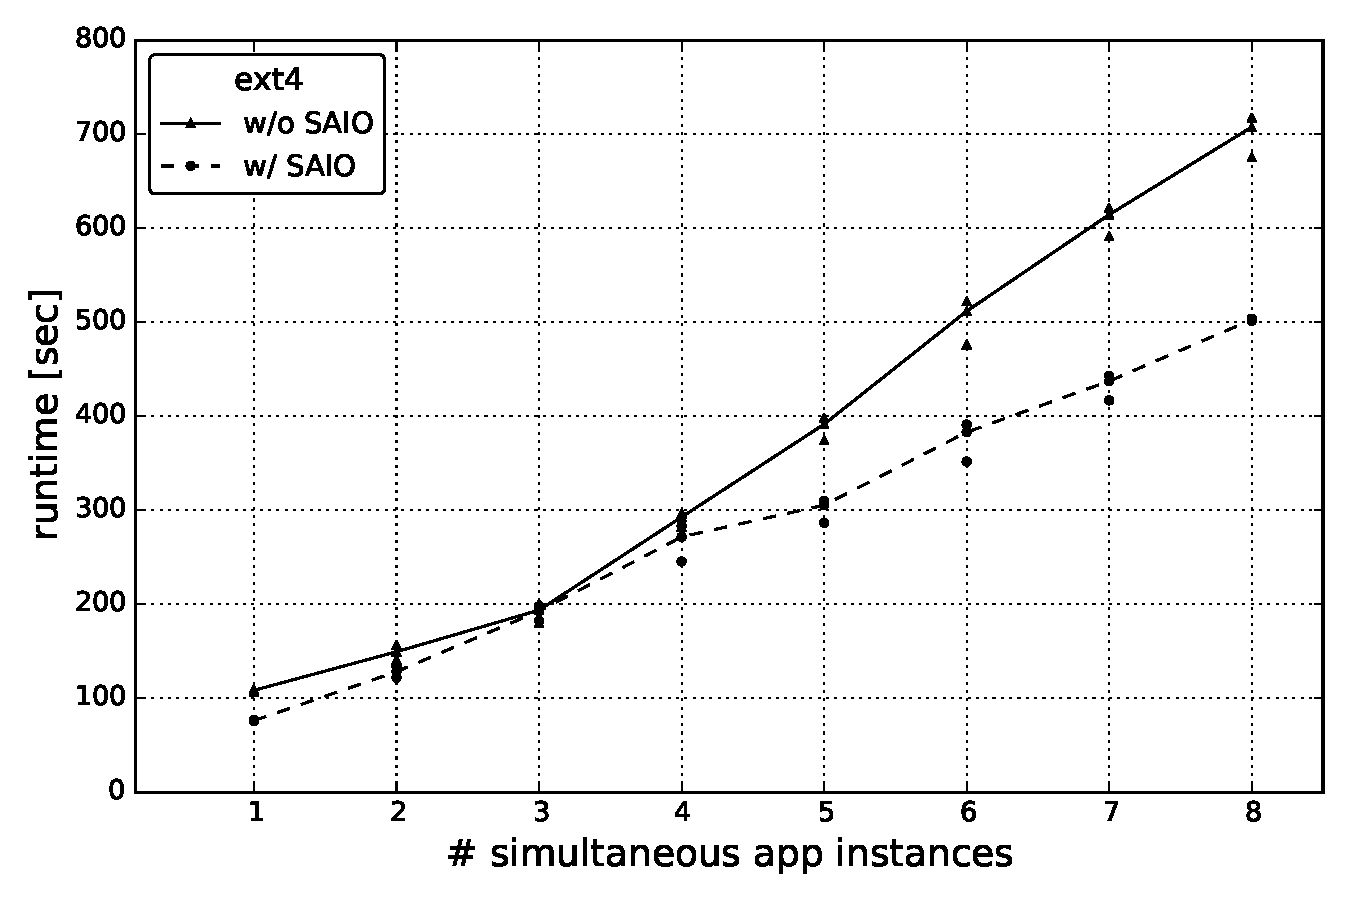
\includegraphics[width=\textwidth]{figures/simult_instance_ext4_test_cluster}
    \caption{\textit{}}
    \label{figure: ext4_2}
  \end{subfigure}
  \begin{subfigure}[]{0.70\textwidth}
    \centering
    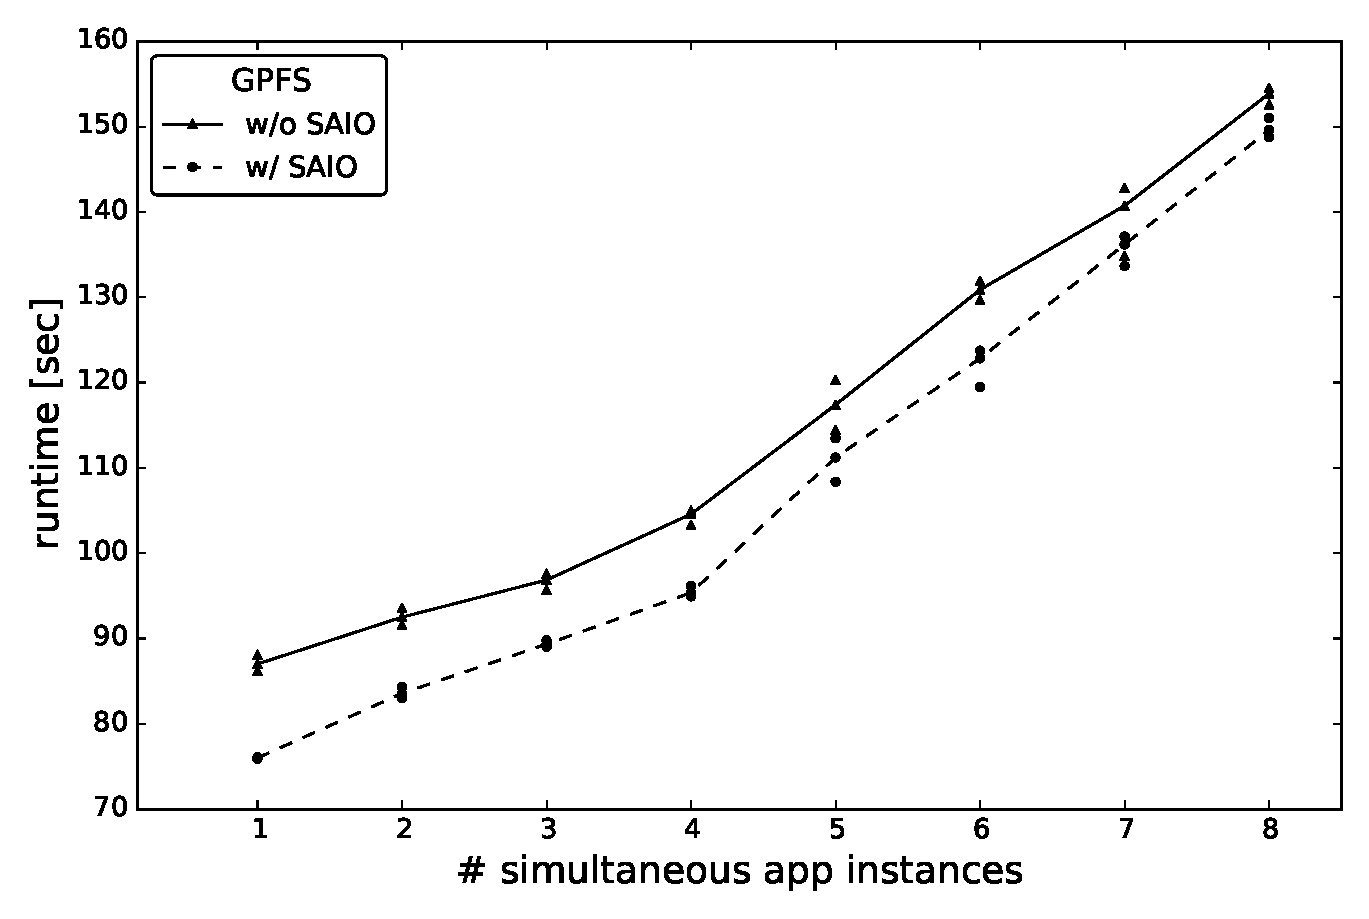
\includegraphics[width=\textwidth]{figures/simult_instance_gpfs_test_cluster}
    \caption{\textit{}}
    \label{figure: gpfs_2}
  \end{subfigure}
  \begin{subfigure}[]{0.70\textwidth}
    \centering
    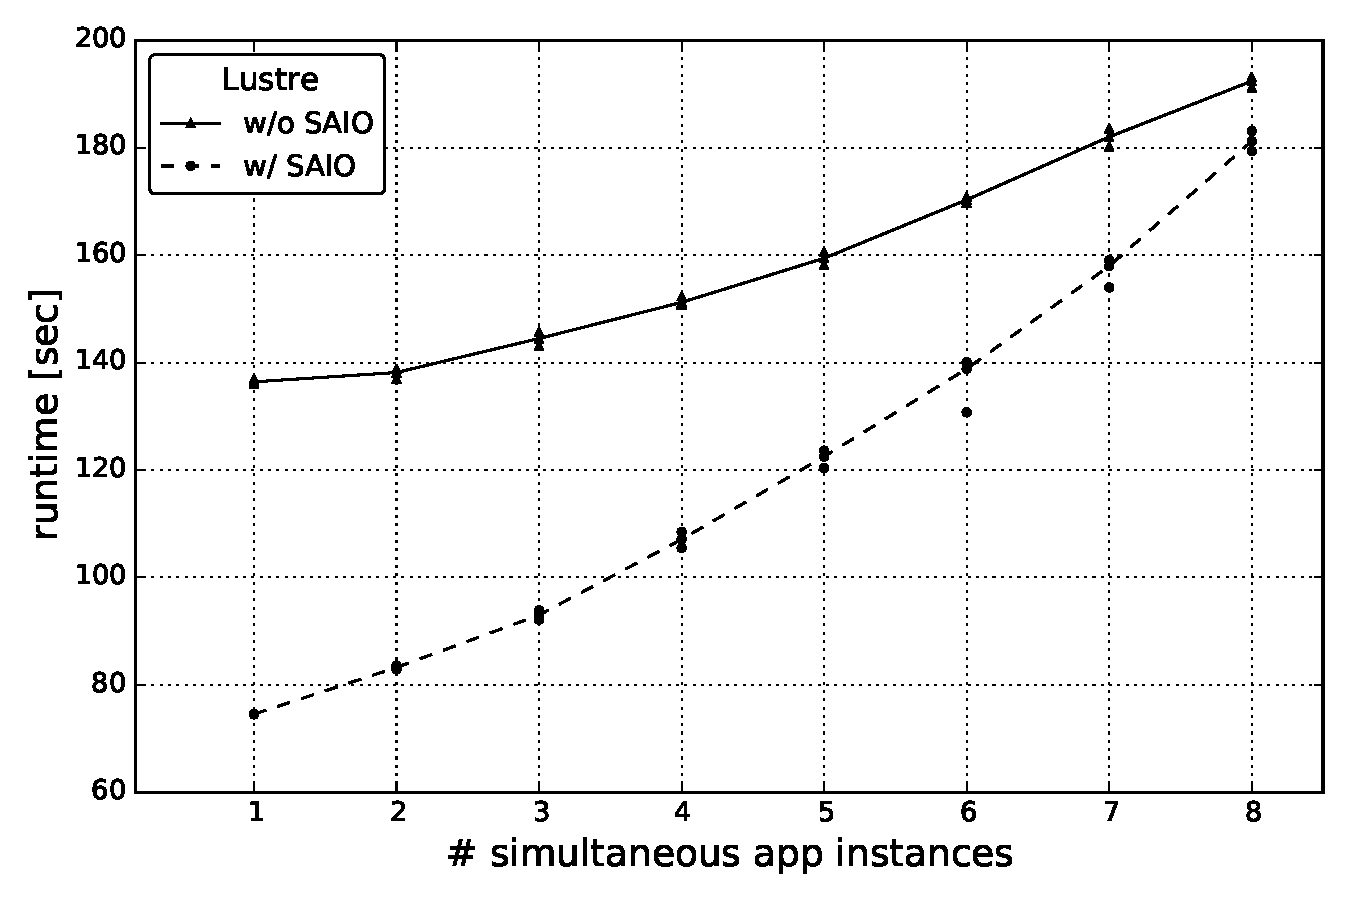
\includegraphics[width=\textwidth]{figures/multiple_simult_procs_Lustre_testcluster}
    \caption{\textit{}}
    \label{figure: lustre_2}
  \end{subfigure}
  \caption{Running time of the ROOT application for the three file system under study using different of application instances accessing a file of 5 GB (\ref{figure: ext4_2},~\ref{figure: gpfs_2} and~\ref{figure: lustre_2}).}
  \label{figure: run-time_2}
\end{figure*}

\begin{figure*}[]
  \centering
  \begin{subfigure}[]{0.70\textwidth}
    \centering
    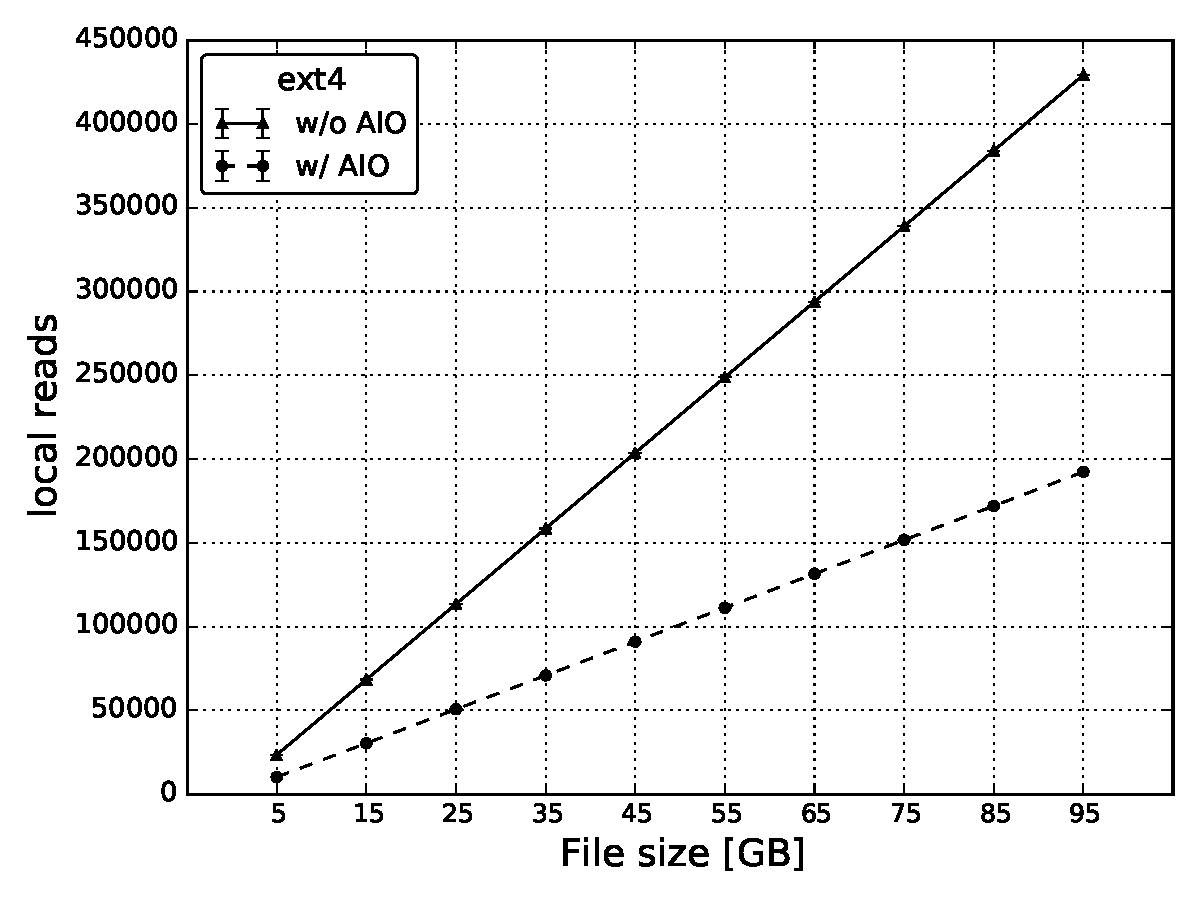
\includegraphics[width=\textwidth]{figures/ext4/reads}
    \caption{\textit{}}
    \label{figure: ext4_3}
  \end{subfigure}
  \begin{subfigure}[]{0.70\textwidth}
    \centering
    \includegraphics[width=\textwidth]{figures/gpfs/server_reads}
    \caption{\textit{}}
    \label{figure: gpfs_3}
  \end{subfigure}
  \begin{subfigure}[]{0.70\textwidth}
    \centering
    \includegraphics[width=\textwidth]{figures/Lustre/server_reads}
    \caption{\textit{}}
    \label{figure: lustre_3}
  \end{subfigure}
  \caption{Reads processed by local ext4, GPFS and Lustre I/O servers for various input file sizes (\ref{figure: ext4_3},~\ref{figure: gpfs_3} and~\ref{figure: lustre_3}).}
  \label{figure: read_1}
\end{figure*}

\begin{figure*}[]
  \centering
  \begin{subfigure}[]{0.70\textwidth}
    \centering
    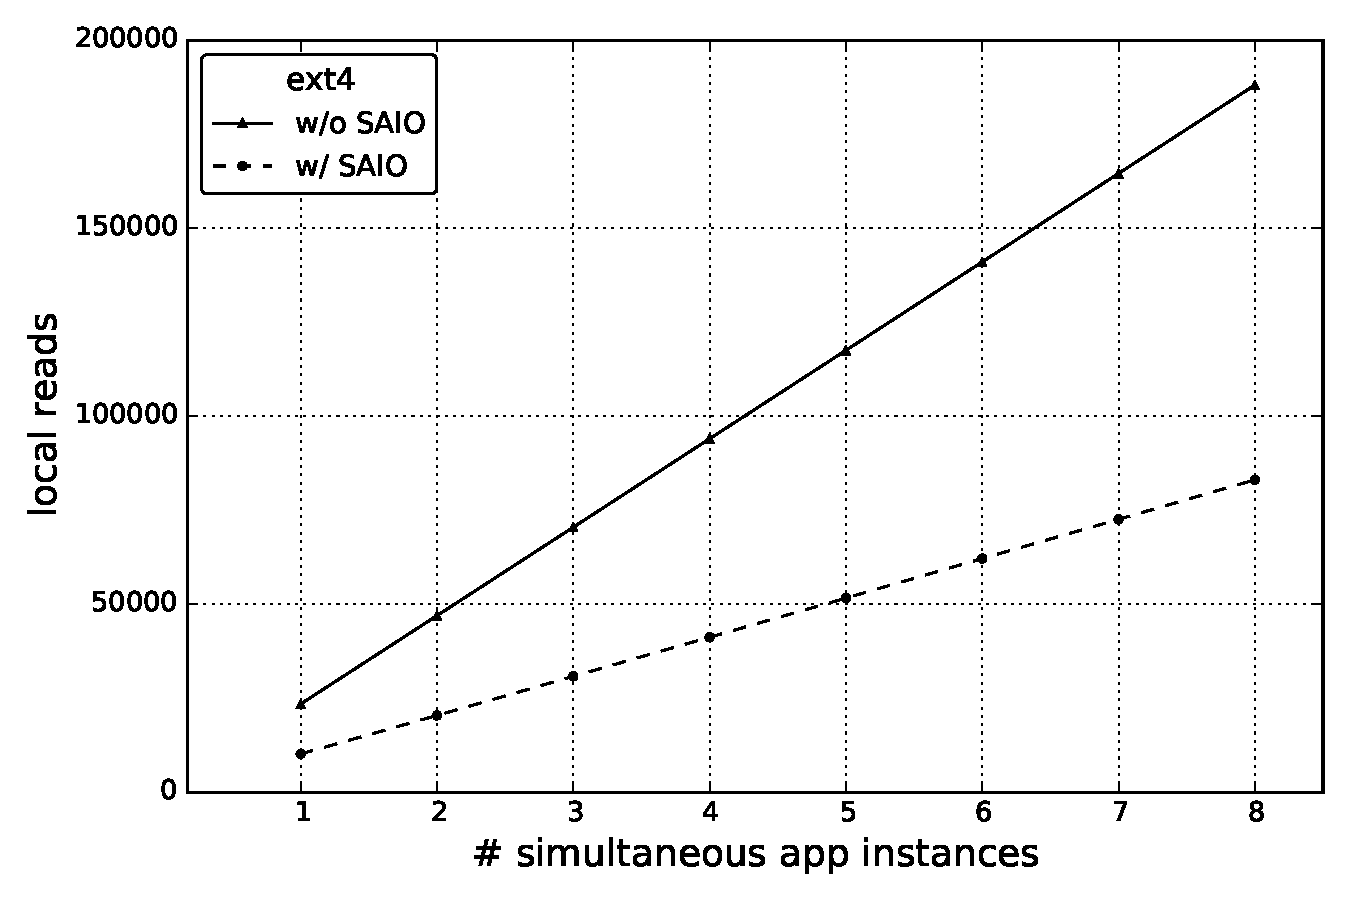
\includegraphics[width=\textwidth]{figures/reads_simult_instance_ext4_test_cluster}
    \caption{\textit{}}
    \label{figure: ext4_4}
  \end{subfigure}
  \begin{subfigure}[]{0.70\textwidth}
    \centering
    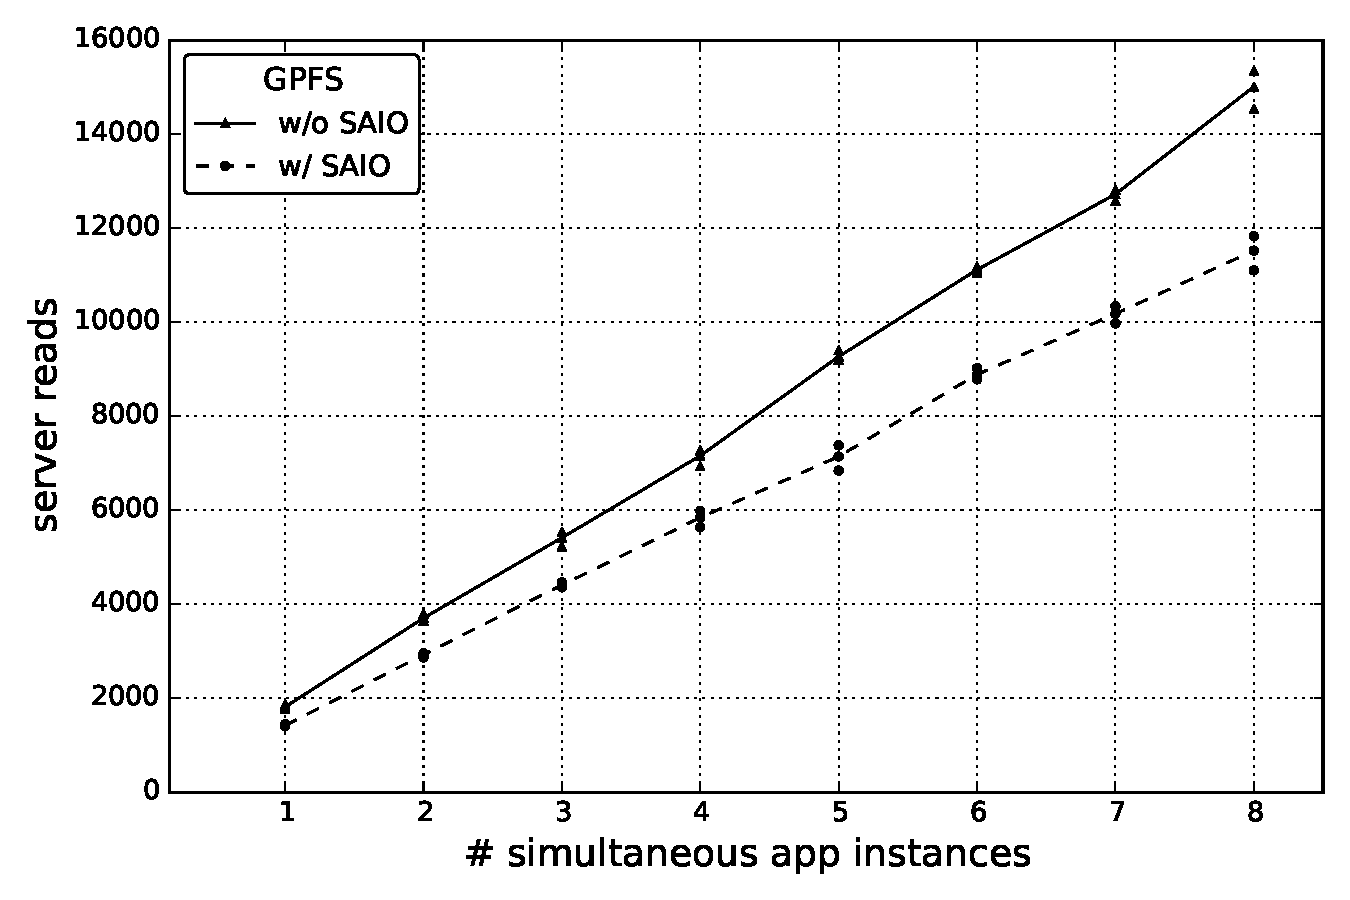
\includegraphics[width=\textwidth]{figures/reads_simult_instance_gpfs_test_cluster}
    \caption{\textit{}}
    \label{figure: gpfs_4}
  \end{subfigure}
  \begin{subfigure}[]{0.70\textwidth}
    \centering
    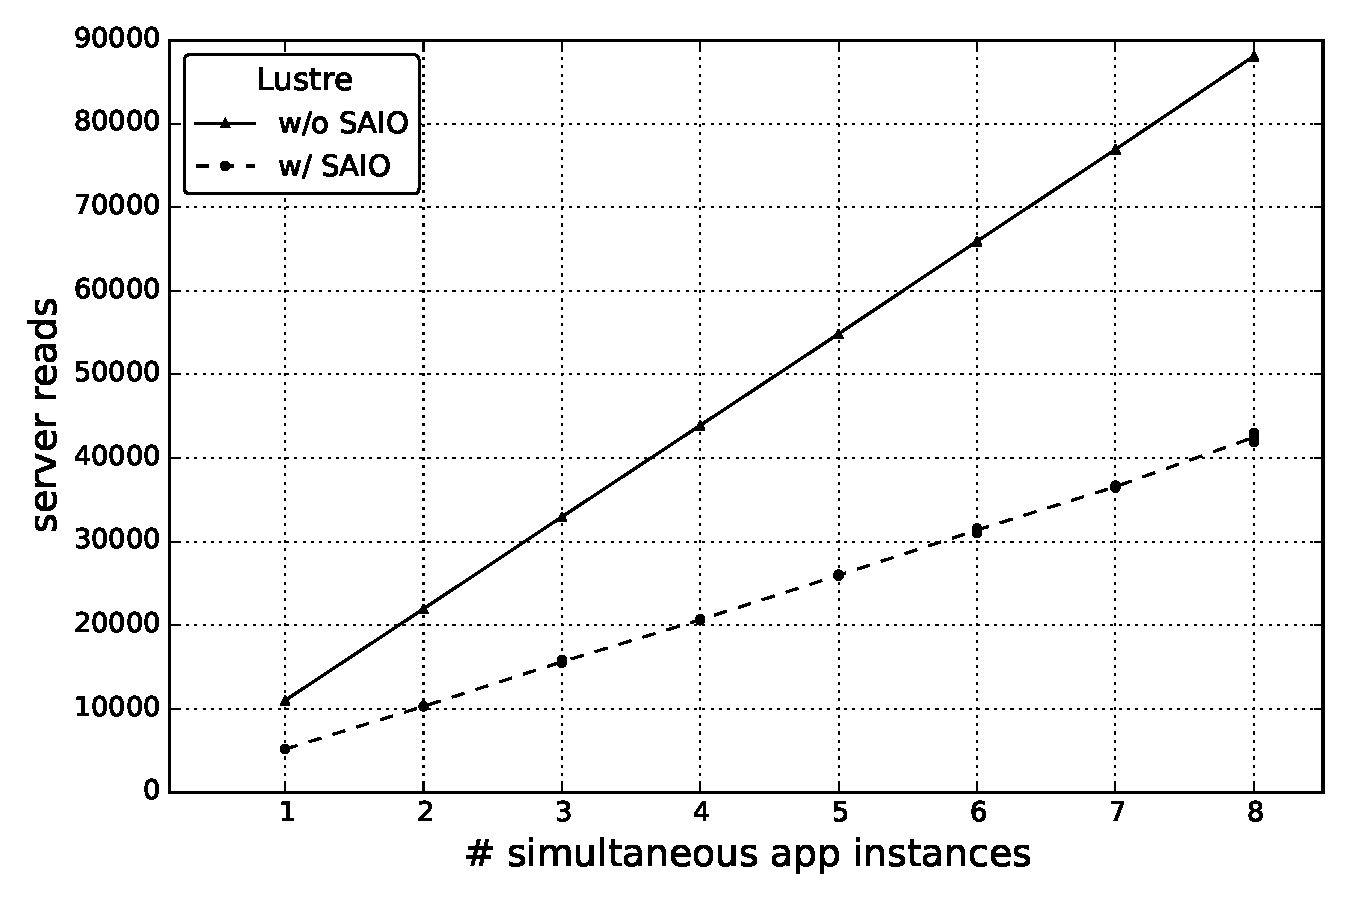
\includegraphics[width=\textwidth]{figures/reads_multiple_simult_procs_Lustre_testcluster}
    \caption{\textit{}}
    \label{figure: lustre_4}
  \end{subfigure}
  \caption{Reads processed by local ext4, GPFS and Lustre I/O servers for multiple instances of ROOT accessing a file of 5 GB (\ref{figure: ext4_4},~\ref{figure: gpfs_4} and~\ref{figure: lustre_4}).}
  \label{figure: read_2}
\end{figure*}

As far as Figures~\ref{figure: ext4_2},~\ref{figure: gpfs_2} and~\ref{figure: lustre_2} are concerned, these account for the effect of processes' concurrency on the file system. 
Before continuing with the discussion we have to make a note here. In our architecture, only one process per file system's client issues (through multiple \textit{Advisor Thread}s) 
hints on behalf of running applications. This introduces some overhead, since we have to pass the access information from the \textit{Assisted I/O library} to the \textit{Advice Manager}, 
but has the advantage of better coordinating accesses to the same file from multiple processes. Nevertheless, we found that in the case of GPFS, despite the fact of having multiple 
\textit{Advisor Thread}s, only one process among the many was receiving a benefit from the prefetching hints; the reason is that GPFS seems to have the restriction of hinting only one 
file per process. For this reason, we developed another variant of Mercury in which the AIO library, now renamed \textit{Self Assisted I/O library} (SAIO), internally provides the 
creation and the handling of multiple \textit{Advisor Thread}s. 

Looking at the figures generated with the new SAIO library we can assess the effectiveness of the prefetching hints for 
the three file systems considered. In particular, Lustre provides the best run-time improvements compared to the case in which no hints were used. GPFS shows a more contained improvement 
since the I/O time is already small compared to Lustre and ext4. Finally, ext4 can really benefit from prefetching hints especially for high process counts. Overall, excluding ext4, when 
we increase the number of processes the run-time improvements shrink. Because ext4 transfers data directly from the local SATA HDD, in which I/O time is dominated by disk latency, we can 
still improve performance as the number of application instances increases by making efficient use of the cache to hide such latency. GPFS and Lustre servers, on the other hand, have much 
higher transfer performance compared to single disk ext4 and both use a network link to move data across the network; GPFS uses the NSD protocol while Lustre uses the LNET protocol. For GPFS
and Lustre network bandwidth becomes critical and, in fact, as the number of instances increases the run-time decreases because of the saturation of the network link in the node.

Figure~\ref{figure: ext4_3},~\ref{figure: gpfs_3} and~\ref{figure: lustre_3} report the number of read requests accounted for by the different file systems under study. More specifically, 
the figures show how the number of reads at the I/O server side for both GPFS and Lustre can be substantially reduced with our approach. This has a significant impact in HPC cluster in 
which the file system may be accessed by many thousand of processes at the same time. Reducing the number of requests for an application can increase the number of IOPS available for others. 
This result is also confirmed for multiple instances of the `ROOT' application running concurrently (Figure~\ref{figure: ext4_4},~\ref{figure: gpfs_4} and~\ref{figure: lustre_4}).

\subsection{Conclusions}
Our experiments have focused on prefetching performance in a real scenario setup. In particular we have considered the cache utilization by a single application's instance as well as the
combined cache utilization by multiple application's instances. We have shown how in both cases we can reduce the application runtime by aggressively prefetching data into main memory using
our transparent approach. However, since our strategy is bandwidth bound we have seen that in the case of multiple application's instances such approach leads to the saturation of the
network link in the case of networked file systems and ultimately to the shrinking of the performance gain.

%One important aspect to consider in HPC is that although nodes typically run only a single application at a time, there might
%be still multiple instances of it operating on different parts of the input dataset (SPMD model). As we have mentioned in Chapter~\ref{chapt: introduction} the number of cores in HPC nodes
%is increasing faster than the amount of available memory per core. This, combined with the fact that prefetching performance are limited by the saturation of the network link in the case of
%intense I/O activity, poses a further criticality on optimal cache management policies. In this sense, our solution provides effective control over the cache utilization to the user, that can
%thus make sure that unneeded pages are explicitly evicted from the cache using hints, saving up space for more valuable pages and reducing the network traffic from the network file system.

\section{Write Behind in Collective I/O}
To evaluate the proposed MPI-IO hints we use three popular I/O benchmarks frequently adopted to profile collective I/O performance in other research works: 
coll\_perf\footnote{Collective I/O benchmark distributed with the MPICH package.}, Flash-IO and IOR. The main difference between these three benchmarks is 
the amount of data written per I/O and access pattern. In fact, coll\_perf writes all the strided data (32~GB) in a single collective I/O operation using 
\texttt{MPI\_File\_write\_all()}, Flash-IO writes small amounts of strided data (in the order of few MB) over multiple collective I/O operations using 
\texttt{MPI\_File\_write\_at\_all()}, and finally IOR writes larger amounts of contiguous data than Flash-IO (4~GB) over multiple collective I/O operations.

Minor changes to the source code of the three benchmarks have been made to adapt them to our needs. For example, coll\_perf and Flash-IO did not support writing 
to multiple files or the emulation of computing time between writes. Thus, we modified them to reproduce a workflow similar to the one shown in Figure~\ref{figure: workflow}. 
The number of written files and a compute time are now parameters that can be passed from the command line. In all our tests we used 512 MPI processes distributed over 
64 nodes (8 procs/node), fixed the file stripe size to 4~MB and the stripe count to 4. Moreover, for simplicity, we also fixed the size of the cache synchronisation 
buffer (i.e. \codeword{ind\_wr\_buffer\_size}) to 512~KB, which corresponds to the standard independent I/O buffer size. On the other hand, we varied the collective 
I/O parameters, i.e., the number of aggregators (from 8 to 64) and the collective buffer size (from 4~MB to 64~MB). 
For every combination of the described parameters (<aggregators>\_<coll\_bufsize>) each benchmark writes four files of the same size (32~GB) with a compute delay of 30 seconds, 
which is in most cases enough to hide the synchronisation time. We compute the bandwidth as the average bandwidth over the four collective write operations (Equation~\ref{formula: abw}). 

The different contributions within the collective I/O write path shown in Figure~\ref{figure: coll_io_impl} are extracted from the ROMIO layer using MPE profiling
~\cite{Gropp2014}. Whenever the compute delay is not enough to hide synchronisation cost (e.g. when a small number of aggregators is used), the remaining synchronisation 
time is added to the total write time, thus reducing the bandwidth.

\subsection{Testbed}
Our testbed is a research cluster designed and developed in the context of the DEEP/-ER~\cite{Eicker2013} projects (Dynamic Exascale Entry Platform/-Extended Reach). The 
DEEP/-ER cluster has 2048 cores distributed over 128 computing nodes (dual socket Sandy Bridge architecture). The storage system is composed of 6 Dell PowerEdge 
R520 servers equipped with 2 Intel Xeon Quad-core CPUs and 32~GB of memory and run the BeeGFS file system from Fraunhofer ITWM~\cite{Heichler2014}
(formerly known as FhGFS). The servers are connected to a SGI JBOD with 45 2TB SAS drives through a SAS switch using two 4x ports at 6~GB/s, for a total of four 
8+2 RAID6 storage targets and 2 RAID1 targets for metadata and management data (1 drive is left as spare). One of the six I/O servers is dedicated as metadata 
server, one as management server and the remaining four as data I/O servers.
Additionally, every compute node is equipped with 32~GB of RAM memory and a 80~GB SATA SSD containing the operating system plus an additional 30~GB ext4 partition 
(mounted under `/scratch') for general purpose storage. This partition, in our case, is used to locally cache collective writes. Finally, all the computing nodes 
are connected through an Infiniband QDR network and use ParaStation MPI\footnote{\url{http://www.par-tec.com/products/parastation-mpi.html}.} (PSMPI) version 5.1.0-1 
as message passing library.

\subsection{Performance Results}
We measured collective I/O performance using Formula~\ref{formula: bw} and~\ref{formula: abw} for the application perceived bandwidth. Additionally, we also measured
the effect of the single ext2ph contributions to collective I/O, as reported in Figure~\ref{figure: coll_io_impl}. In the rest of this section we present our findings
for the three target benchmarks.

\subsubsection{Coll\_perf}
Coll\_perf is a synthetic benchmark that performs collective I/O to a shared file using a single collective write operation. The application uses a three-dimensional
dataset partitioned and assigned to available processes using a block-block strategy~\cite{Bordawekar1993}, that is, the original input domain is divided into a number of blocks equal to the 
number of processes, and each is assigned to a process. Each block is afterwards written to the file using a row-major order. In our configuration we use 512 processes 
distributed over 64 nodes of the 128 available in the DEEP cluster. Every process handles a block with $256 \times 256 \times 256$ integer elements, for a total 64~MB of data
per process and 32~GB for the whole file.

In our experiments we measured three values of write bandwidth: 

\begin{itemize}
\item the bandwidth when the cache is disabled (this is the default case) and collective I/O writes data to the global file system directly (\textit{BW Cache Disable}); 
\item the bandwidth when the cache is enabled and data is flushed immediately to the global file system (\textit{BW Cache Enable}); and 
\item the bandwidth when the cache is enabled but data is not flushed to the global file system (\textit{TBW Cache Enable}). 
\end{itemize}

The latter gives us a theoretical bandwidth figure (TBW) that we can use to estimate how well the cached collective I/O implementation is doing. In order to measure the potential 
benefits of our cached approach we modify the workflow in Figure~\ref{figure: workflow} moving the write phase before the compute phase. In this way we can always overlap cache 
synchronization with compute.

\begin{figure*}[]
  \centering
  \begin{subfigure}[]{0.7\textwidth}
  \centering
  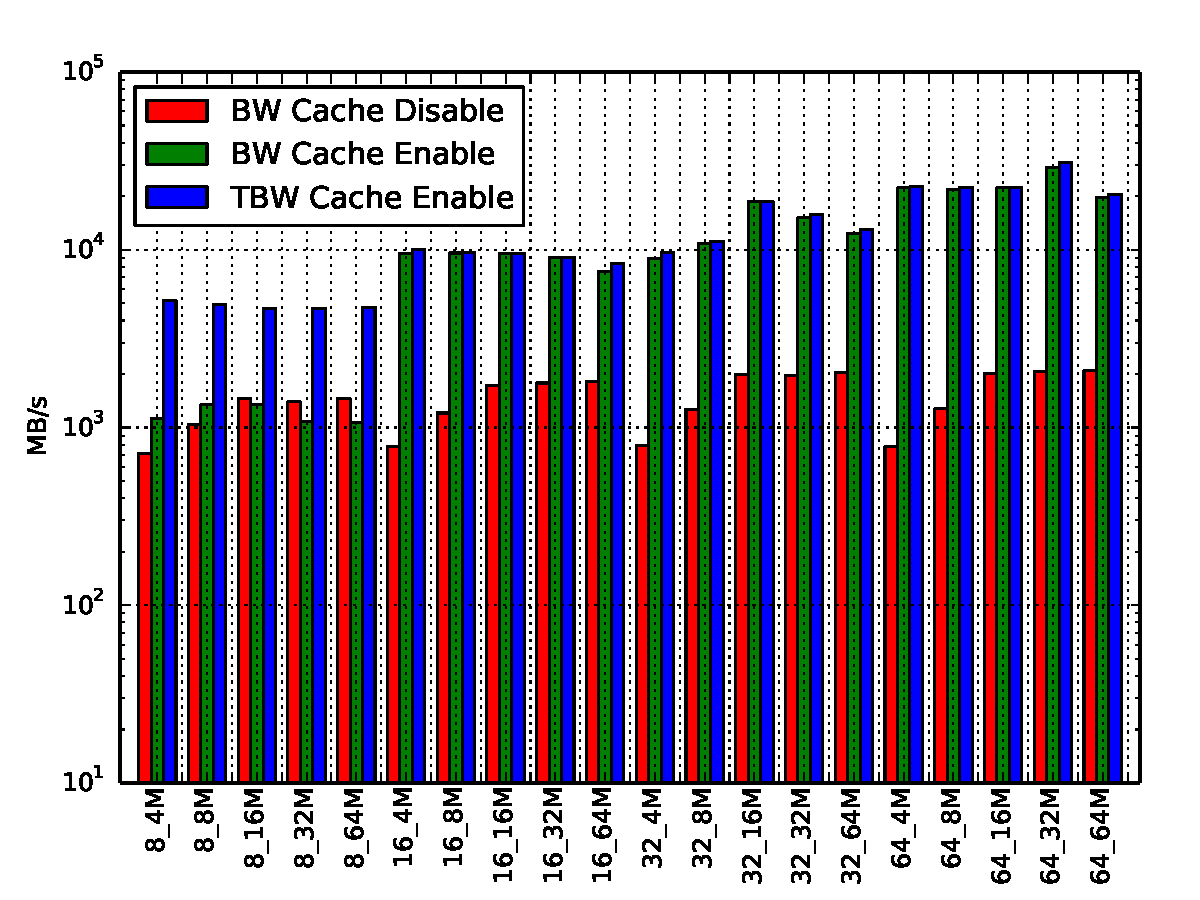
\includegraphics[width=\textwidth]{figures/coll_perf_32GB_30sec_bw}
  \caption{}
  \label{figure: collperf-bw}
  \end{subfigure}
  \begin{subfigure}[]{0.7\textwidth}
  \centering
  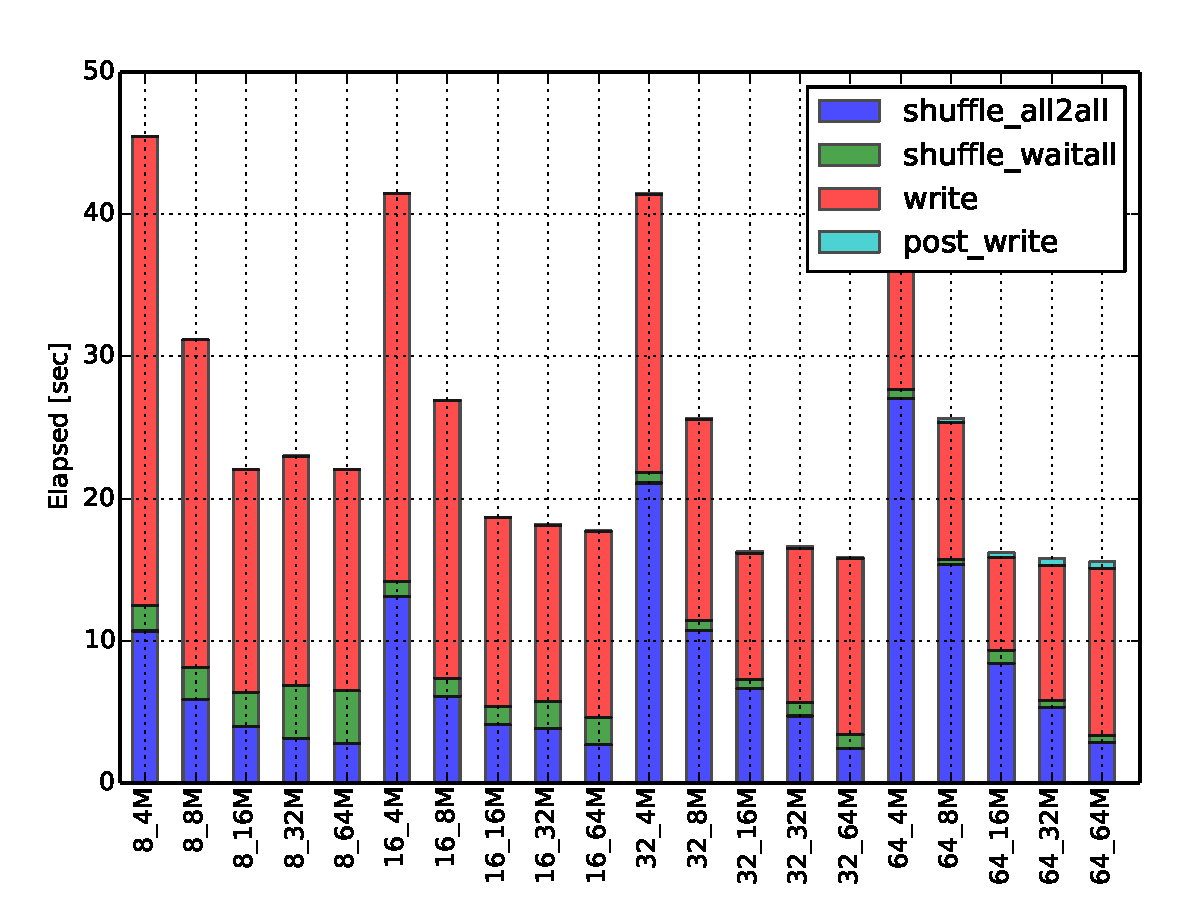
\includegraphics[width=\textwidth]{figures/coll_perf_32GB_30sec_elapsed_disable}
  \caption{}
  \label{figure: collperf-elaps-disable}
  \end{subfigure}
  \begin{subfigure}[]{\textwidth}
  \centering
  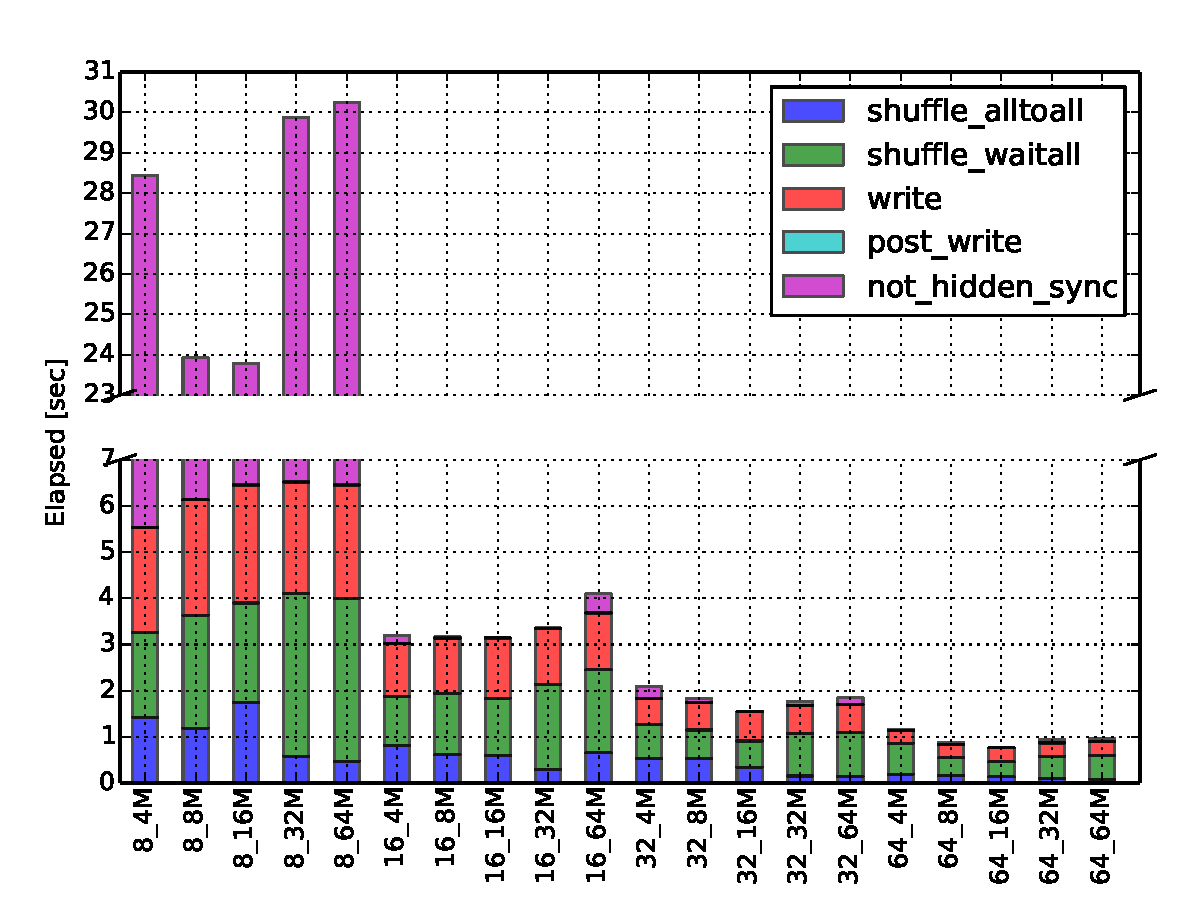
\includegraphics[width=0.7\textwidth]{figures/coll_perf_32GB_30sec_elapsed_enable}
  \caption{}
  \label{figure: collperf-elaps-enable}
  \end{subfigure}
  \caption{Perceived and theoretical write bandwidth for all combinations of aggregators and collective buffer sizes (\ref{figure: collperf-bw}); 
  collective I/O contribution breakdown when cache is disabled (\ref{figure: collperf-elaps-disable}); collective I/O contribution breakdown when cache is 
  enabled (\ref{figure: collperf-elaps-enable}).}
  \label{figure: collperf-results}
\end{figure*}

Figure~\ref{figure: collperf-results} shows the results for the perceived and theoretical write bandwidth (\ref{figure: collperf-bw}), as well as the single 
performance contributions for standard collective I/O (\ref{figure: collperf-elaps-disable}) and cached collective I/O (\ref{figure: collperf-elaps-enable}). 
We start by analyzing the behaviour of standard collective I/O in Figure~\ref{figure: collperf-elaps-disable}.

Let us start by considering the effect of different collective buffer sizes on the collective write time. To this purpose we fix the number of aggregators and look at 
the time contributions when increasing the buffer size from 4~MB to 64~MB. We first observe that the global synchronization cost (\textit{shuffle\_all2all}) decreases.
This is consistent with the ext2ph algorithm behaviour because, as we have already said, increasing the collective buffer size decreases the number of two phase I/O rounds
and therefore the number of global synchronization events (\texttt{MPI\_Alltoall()}). The write cost associated to POSIX write operations also decreases because we are
writing to more I/O servers at the same time (recall that we are using four I/O servers and a stripe size of 4~MB). When the buffer size is 4~MB we only write to one
I/O server, when the buffer size is 16~MB we write to all of them. This also explains why further increasing the buffer size does not reduce the write cost. The
communication cost (\textit{shuffle\_waitall}), on the other hand, increases with the buffer size. This happens because, although the total amount of data shuffled remains
constant, the amount of data shuffled during every round of two phase I/O increases, saturating the aggregators network bandwidth. When we use 8 aggregators, for example, 
up to 32~MB of data are shuffled across the network when using 4~MB buffers, up to 512~MB with 64~MB buffers. Finally, we can look at what happens when we keep the
buffer size constant and increase the number of aggregators. In this case we notice that the global synchronization cost increases. This is due to the increased network 
concurrency at the I/O servers. Finally, \textit{post\_write} time, represented by \texttt{MPI\_Allreduce()}, does not contribute considerably to overall performance because
the corresponding global synchronization event is only encountered once.

We now look at what happens to the ext2ph contributions when we use the cache (Figure~\ref{figure: collperf-elaps-enable}). The global synchronization cost can be still reduced
by increasing the collective buffer size, but because local SSDs are not shared with other nodes across the network, I/O requests can be served in a more predictable way. This
allows aggregators to complete I/O faster and consequently reduces the global synchronization overhead related to collective communications. Write time is not affected visibly
by larger buffers because every aggregator writes data locally. Communication cost is not affected because the communication pattern does not change with respect to the non-cached
collective I/O case. Additionally, we now have a new contribution representing the cache synchronization time that cannot be overlapped with computation (\textit{not\_hidden\_sync}).
We can observe that this contribution is consistent only for 8 aggregators. In fact, when using 8 aggregators the aggregated bandwidth provided by the local SSD
devices cannot match the parallel file system.

The described behaviours are reflected on the perceived write bandwidth shown in Figure~\ref{figure: collperf-bw}. In particular we observe that only the 8 aggregators
configuration achieves worse performance than the standard collective I/O case. All the remaining configurations always achieve better performance and can provide up to
30~GB/s when using 64 aggregators and 32~MB buffer size, an improvement of 15 times. We also observe that the aggregated bandwidth can be scaled by increasing the number 
of aggregators and thus the number of available SSD devices. Finally, when using the cache, the buffer size has limited impact on write bandwidth meaning that we can achieve 
good performance with small buffer sizes, reducing the pressure of collective I/O on system memory.

\subsubsection{Flash-IO}
Flash-IO is the I/O kernel of the Flash application~\cite{Rosner2000}. The Flash-IO benchmark writes three different
files, a checkpoint file a plot file with centered data and a plot file with corner data. The checkpoint file is written using either parallel HDF5 or PnetCDF. We modified the
benchmark to only write the checkpoint file using parallel HDF5. In our configuration, every process in the Flash application writes 80 blocks. Each block contains 16 zones, and 
each zone has 24 variables encoded with 8~bytes, for a total of 768~KBs/block/proc, for a total file size of about 30~GB. Blocks are not written to the checkpoint file with a 
single collective write operation, like in coll\_perf, but instead using multiple collective operations through \texttt{MPI\_File\_write\_at\_all()}. Similarly to coll\_perf we 
have modified the Flash-IO workflow to completely hide the cache synchronization cost.

\begin{figure*}[]
  \centering
  \begin{subfigure}[]{0.7\textwidth}
  \centering
  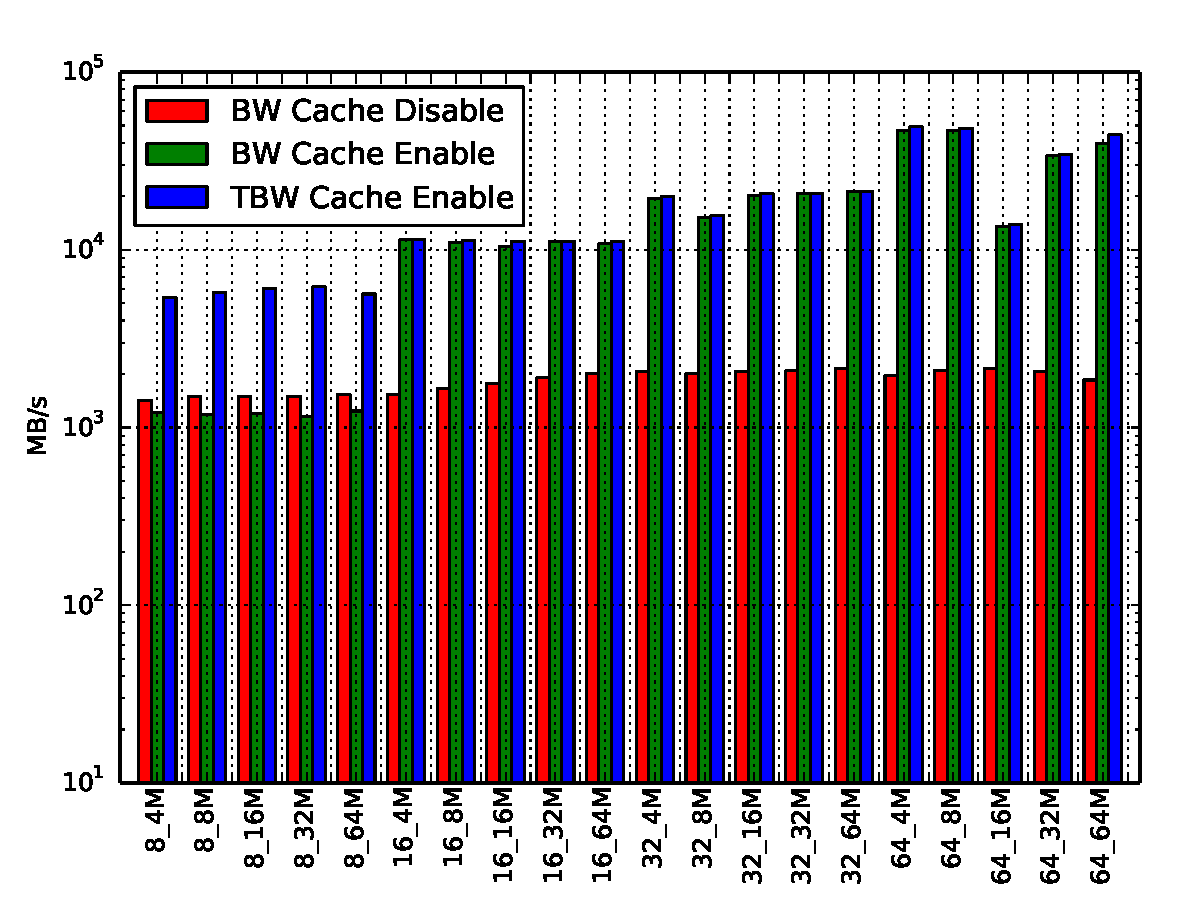
\includegraphics[width=\textwidth]{figures/flash_32GB_30sec_bw}
  \caption{}
  \label{figure: flash-bw}
  \end{subfigure}
  \begin{subfigure}[]{0.7\textwidth}
  \centering
  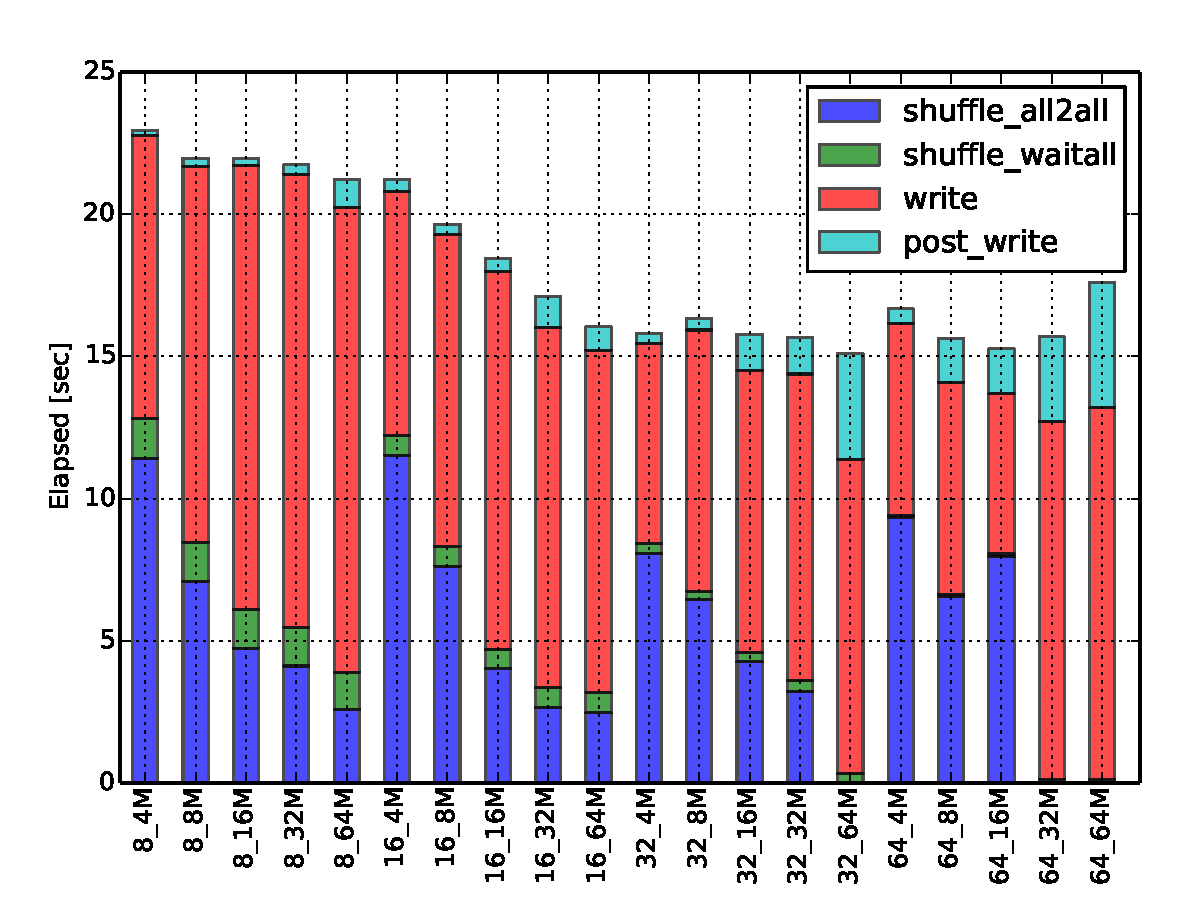
\includegraphics[width=\textwidth]{figures/flash_32GB_30sec_elapsed_disable}
  \caption{}
  \label{figure: flash-elaps-disable}
  \end{subfigure}
  \begin{subfigure}[]{\textwidth}
  \centering
  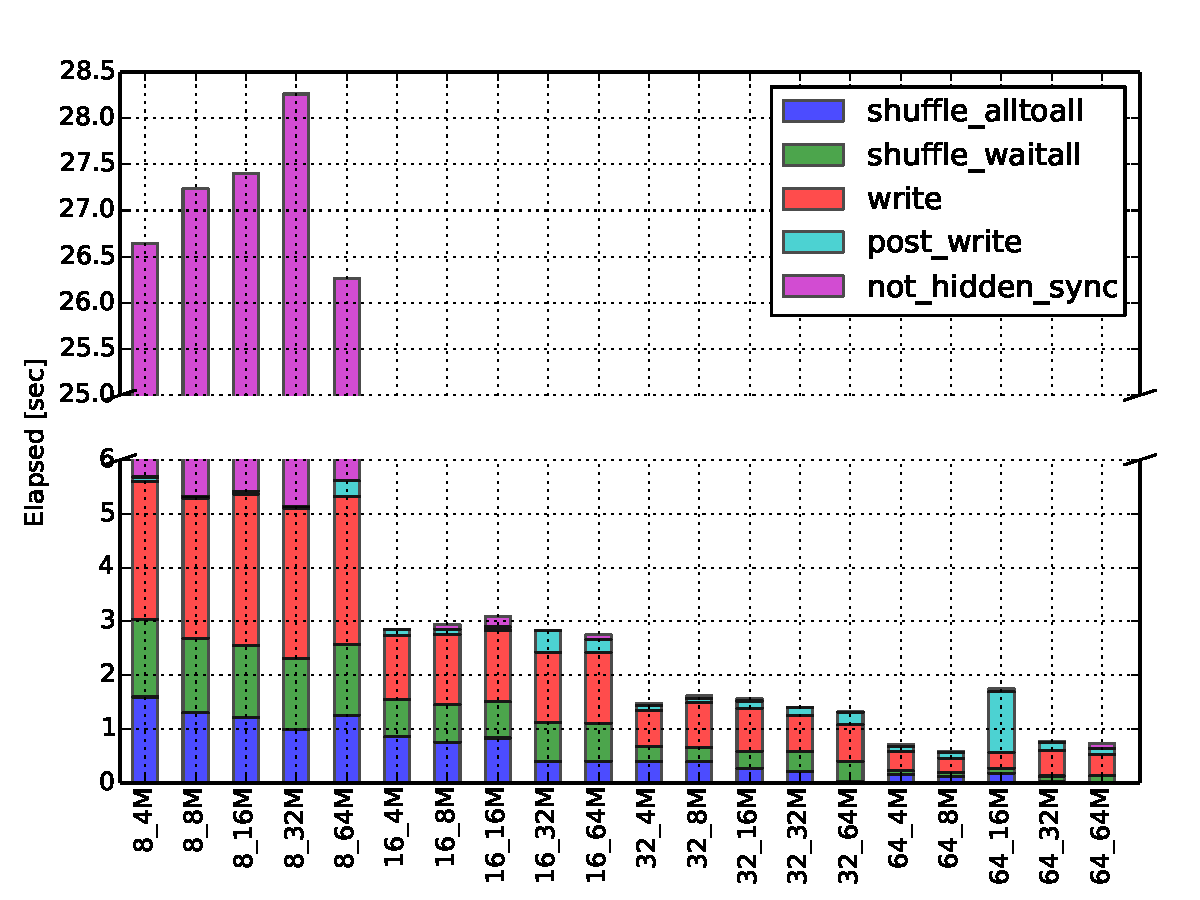
\includegraphics[width=0.7\textwidth]{figures/flash_32GB_30sec_elapsed_enable}
  \caption{}
  \label{figure: flash-elaps-enable}
  \end{subfigure}
  \caption{Perceived I/O bandwidth for all combinations of aggregators and collective buffer sizes (\ref{figure: flash-bw}); collective I/O contribution breakdown 
  when cache is disabled (\ref{figure: flash-elaps-disable}); collective I/O contribution breakdown when cache is enabled (\ref{figure: flash-elaps-enable}).}
  \label{figure: flash-results}
\end{figure*}

Like in coll\_perf, for Flash-IO we measured the same performance parameters varying the number of aggregators and collective buffer size. Results are shown in Figure~\ref{figure:
flash-results}. When the cache is disabled, again we observe reduction of the global synchronization cost for increasing buffer sizes. Communication cost this time does not increase 
with the buffer size. In fact, the file domain size varies from about 49~MB to 6~MB, for 8 and 64 aggregators respectively. This is much less than the amount of data exchanged in 
coll\_perf and thus can be better served by the network infrastructure. Write performance, on the other hand, get worse as the buffer size increases. This behaviour is probably due 
to the fact that, unlike in coll\_perf, writes are not multiple of the stripe size and therefore there might be additional locking overhead at the file system level.
Finally, we observe that the \textit{post\_write} contribution is more consistent this time. The reason, as already anticipated, is that Flash-IO does not write data with a single
collective operation but instead uses multiple operations, thus increasing the number of \texttt{MPI\_Allreduce()} calls at the end of the ext2ph algorithm.

When the cache is enabled we can observe much better performance. Once again, 8 aggregators are not sufficient to completely hide cache synchronization cost to the application. As last
note, we see that in the case of 64 aggregators and 16~MB buffer size there is a drop of write bandwidth in Figure~\ref{figure: flash-bw} due to a peak in the \textit{post\_write}
contribution in Figure~\ref{figure: flash-elaps-enable}. This tells us that when using the cache, although we can minimize the scheduling effects on I/O requests, a small variation 
in the I/O time across aggregators can produce substantial effects on the perceived bandwidth. Indeed, we can see a drop of about 25~GB/s with respect to the 64 aggregators and 
32~MB buffer size.

\begin{figure*}[]
  \centering
  \begin{subfigure}[]{0.7\textwidth}
  \centering
  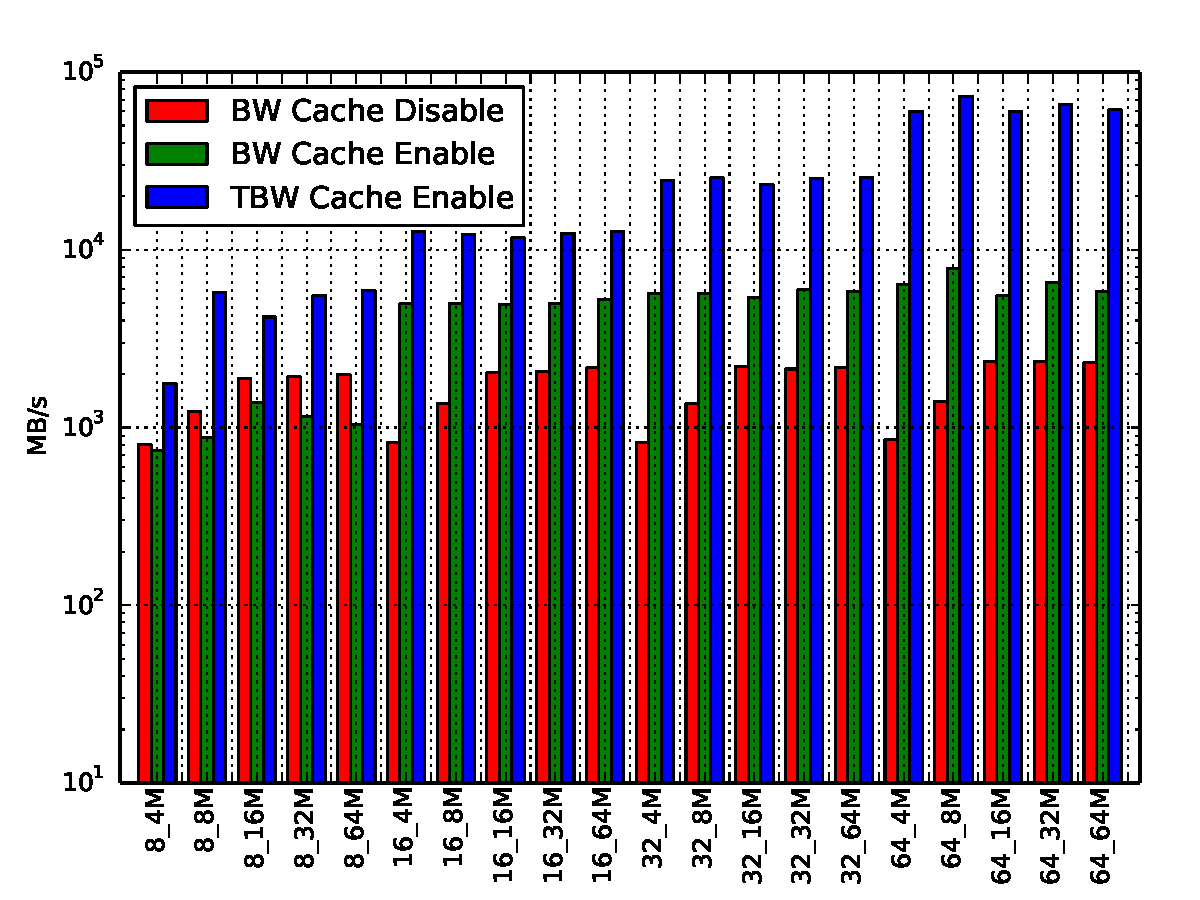
\includegraphics[width=\textwidth]{figures/ior_32GB_30sec_bw}
  \caption{}
  \label{figure: ior-bw}
  \end{subfigure}
  \begin{subfigure}[]{0.7\textwidth}
  \centering
  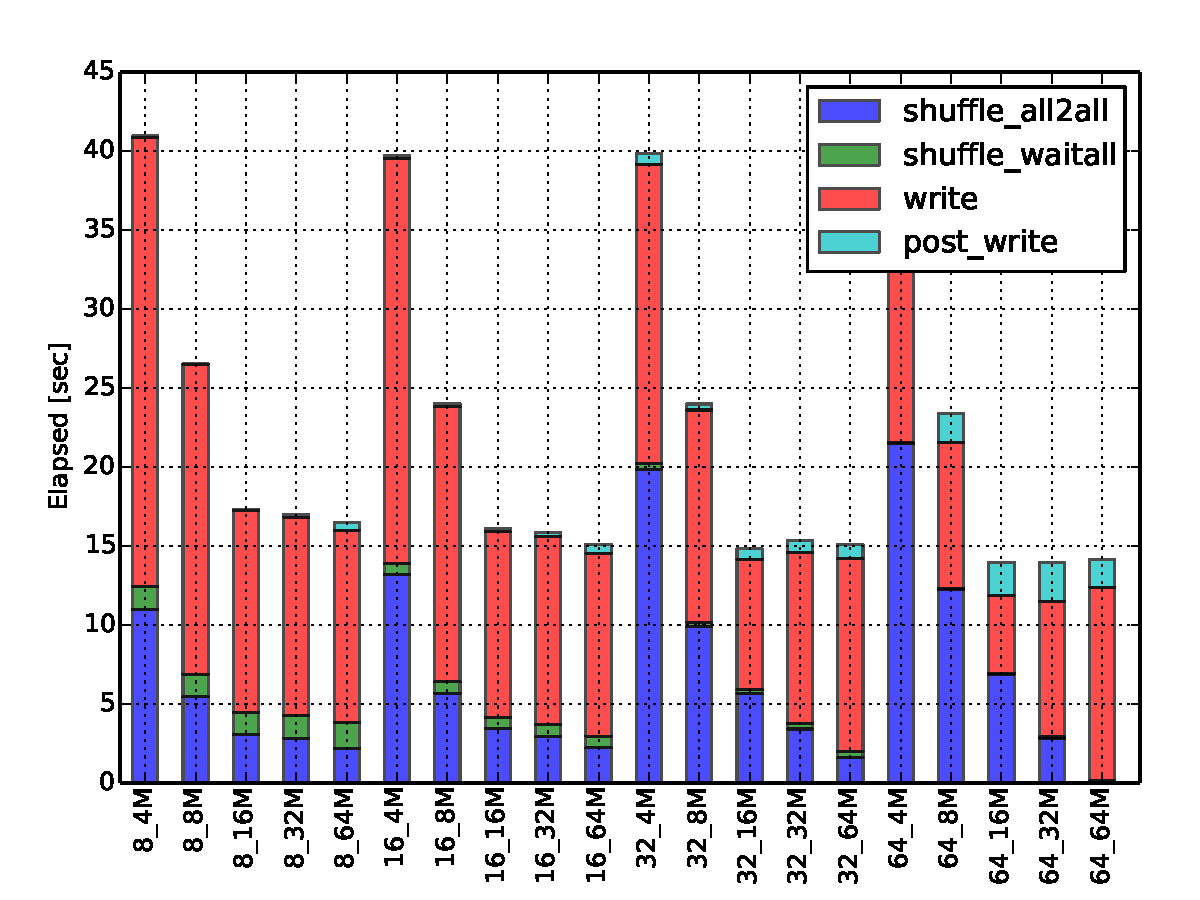
\includegraphics[width=\textwidth]{figures/ior_32GB_30sec_disable}
  \caption{}
  \label{figure: ior-elaps-disable}
  \end{subfigure}
  \begin{subfigure}[]{\textwidth}
  \centering
  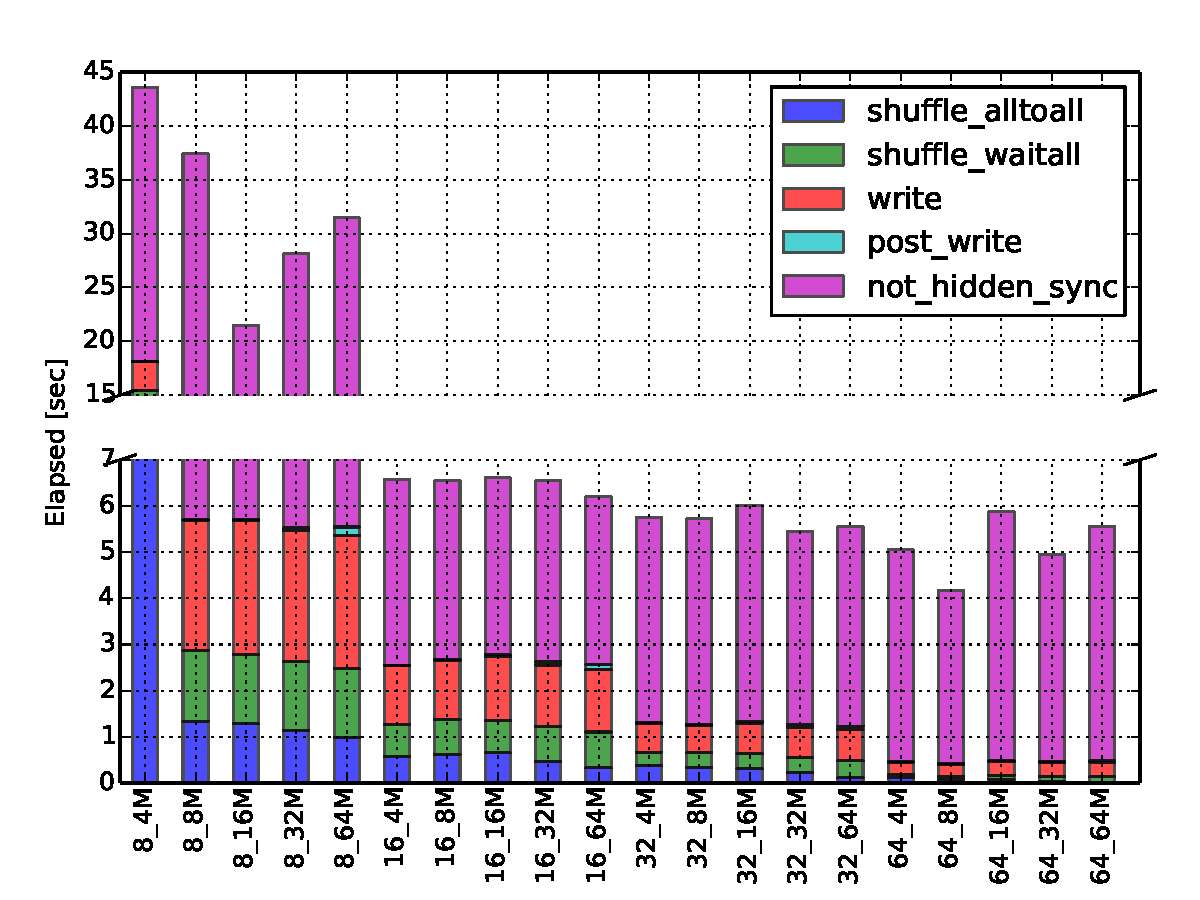
\includegraphics[width=0.7\textwidth]{figures/ior_32GB_30sec_enable}
  \caption{}
  \label{figure: ior-elaps-enable}
  \end{subfigure}
  \caption{Perceived I/O bandwidth for all combinations of aggregators and collective buffer sizes (\ref{figure: ior-bw}); collective I/O contribution breakdown when cache is 
  disabled (\ref{figure: ior-elaps-disable}); collective I/O contribution breakdown when cache is enabled (\ref{figure: ior-elaps-enable}).}
  \label{figure: ior-results}
\end{figure*}

\subsubsection{IOR}
IOR\footnote{\url{http://www.nersc.gov/users/computational-systems/cori/nersc-8-procurement/trinity-nersc-8-rfp/nersc-8-trinity-benchmarks/ior/}.} is a parallel I/O benchmark that supports 
both independent and collective I/O operations using a variety of interfaces including POSIX-IO, MPI-IO and HDF5. Although IOR supports collective I/O operations it does not allow
users to define strided patterns (like the one in coll\_perf) using file views. Strided layouts can be built by reading or writing multiple data segments. A segment is a contiguous byte 
range in the file accessed by only one process. For example, if we have four processes and each of them writes three segments of 64~MB, the first process writes its first segment
starting at 0~MB and ending at 64~MB, the second process writes its first segment starting at 64~MB and ending at 128~MB, and so on.
When all the processes have written the first segment they initiate another write operation for the second segment starting at offset 256~MB. Every segment is written with an independent
collective write operation.

In our experiments we used 8 segments and each of the 512 processes writes 8~MB for segment, for a total of 32~GB file. Unlike the previous two cases, in IOR we follow the workflow
depicted in Figure~\ref{figure: workflow}; meaning that for the last write phase cache synchronization will not be hidden by any following compute phase. This allows us to show what 
a real world use case would look like.

Figure~\ref{figure: ior-results} shows the obtained results. These results are similar to the previous except for the fact that now the \textit{not\_hidden\_sync} contribution is
visible for every collective I/O configuration. The cache synchronization cost represents a huge part of the total I/O time. Although, absolute bandwidth performance are lower 
than previous results we still have that writing data to local SSD devices can give advantages over the baseline ext2ph strategy. In fact, on average we can at least triple the 
perceived write bandwidth going from about 2~GB/s to 6~GB/s.

The reduction of the cache synchronization cost has not been explored in our work and therefore leaves opening for future optimizations that will be discussed in the conclusion
chapter.

\subsection{Conclusions}
In this section we have analyzed collective write performance using a range of different benchmarks that use both synthetic and real I/O patterns to transfer large checkpoint buffers
to the parallel file system. Our tests show how collective I/O is mainly limited by the ext2ph algorithm global synchronization overhead and how the use of fast local non-volatile
memories is effective in reducing the impact that global file system latency has on such synchronization by taking it out of the critical I/O path. Our work practically proves
how next generation I/O systems can benefits from multi tier storage and how first tier non-volatile storage devices can be leveraged by giving the user more control over them.

%!TEX root = ../main.tex
\section{Related Work}
\label{sec: related}

Many research works have tried to optimise collective I/O focusing on different aspects. Yu and Vetter~\cite{WeikuanV08} before us have identified the global synchronisation problem as one of the most severe for collective I/O performance. They exploited access pattern characteristics, common in certain scientific workloads, to partition collective I/O into smaller communication groups and synchronise only within these. Block-tridiagonal patterns, not directly exploitable, are automatically reduced, through an intermediate file view, to a more manageable pattern and can thus take advantage of the proposed solution. The ADIOS library~\cite{CPE:CPE3125} addresses this problem similarly by dividing a single big file into multiple files to which collective I/O is carried out independently for separated smaller groups of processes. Lu, Chen, Thakur and Zhuang~\cite{YinYTY12} further explored collective I/O performance beyond global synchronisation and considered memory pressure of collective I/O buffers. They proposed a memory conscious implementation that accounts for reduced memory per core in future large scale systems. Liao~\cite{Liao11} focused on the file domain partitioning impact on parallel file systems' performance. He demonstrated that by choosing the right file domain partitioning strategy, matching the file system locking protocol, collective write performance can be greatly improved. Yong, Xian-He, Thakur, Roth and Gropp~\cite{YongXTRG11} addressed the problem of I/O server contention using a layout aware strategy to reorganize data in aggregators. On the same lines, Xuechen, Jiang and Davis~\cite{XuechenJD09} proposed a strategy to make collective I/O `resonant' by matching memory layout and physical placement of data in I/O servers and exploiting non-contiguous access primitives of PVFS2. The strategy proposed is similar in concept to the Lustre implementation of collective I/O in which file contiguous patterns are converted to stripe contiguous patterns and the concurrency level on OSTs can be set using the MPI-IO hint \codeword{romio\_lustre\_co\_ratio} (Client-OST ratio). Liu, Chen and Zhuang~\cite{JilianYY13} exploited the scheduling capabilities of PVFS2 I/O servers to rearrange I/O requests' order and better overlap read and shuffle phases among different processes. 

Lee, Ross, Thakur, Xiaosong and Winslett~\cite{LeeRTXW04} proposed RTS as infrastructure for remote file access and staging using MPI-IO. Similarly to our approach, RTS uses additional threads, Active Buffering Threads (ABT)~\cite{XiaosongWLS03}, to transfer data in background to the compute phase. Moreover, the authors also modified the ABT ROMIO driver implementation to stage data in the local file system whenever the amount of main memory runs low. Although they include collective I/O in their study, they lack a detailed evaluation of the impact that SSD caching can have on the different performance contributions of collective I/O and the additional reduction of memory pressure. Furthermore, remote staging of data requires additional nodes while we collocate storage with compute. The SCR library~\cite{SCR} also uses local storage resources to efficiently write checkpoint/restart data but this is targeted to a specific use case and requires the modification of the application's source code to be integrated. Other works, focus on I/O jitter reduction using multi-threading and local buffering resources~\cite{DorierACSO12}, but we do an evaluation of collective I/O and show how the effect of I/O jitter can become even more prominent when using fast NVM devices. More recently the Fast Forward I/O project~\cite{fastforward}, from U.S. Department of Energy (DOE), proposed a burst buffer architecture to absorb I/O bursts from file system clients into a small number of high performance storage proxies equipped with high-end solid state drives. This technique has been, e.g., implemented in the DDN Infinite Memory Engine~\cite{DDN}. Even though the burst buffer solution is interesting, it may require very expensive dedicated servers as well as significant changes to the storage system architecture. 

Unlike previous works, we proposed a fully integrated, prototype solution for new available memory technologies able to scale aggregate bandwidth in collective I/O with the number of available compute nodes. Additionally, our solution does not require any proprietary hardware or dedicated kit to work. We demonstrate that SSD based cache can reduce the synchronisation overhead intrinsic in the collective I/O implementation in ROMIO as well as the requirement for large collective buffers (memory pressure). Our implementation is compatible with legacy codes, since it does not require any change at the application level, and can work out of the box with any backend file system, although in DEEP-ER we focused on BeeGFS. At the moment the cache synchronisation is implemented in the ADIO UFS driver using pthreads. Future releases of BeeGFS will support native caching, including asynchronous flushing of local files to global file system. We have already integrated ROMIO with a BeeGFS driver that will take advantage of these functionalities.

%!TEX root = ../main.tex
\section{Conclusion \& Future Work}
\label{sec: mercury_conclusion}

In this chapter we presented a guided I/O framework prototype that can be used to set POSIX advice and GPFS hints on behalf of applications transparently to the user. This is done by adding annotations regarding which regions of a file to prefetch into a configuration file that is afterwards fed to the \textit{Assisted I/O library} and \textit{Advice Manager} modules. %We demonstrated that using our prototype the non-optimal I/O pattern of a real application can be adapted to the underlying storage system to improve performance. %This is useful for all those applications that access their data using an immutable I/O pattern, like the `ROOT' application here presented.

%We focused predominantly on read patterns which characterize a class of scientific applications known as big data science analytics. These class of applications differ from HPC applications in the type of I/O pattern they use. Indeed, HPC applications are dominated by writing of large amounts of checkpoint data to a shared (N-1 pattern) or multiple files (N-N pattern) for restart purposes or, more generally, for post processing. Big data analytics applications, on the other hand, read large amounts of input data for processing and write very little volumes of output data (results) to the file system. Currently, there is a convergence of these two paradigms that brings big data analytics applications to run on high-end computing clusters, typically as post processing phase for data generated by HPC applications such as, e.g., climate and earthquake simulations. Here we considered `ROOT' as representative for big data science analytics and we demonstrated that by using the hints API provided by the file system in an appropriate way it is possible to improve the storage system usage and ultimately the application performance.  
 
In the future we plan to further explore the problem of data science analytics applications in HPC, studying more profusely the different types of existing I/O patterns and how hints can be used to improve the cache utilization efficiency and thus applications' performance. Moreover, although not explicitly treated here, we recognise how important is to automatically extract information concerning the application's I/O pattern profile. Almost all the current analysis tools, including the ones we have used, approach the I/O pattern analysis problem from an ultra fine-grain point of view (i.e. considering the offset and length requests) with the result of having a very specific file per application characterization. On the other hand, in this work we have observed that a course-grain approach (i.e. considering blocks instead of single requests) can be more beneficial when trying to extract the general application behaviour. The study of an automatic I/O pattern analysis tool with the described features will be thus part of future work. 
%In the future we plan to extend the \textit{Advice Manager} to provide support for MPI I/O hints that currently have to be hard coded into the application. In this way administrators could use our mechanism to change, for instance, the striping policy of a specific file to adapt it to the underlying storage system configuration, without modifying the application. The integration of cluster aware I/O support will also compensate for the lack of file access global scope in the current version. 

%TODO: consider a comment about how this won't work as a cluster-aware installation - open files are not shared between nodes, they have an independent view. 

%TODO: a criticism may be that 'we never run the application with the same data', and 'changing the data changes the applications behaviour', so the learning approach isn't valid. A sentence or two to explain that while the data may change, the manner in which the program accesses it does not. A good example of this is a climate simulator.


\section*{Acknowledgment}
This work has been funded by the FP7 program of the European Commission through the DEEP-ER project (Grant Agreement no. 610476) and supported by the Exascale1O (E10) initiative.

\bibliographystyle{IEEEtran}
\bibliography{bibliography}

\end{document}
